\documentclass[a4paper,14pt]{extreport}
%Римская богиня Фортуна в эпоху Республики и начала Империи.
%The Roman goddess Fortuna in the period of the Republic and the Early Empire.
\usepackage[14pt]{extsizes} % Задаём размер шрифта 14 пунктов
\usepackage{pscyr} % Подключаем хорошие русские шрифты
\renewcommand{\rmdefault}{ftm} % Устанавливаем шрифт по умолчанию Times New Roman
% Подключаем поддержку языков. NB! русский должен идти последним - это будет язык по умолчанию.
\usepackage[greek,latin,english,french,german,italian,russian]{babel}
\usepackage[T2A]{fontenc}
\usepackage[utf8]{inputenc}
\usepackage{cmap}

% Подключаем поддержку диакритики для древнегреческого шрифта
\languageattribute{greek}{polutoniko}

% Греческие шрифты
% grmn is an excellent greek font!
% gsmi, gsmo - тоже несколько неплохо, без засечек, похожий на шрифт для печатной машинки
\newfont{\thegreek}{grmo1400} 	% Это шрифт для основного текста
\newfont{\thegreekfn}{grmo1000}	% Это шрифт для сносок
\newcommand\graeca[1]{\foreignlanguage{greek}{\thegreek{#1}}}			% Это команда греческого языка для основного текста
\newcommand\graecafn[1]{\foreignlanguage{greek}{\thegreekfn{#1}}}		% Это команда греческого языка для сносок


\renewcommand{\baselinestretch}{1.5} % Полуторный интерлиньяж
\frenchspacing
\righthyphenmin=2 % Минимальное число символов при переносе - 2.
\usepackage{indentfirst} % Включить отступ у первого абзаца
\parindent=1.27cm % Задаём величину абзацного отступа


% Формат заголовков
\usepackage{titlesec}
\usepackage{titletoc}

% Настраиваем формат отображения глав в оглавлении - чтобы перед номером главы было напечатано слово "Глава"
\titlecontents{chapter}% <section-type>
  [0pt]% <left>
  {\addvspace{.7pc}}% <above-code>
  {\bfseries\chaptername\ \thecontentslabel\quad}% <numbered-entry-format>
  {\bfseries}% <numberless-entry-format>
  {\bfseries\hfill\contentspage}% <filler-page-format>


% Задаём формат заголовков для главы, секции и подсекции в тексте
\titleformat{\chapter}[block]{\bfseries\Large\raggedright}
        {\chaptertitlename{}~\arabic{chapter}.}{1ex}{}
\titleformat{\section}[block]{\bfseries\large\raggedright}
        {\arabic{chapter}.\arabic{section}.}{1ex}{}
\titleformat{\subsection}[block]{\bfseries\normalsize\raggedright}
        {\arabic{chapter}.\arabic{section}.\arabic{subsection}.}{1ex}{}

% Подключаем поддержку приложений к тексту
\usepackage[title]{appendix}
\renewcommand\appendixname{Приложение}

% Сноски в тексте:
% По умолчанию в LaTeX сноски нумеруются отдельно для каждой главы - нам это не нужно
% Делаем сквозную нумерацию сносок по всему документу
\usepackage{remreset} % Подключаем нужный для этого пакет...
\makeatletter
  \@removefromreset{footnote}{chapter} % И убираем подчинённость счётчика сносок от счётчика глав! 
\makeatother


\tolerance=3000
\clubpenalty=10000
\widowpenalty=10000

% Указываем поля страницы
\usepackage{geometry}  % Меняем поля страницы
\geometry{left=3cm}    % левое поле
\geometry{right=1.5cm} % правое поле
\geometry{top=2cm}     % верхнее поле
\geometry{bottom=2cm}  % нижнее поле

\usepackage{epigraph}  % В начале работы вкрячу пафосный эпиграф

% Подключаем biblatex!
\usepackage[style=gost-inline,bibstyle=gost-footnote,
%defernumbers=true,
language=auto,babel=other,backend=biber, clearlang=true,ibidtracker=strict,opcittracker=strict,citepages=suppress,useprefix=true,sorting=nyt]{biblatex}

% Подключаем базы данных с библиографией
\addbibresource{biblio/diploma.bib}
\addbibresource{biblio/fontes.bib}

% Это заголовок для секции библиографического указателя ("Список источников" и "Список литературы")
\defbibheading{mysubbibintoc}[\bibname]{%
\section*{#1}
\phantomsection % Эта команда нужна для того, чтобы в оглавлении pdf-документа была правильно поставлена гиперссылка
\addcontentsline{toc}{section}{#1} % Добавляем строку в оглавление
}

% Заголовок для подсекции библиографического указателя ("Публикации таких-то источников")
% Этот заголовок в моей работе не попадает в оглавление, поэтому нет соотв. команд
\defbibheading{subsubbibliography}[\bibname]{%
\subsection*{#1}
}


% Графика
\usepackage[pdftex]{graphicx}
\graphicspath{{images/}}
\usepackage[section]{placeins}	% Это чтобы плавающие иллюстрации не вылезали за пределы секций


% Гиперссылки. NB! Пакет должен подключаться последним!
\usepackage[colorlinks,pdfencoding=unicode,unicode=true]{hyperref}  
\hypersetup{bookmarksnumbered, colorlinks=true, linkcolor=black, citecolor=black, filecolor=black, urlcolor=blue, pdftitle={Фортуна в Древнем Риме}, pdfauthor={Victor Zhuravlev}, pdfsubject={Roman History}, pdfkeywords={Rome, Religion, Fortuna}}
\usepackage{bookmark}

% А эта вся пежня нужна, чтобы hyperref правильно работал с appendix!
% http://tex.stackexchange.com/questions/41649/how-to-make-appendix-and-hyperref-packages-work-together-with-cyrillic-non-asci

\renewcommand{\appendixtocname}{Приложения}
\renewcommand{\appendixpagename}{Приложения}
\renewcommand{\appendixname}{Приложние}
\makeatletter
\let\oriAlph\Alph
\let\orialph\alph
\renewcommand{\@resets@pp}{\par
  \@ppsavesec
  \stepcounter{@pps}
  \setcounter{section}{0}%
  \if@chapter@pp
    \setcounter{chapter}{0}%
    \renewcommand\@chapapp{\appendixname}%
    \renewcommand\thechapter{\@Alph\c@chapter}%
  \else
    \setcounter{subsection}{0}%
    \renewcommand\thesection{\@Alph\c@section}%
  \fi
  \if@pphyper
    \if@chapter@pp
      \renewcommand{\theHchapter}{\theH@pps.\oriAlph{chapter}}%
    \else
      \renewcommand{\theHsection}{\theH@pps.\oriAlph{section}}%
    \fi
    \def\Hy@chapapp{appendix}%
  \fi
  \restoreapp
}
\makeatother


\begin{document}

\begin{titlepage}
\newpage

\begin{center}
Московский Государственный университет\\
им. М.~В. Ломоносова\\
Исторический факультет\\
\vspace{2cm}
\textbf{\large{Дипломная работа}}\\
\vspace{1cm}
\textbf{\Large{Римская богиня Фортуна в эпоху Республики и начала Империи\\}}

\vspace{1cm}

\textbf{\Large{The Roman goddess Fortuna in the period of the Republic and the Early Empire}}

\vspace{3cm}

\begin{flushright}

Выполнил: студент 6 к. в/о В.~К.~Журавлев\\

Научный руководитель: д.и.н. проф. И.~Л.~Маяк\\

Оппоненты: к.и.н. с.н.с. Н.~В.~Бугаева,\\ст. преп. А.~Н.~Грешных (РГГУ)

\end{flushright}

\end{center}

\vspace{\fill}

\begin{center}
\textbf{Москва 2014}
\end{center}

\end{titlepage}

\setcounter{page}{1}

\tableofcontents

\setlength{\epigraphrule}{0pt}
\chapter*{Введение}
\epigraphhead{\epigraph{Я люблю того, кто стыдится, когда игральная кость выпадает ему на счастье, и кто тогда спрашивает: неужели я игрок-обманщик?}{\textit{Ницше}}}
\addcontentsline{toc}{chapter}{Введение}


%\setlength{\epigraphrule}{0pt}
%\begin{epigraphs}
%\qitem{Где взять слова, какие выбрать струны,\\
%чтоб о Фортуне в песне рассказать,\\
%о том, как все зависим от Фортуны\\
%\\
%и, на себе неся её печать,\\
%вдруг начинаем видеть в мрачном цвете\\
%то, что привыкли розовым считать?}{Никколо Макиавелли}
%\epigraph{Для того чтобы создать большую книгу, надо выбрать большую тему}{Герман Мелвилл}
%\end{epigraphs}

%Цель нашего исследования "--- проследить историю почитания богини Фортуны в Риме в процессе возникновения и развития её культа на протяжении от эпохи царей до начала Империи (I в. н.э.). 

% Хотя нас от Макиавелли отделяют добрых полтысячелетия, нам понятны его слова про фортуну.

% Про зарождение к.ф. на берегах тибра в отдалённую от нас эпоху царского Рима, того Рима, который тогда был всего лишь одним из множества античных городов, далеко не самым выдающимся, и, казалось, ничто не предвещало того, что он распространит своё влияние далеко за пределы Италии, и римская культура станет понятной множеству народов. Частью этой культуры является и образ богини Фортуны.
% Именно в царскую эпоху на берегах Тибра возникают первые храмы этой богини, чей образ, пережив тысячелетия, всё ещё узнаваем нами.

% Мы намереваемся показать, что развитие культа Фортуны было неразрывно связано с развитием римского государства и общества.

Фортуна "--- одна из наиболее любопытных богинь римского пантеона. Она не стояла в ряду величайших божеств, таких, как Юпитер или Юнона, и, тем не менее, пользовалась огромной популярностью среди римлян. Широчайшее разнообразие форм поклонения Фортуне делает её образ парадоксальным. В истории развития культа Фортуны остаётся немало белых пятен. Ниже будет показано, что среди исследователей нет единого мнения касательно проблем происхождения Фортуны, возникновения её культа в Риме, характера его развития, а также по ряду частных вопросов, связанных с ним. Никто из отечественных исследователей специально не занимался этими вопросами, и мы попытаемся восполнить этот пробел.

Итак, выбрав предметом исследования богиню Фортуну и её римский культ, мы ставим перед собой цель проследить историю развития этого культа и древеримских представлений о Фортуне на протяжении от поздней царской эпохи, когда первые храмы Фортуны возникают в Риме, до начала Империи (I в. н.э.). Географические рамки исследования культа Фортуны ограничиваются городом Римом и его ближайшими окрестностями. Однако говоря об образе Фортуны в целом, мы должны учитывать, что собственно римское представление об этой богине было тесно связано с общеиталийским, поэтому в некоторых случаях мы привлекаем эпиграфический и изобразительный материал, происходящий не из Рима. Также нам нельзя обойтись без обращения к популярным лацийским культам Фортуны в Пренесте и Анции, хотя они не являются предметом нашего исследования.

Обозначенная цель ставит перед нами три задачи: во-первых, раскрыть историю возникновения и развития культа Фортуны в Риме в указанный период; во-вторых, охарактеризовать античные представления о Фортуне и проследить их эволюцию "--- решение этих вопросов позволит нам обрисовать как можно более полный и многогранный образ этой богини. И, наконец, в-третьих, нам необходимо выявить закономерности развития культа Фортуны в Риме.

Первая глава работы посвящена обзору культа Фортуны: мы обращаемся к истории создания храмов и святилищ Фортуны, прослеживаем появление её различных когноменов, выявляем тенденции развития культа. Насколько возможно, повествование построено в хронологическом порядке, однако история возникновения многих эпиклез Фортуны нам неизвестна. Во второй главе мы обращаемся к образу богини Фортуны, который находит отражение в сочинениях античных писателей, в произведениях искусства, а также в мифах. Третья глава посвящена проблемам возникновения и развития культа Фортуны в Риме и вопросу о месте этой богини в римском пантеоне.

Приложения к исследованию нумеруются буквами латинского алфавита. В приложении A помещены списки когноменов Фортуны, её календарных праздников, а также карта-схема известных храмов Фортуны в Риме. В приложении B приведены археологические материалы (фотографии и схемы), используемые нами в исследовании. В приложении C "--- фотографии римских монет, а в приложении D "--- изобразительные свидетельства. Иллюстрации нумеруются арабскими цифрами внутри каждого раздела приложений: так, рис.~B.2 "--- рисунок за номером 2 в приложении B.


%Само исследование разбито на три главы, в которых изложение материала организовано в хронологическом порядке. В первой главе мы рассматриваем начальный этап становления культа Фортуны в Риме, приходящийся на конец эпохи царей. Это ключевой период для настоящего исследования, в который были заложены основные тенденции развития культа Фортуны в последующее время, а храмы, время основания которых относится к этой эпохе, существовали и почитались и в эпоху Империи, и даже, по некоторым отрывочным сведениям, вплоть до Домината. Во второй главе рассматривается период от начала Республики до II в. до н.э. Здесь мы прослеживаем историю сооружения некоторых храмов Фортуны, о которых сообщают наши источники, а также обращаемся к самым ранним свидетельствам современников о Фортуне, каковые дошли до нас. Третья глава охватывает период I в. до н.э. "--- I в. н.э., в который происходит наивысшее развитие тенденций, характерных для предыдущих этапов, и культ Фортуны приобретает широчайшую популярность во всех слоях римского общества: богиню удачи почитали во множестве мест под множеством имён.

 % Введение

\chapter*{Обзор источников}
\addcontentsline{toc}{chapter}{Обзор источников}

\input{DeFontibus/000_Narrativi.tex}

\input{DeFontibus/010_Inscriptiones.tex}

\input{DeFontibus/020_Monetae.tex}

\input{DeFontibus/025_Archaeologia.tex}

\input{DeFontibus/028_Ars.tex}

\input{DeFontibus/030_Mythologia.tex}

\input{DeFontibus/040_Ethnographia.tex}

\input{DeFontibus/100_Conclusio_Fontium.tex}

% В целом сведения, которые мы можем почерпнуть из письменных источников, можно разделить на два вида: во-первых, это сведения фактического характера; во-вторых, это представления самих древних авторов о Фортуне, что позволяет нам охарактеризовать Фортуну как понятие.

% Говоря об эллинистическом влиянии на римскую религию и об отличиях собственно римской Фортуны от греческой Тюхе (что составляет отдельную исследовательскую проблему), необходимо постоянно помнить, что античные авторы, к сочинениям которых мы обращаемся, и были, собственно, агентами эллинистического влияния на римскую культуру. Латиноязычные авторы все получили греческое образование; о грекоязычных авторах не приходится говорить. Обращаясь конкретно к нашей теме мы видим, что как латиноязычные авторы на примере Пакувия и Плиния Старшего, так и грекоязычные на примере Плутарха и Дионисия Галикарнасского ставят знак равенства между латинским словом \graeca{Fortuna} и греческим словом \graeca{T'uqh}. Ни один из античных писателей не задавался прямо вопросом, который ставят современные исследователи: в чём отличие греческой богини \graeca{T'uqh} от римской богини \textit{Fortuna}\footnote{Да, Плутарх в сочинении <<Об удаче римлян>> говорил о специфических чертах почитания Удачи в Риме. Но он всё время называл римскую Фортуну греческим словом \graecafn{T'uqh} и не задумывался о том, что это могли бы быть две разные, хотя и в чём-то похожие, богини.}? В работах античных интеллектуалов мы не найдём ответа на этот вопрос; даже более: мы не сможем ответить на этот вопрос, опираясь только на письменные источники, оставленные образованными людьми древности. Здесь мы должны обращаться к источникам другого рода.

% Если говорить о представлении древних римлян о Фортуне

% Ценность трудов Плутарха "--- в том, что он акцентирует внимание на тех чертах, которые самим римлянам казались очевидными и которые они специально не выделяли. Так, греческий автор с удивлением говорит о том, под каким множеством имён Фортуна почиталась в Риме "--- а это типично римская черта, привлекающая внимание и современных исследователей.

			% Обзор источников

\chapter*{Обзор использованной литературы}
\addcontentsline{toc}{chapter}{Обзор использованной литературы}

Римская религия "--- благодатная почва для исследователя. Число даже общих трудов по ней весьма велико. Специальные работы, посвящённые Фортуне, представляют собой, по большей части, статьи о ней в энциклопедиях. В отечественной литературе римская религия и Фортуна в частности освещены значительно хуже, чем в зарубежной. Мы разделяем наш обзор на зарубежных и отечественных авторов и стараемся придерживаться хронологического порядка рассмотрения, делая из него незначительные исключения.

\section*{Зарубежная литература}
\phantomsection
\addcontentsline{toc}{section}{Зарубежная литература}

% Hartung

Наиболее ранняя работа по римской религии, к которой мы можем обратиться "--- монография И.~Гартунга, вышедшая в свет в 1836 г. И.~Гартунг сближал Фортуну с божествами судьбы "--- Фатумом и Парками. Из них о первой он говорил как о подвижной и изменчивой, о других же "--- как о неизменных и неподвижных. Они подступали к человеку в момент его рождения и сопровождали его на протяжении всей жизни. Ссылаясь на Макробия (Sat. I.19), Гартунг говорит о четырёх силах, определяющих жизнь человека: Гении, Случае, Влечении и Необходимости\footcite[S. 233]{Hartung1836}. Из этих четырёх сил Фортуна представляла Случай. Таким образом, Фортуна для Гартунга "--- не более чем олицетворение случая. Это довольно односторонняя трактовка образа Фортуны, однако автора извиняет то, что он одним из первых подходил к написанию общего труда по римской религии, не располагая данными эпиграфических, нумизматических источников и не имея возможности воспользоваться достижениями современной археологии. Эта работа была значимым событием для своей эпохи. Гартунг показывает эрудированность и глубокое знание текстов античных авторов. Давая далее обзор некоторых культов Фортуны, он отмечает, что римляне приносили жертвы и подношения Фортуне в дни, обозначавшие важные этапы их жизни (напр., девушки подносили тогу Фортуне Деве при выходе замуж)\footcite[S. 235]{Hartung1836}.


% W. Becker

В 1843 г. В.~Беккер выпустил работу, посвящённую римским древностям\footcite{Becker1843I}. Изложение в ней построено по географическому принципу. Автор описывает как сохранившиеся, так и не дошедшие до нас памятники древнеримской архитектуры, воспроизводя их историю по данным письменных источников. В то время храмы Фортуны на Бычьем форуме и Фортуны Сегодняшнего Дня, известные сегодня по археологическим данным, ещё не были найдены; ему также не были доступны множественные эпиграфические данные, хотя он и обращается к некоторым из важнейших надписей, в частности, к фастам. Однако блестящее знакомство с массой письменных источников и римской топографией позволило ему описать историю множества храмов Фортуны: храм на Бычьем форуме, храм Форс Фортуны, храмы Фортуны Всаднической, Примигении, Римского Народа.

% Fortuna in Smith's Dictionary

В словаре греко-римской биографии и мифологии У.~Смита Фортуне посвящена небольшая статья. В ней Фортуна интерпретируется как богиня случая и доброй удачи <<both in Greece and Italy>>, в Риме же, подчёркивает автор, её воспринимали как надёжную богиню удачи, успеха и всякого рода процветания\footcite[P. 180]{FortunaSmith1867}. Автор, очевидно, совмещает в одном представлении греческую богиню Тиху и римскую Фортуну, а оценка, данная им последней, не только чрезмерно упрощена, как у Гартунга, но и попросту неверна. Впрочем, трудно ожидать чего-то серьёзного от американской публикации второй половины XIX в.

% Г. Буассье

Монография Г.~Буассье <<Римская религия от времён Августа до Антонинов>>, вышедшая в 1874 г., стала определённым этапом в изучении римской религии. В этой работе Буассье выходит за хронологические рамки, определённые названием монографии. Включая в рассмотрение период поздней Республики, когда сложились предпосылки образования империи, он характеризует также римскую религию в целом. Он рассматривает эволюцию религии в широком социальном, культурном, философском, идеологическом контексте. Такой подход позволяет автору показывать неразрывную связь развития римской религии и римского общества. Нам представляется несколько несправедливой критика Н.~А.~Машкина, который, признавая, что труды Г.~Буассье <<имеют определённое значение>>, указывал, что у него <<не устанавливается связи идеологических течений с социальными отношениями>>\footcite[С. 350]{Mashkin1949}. Г. Буассье касается в своём труде не религиозно-идеологических аспектов социальных отношений, а социальных аспектов религиозно-философских представлений древних римлян. Он подробно останавливается на значении религии в государственной пропаганде, на её роли в жизни различных общественных групп и слоёв: высшего общества, женщин, рабов. Мы можем утверждать, что положения Г. Буассье, высказанные им в этой работе, не утратили актуальности и по сей день.

Говоря о поклонении римлян Фортуне, Буассье полагал, что римляне искали у этой богини, в первую очередь, защиты от неожиданных ударов с её стороны, т.е. от ударов судьбы. Римляне, указывал он, <<хорошо понимали, что одна минута может разрушить самые искусные планы, и что окончательный успех дела зависит не от человека>>\footcite[С. 204]{Boissier1914}. Таким образом, Буассье отмечал только непостоянный характер Фортуны, богини удачи и случая.


% Preller

Начиная с первого тома Корпуса латинских надписей Т.~Моммзена, опубликованного в 1863 г., историки древнего Рима стали получать доступ ко всё более расширяющемуся объёму эпиграфических источников. Этот материал позволил исследователям в значительной степени дополнить и уточнить знания о древности. Публикации в области римской религии, основанные также на новом материале, не  заставили себя ждать: монография Л. Преллера <<Римская религия>> остаётся во многом актуальным научным исследованием до сих пор. Приводя исторический обзор культа Фортуны в Риме, Преллер утверждает, что в древности Фортуна воспринималась как богиня доброй удачи (positive Gl\"{u}cksg\"{o}ttin), впоследствии "--- как божество безразличной судьбы (indefferentes Geschick)\footcite[S. 179]{Preller1883}. Как божество судьбы, Фортуна, по Преллеру, была близка Паркам, определяющим судьбу человека в момент его рождения\footcite[S. 193]{Preller1883}.

% Peter in Roschers Lexikon

Обстоятельная статья Р.~Петера о Фортуне помещена в <<Мифологическом лексиконе>> Рошера. В статье подробно рассматриваются изобразительные атрибуты Фортуны (пожалуй, до Д.~Арьи, опубликовавшего свою диссертацию в нач. XXI в., мало кто обращался к этой теме) и связанные с ними представления времён античности, даётся подробное описание множества культов, связанных с этой богиней, от Сервия Туллия до эпохи Империи, исследуется связь Фортуны с культами других божеств. В своей интерпретации этой богини, однако, Петер недалеко ушёл от И.~Гартунга и говорит, что, исходя из имени, это богиня случая (<<wie ihr Name sagt, die G\"{o}ttin des Zufalls>>)\footfullcite[Sp. 1503]{Peter1890Fortuna}.

% A. Aust

Работа Э.~Ауста, посвящённая римским храмам времён Республики\footcite{Aust1889}, представляет собой справочник по храмам божеств и связанным с ними праздненствам. Справочник организован в хронологическом порядке, автор приводит известные в его время данные по письменным и эпиграфическим источникам для каждого храма, а также даёт ссылки на современную ему литературу. В этой работе рассматриваются те культы Фортуны, про которые нам достоверно известно, что с ними были связаны храмы, построенные в республиканское время.

% Carter

Дж. Картер в обстоятельной работе, посвящённой проблемам когноменов римских богов, даёт краткий обзор храмов Фортуны в Риме. Он относит Фортуну к di Italici\footcite[P. 29--30]{Carter1898} и приводит список некоторых её когноменов, которые, впрочем, не все сугубо римские, но также и италийские\footcite[P. 61--62]{Carter1898}.

%В зарубежной, в основном англоязычной, историографии (Бейли, Розе) существует тенденция относить первоначальную Фортуну к исключительно <<сельскохозяйственным божествам>>, а характер богини удачи, каковой она имела, приписывать дальнейшему эллинистическому влиянию.

%Называть Фортуну <<первоначально сельскохозяйственным божеством>> "--- значит оставаться на уровне общих слов и выражений. Никакое последующее эллинистическое влияние не может объяснить, отчего Фортуна так сильно выделилась из среды прочих аграрных богов и богинь, что утратила всякую связь с сельскохозяйственным культом и приобрела совершенно особенные, только ей свойственные черты. Почему именно Фортуна, а, скажем, не Церера и не Теллус? Это точно такие же <<аграрные божества>>. Чтобы ответить на этот вопрос, нам необходимо будет предположить, что ещё в то время, когда культ Фортуны выступает на историческую сцену и получает освещение в наших источниках, эта богиня в представлении римлян уже обладала определёнными качествами, отличавшими её от других богинь, каковые качества и получили своё выражение в дальнейшем развитии культа\footnote{Отметим, что, пытаясь объяснить сущность эллинистического влияния на культ Фортуны, Х.~Розе указывает, что земледельца заставляли обращаться к Фортуне те случайности, независящие от воли человека, которым подвержен труд на земле (см. \cite[P. 238.]{Rose1959}). Таким образом, Розе, говоря о Фортуне как об <<agricultural deity>> как бы исподволь признаёт, что она также была и богиней случая и удачи, т.е. обладала теми <<определёнными качествами>>, отличавшими её от других богинь, о которых мы и говорим. Слабое место в рассуждениях Розе "--- отсутствие явной связи между культом Фортуны исторического периода и сельским хозяйством; эту связь мы можем проследить только для богини Fors Fortuna.}.

%Другая тенденция в историографии (Акстелл, Дюмезиль и др.) "--- считать Фортуну обожествлённым абстрактным понятием par excellence на протяжении всей истории её культа в Риме. Эта точка зрения не учитывает тот факт, что начиная с появления культа Фортуны в Риме, со времён царя Сервия Туллия, Фортуна сразу получает как антропоморфный облик в изображениях, так и вполне ясно очерченную индивидуальность в мифах и сказаниях, отчего затруднительно становится рассматривать саму богиню только как олицетворённую абстракцию. Таким образом, исследователи, отказываясь рассматривать исторические источники во всей их полноте, уходят от проблемы сложности, противоречивости и даже парадоксальности образа богини Фортуны в древнем Риме. Подобные односторонние точки зрения можно встретить и в литературе, вышедшей уже после публикации фундаментального труда Ж.~Шампо\footcite{Champeaux1982}, в котором даётся подробное освещение многосторонности и противоречивости образа архаической Фортуны: так, М.~Липка полагает, что появление изображения Фортуны при царе Сервии "--- свидетельство очень раннего наделения антропоморфным обликом абстрактных божеств\footnote{\cite[P. 89.]{Lipka2009}.  Подобная оценка Липки тем более странная, что он указал работу Ж. Шампо в библиографии (с. 197) и использует ссылки на неё по всей книге.}.

%Итак, в научной литературе получили освещение вопросы происхождения культа Фортуны в Риме и в Лации (сюда же относим вопрос о первоначальном характере этой богини в представлениях римлян и довольно частную проблему этимологии имени Фортуны), история создания храмов Фортуны в Риме, проблема внешнего влияния на культ (этрусского, эллинистического), история становления и символика изобразительных атрибутов богини; довольно подробно рассмотрен вопрос о понятии \textit{fortuna} в произведениях античных авторов.

%Однако если в реконструкции событийной истории среди авторов нет принципиальных разногласий, то в оценке сущности богини Фортуны, особенно в архаическое время, на ранних этапах становления её культа, можно встретить диаметрально противоположные мнения. Здесь надо отказаться от ригористических суждений.

%Убеждение, что Фортуна "--- однозначно обожествлённое отвлечённое понятие, должно быть подвергнуто сомнению, и, хотя его нельзя совершенно отбросить, его необходимо должным образом скорректировать. То же самое следует сказать и о противоположной точке зрения, согласно которой Фортуна изначально "--- аграрное божество, а категория удачи или случая, связанная с понятием \textit{fortuna} "--- наследие эллинистического влияния. Обращаясь к ранней истории культа Фортуны в Риме, нужно отказаться от однозначных суждений и признать, что, с одной стороны, состояние источников не даёт нам оснований для заключения подобного рода выводов, а, с другой стороны, и объективная ситуация, судя по всему, такова, что Фортуна была божеством сложным и парадоксальным, поэтому мы едва ли сможем построить её полный и непротиворечивый образ. Вслед за Ж.~Шампо мы должны стремиться к тому, чтобы как следует выявить каждую грань её сложного образа. Помочь в этом нам может только сопоставление различных видов источников во всей их полноте. Отметим, что недостатком рассмотренной выше историографии является отказ от рассмотрения мифов, связанных с Фортуной, как исторического источника: привлечение мифологического материала в изучаемой области оказывается весьма продуктивно.

% Энман

А. Энман в монографии, посвящённой римским царям, обращается к легендам об основании культа Фортуны в Риме. Он полагает Сервия Туллия <<мифологической личностью, близкой к Фортуне и ее культу>>\footcite[С. 225]{Enman1896} и пытается определить <<первоначальное значение любимца Фортуны>>\footcite[С. 228]{Enman1896}. Энман приходит к выводу, что Сервий Туллий, если следовать из выведенной им этимологии имени этого царя, олицетворял хранителя гадательных жребиев Фортуны, а его мать, Окрисия "--- разбирательницу жребиев. Обе эти фигуры он признавал вымышленными. Объясняя легенду о горящей голове младенца Сервия, он обращался к обрядам dies lustricus, предполагая, что в них <<поклонение Фортуне и гадание посредством жребиев занимали особенно видное место>>\footcite[С. 243]{Enman1896}. Царь Сервий становится у него <<легендарной царской личностью, придуманной для объяснения происхождения культа богини счастья и священной обстановки культа>>\footcite{Enman1896}.

Из всего множества сведений о Сервии Туллии, дошедших до нас, Энман рассматривает только цикл легенд, связанных с Фортуной, и уже из-за этого его выводы являются крайне односторонними. Более того, его умозаключения основываются на таком количестве явных и неявных допущений и предположений, что можно поневоле задаться вопросом: а не являются ли сведения и толкования античных писателей, взятые как есть, более заслуживающими доверия, чем рассуждения Энмана? Преуспев в критике, он, по нашему мнению, не смог построить убедительных положительных заключений. Отметим, однако, что Энман обратил внимание на роль гадания по sortes и подчеркнул, что оно, в отличие от ауспицины и гаруспицины, не только не имело официального статуса, но было распространено по преимуществу в плебейской среде\footcite[С. 229]{Enman1896}. С этим его заключением мы соглашаемся.

% Warde Fowler

В 1899 г. английский исследователь У.~Фаулер опубликовал работу, посвящённую римским праздненствам эпохи Республики\footcite{Fowler1899}. Автор организовал изложение материала по аналогии с римскими фастами, по месяцам года и дням, когда проводились праздненства, посвящённые определённым божествам. В связи с таким построением своей работы, У. Фаулер обращается, в первую очередь, к истории важнейших храмов Фортуны, с которыми были связаны праздненства, внесённые в фасты: Фортуны на Бычьем форуме\footcite[P. 156--157]{Fowler1899}, Мужской Фортуны\footcite[P. 68]{Fowler1899}, Fortis Fortunae\footcite[P. 161--163]{Fowler1899}, Фортуны Примигении в Пренесте\footcite[P. 72, 165--168]{Fowler1899}. Конкретная дата, связанная с каким-либо божеством, служит для У.~Фаулера поводом к рассмотрению проблемы в более широком ключе. Так, он затрагивает важные темы происхождения богини Фортуны и, в частности, этимологии её имени\footcite[P. 163--171]{Fowler1899}. Согласно У. Фаулеру, общепринятой гипотезой являлось сведение имени Фортуны к глаголу \textit{ferre}, что позволяет толковать функцию богини как \textit{dea, quae fert}\footcite[P. 163--164]{Fowler1899} (т.е. богиня, приносящая различные блага, в том числе помогающая деторождению).

В другой своей работе, основанной на его лекциях по римской религии, прочитанных в Оксфордском университете, Фаулер пишет о Фортуне как первоначально женском божестве, покровительнице плодородия и деторождения, которая со временем переняла характер греческой богини Тихи и стала божеством удачи\footcite[P. 235]{Fowler1911}.

% Wissowa

Монография Г.~Виссовы <<Religion und Kultus der R\"{o}mer>> до сих пор остаётся одной из самых фундаментальных и актуальных работ по римской религии. Исследование Виссовы разделено на три части, посвящённые, соответственно, историческому обзору, отдельным божествам и формам поклонения. Из них наибольший объём занимает вторая часть. Г.~Виссова в своём подходе к изучению римской религии использовал концепцию Варрона и делил римские божества на di indigetes (тех, почитание которых было установлено царём Нумой, и которые, поэтому, могут считаться исконными римскими богами) и di novensidenses, тех, чьи культы были заимствованы позднее. Указывая, что почитание Фортуны официально учредил Сервий Туллий, Г.~Виссова относит эту богиню ко второй категории\footcite[S. 206]{Wissowa1902}. Он даёт обстоятельный обзор истории культа Фортуны начиная со времён Сервия Туллия и до эпохи Империи. Вслед за Л.~Преллером, Г.~Виссова подчёркивает первоначальную связь Фортуны с такими божествами судьбы как как италийские парки и греческие мойры\footcite[S. 213]{Wissowa1902}. Интересно его сравнение представления древних о Фортуне с представлением о fatum или fata\footcite[S. 213--214]{Wissowa1902}.

% H. Axtell

В 1907 г. американец Г.~Экстелл опубликовал работу, посвящённую обожествлению абстрактных идей у римлян (\fullcite{Axtell1907}). Определяя предмет исследования, Экстелл даёт позитивное определение обожествлённым абстракциям. Он рассматривает только такие обожествлённые абстракции, которые связаны с умственными понятиями (e.g. Annona, Pecunia) и исключает из рассмотрения, например, Tranquilitas, поскольку та имеет конкретное материальное выражение: спокойное море\footcite[P. 7]{Axtell1907}. Образы обожествлённых понятий у римлян, согласно Экстеллу, были неясными представлениями, лишёнными индивидуальности и мифологического окружения, и даже их пол был не более чем грамматическим родом имени\footcite[P. 86]{Axtell1907}.

Включая Фортуну в число обожествлённых абстракций, Экстелл пишет, что первоначально она имела характер богини-покровительницы, дарующей удачу, а впоследствии, под влиянием эллинистических представлений, стала олицетворением случая\footcite[P. 9--10]{Axtell1907}. Тем не менее, ему приходится признать, что Фортуна весьма отличалась от прочих божеств, олицетворяющих отвлечённые понятия: он отмечает, что она была почти столь же антропоморфна, как и любой из двенадцати главных богов римлян\footcite[P. 88]{Axtell1907}. Заметим, что здесь можно было бы отказаться от слова <<почти>>.

% Otto

Наиболее подробное исследование культа Фортуны мы находим в энциклопедии Pauly-Wissowa\footcite[Sp. 12--42]{FortunaOtto1910}. Статья разделена на две части: в первой рассматриваются общие проблемы изучения культа Фортуны, во второй "--- собственно культ в разнообразных своих проявлениях, поклонение Фортуне под различными именами (Beinamen). Автор статьи подчёркивает характер случайности, присущий Фортуне изначально\footcite[Sp. 13]{FortunaOtto1910}. Рассмотрению подвергаются различные стороны многогранного и противоречивого характера богини: её связь с эллинистической \graeca{T'uqh} и греческой мифологией, матрональный характер её культа, общеиталийские аспекты поклонения Фортуне, её роль как богини-предстказательницы\footcite[Sp. 14--15]{FortunaOtto1910}.

% J. Frazer

Один из самых фундаментальных трудов, посвящённых религии и мифологии "--- <<Золотая ветвь>> Дж. Фрэзера. Для того, чтобы кратко охарактеризовать это объёмное произведение, приведём слова А.~Гольденвейзера, процитированные М.~Элиаде: <<Незначительно в теоретическом отношении, непревзойдённо в отношении собранного материала по первобытной религии>>\footcite[С. ]{Eliade1999}. Римскую богиню Фортуну Фрэзер упоминает вскользь. Говоря о римских легендах, связанных с Фортуной и царём Сервием Туллием, он признаёт, что они слишком неясны, чтобы дать представление о характере этой богини\footcite[P. 193]{Frazer1911II}. Он проводит параллели между сказаниями о связи царя Сервия с Фортуной и царя Нумы с нимфой Эгерией\footcite[P. 272]{Frazer1911II}. Фрэзер также обратил внимание на знаменательную дату праздника богини Fors Fortuna, день летнего солнцестояния, полагая это праздненство противоположным сатурналиям\footnote{\mancite{Ibid.}}.

% Bailey

С.~Бейли в монографии, посвящённой этапам развития римской религии, указывает, что Фортуна первоначально была божеством плодородия и, в частности, деторождения, а как олицетворение случайности была переосмыслена под влиянием культа Тихи в городах Великой Греции\footcite[P. 137]{Bailey1932}. Он отмечает связь Фортуны с эллинистической Исидой, каковая прослеживается во времена Империи\footcite[P. 255, 258]{Bailey1932}. Интересно, что Бейли соотносит Фортуну и \graeca{T'uqh} с таким понятием как fatum\footcite[P. 234, 255]{Bailey1932}.

% F. Altheim

Ф.~Альтхайм в обширной монографии, посвящённой римской религии\footcite{Altheim1938}, касается лишь некоторых аспектов культа Фортуны. Так, он рассматривает влияние эллинистических представлений о богине Тихи на культ Фортуны\footcite[P. 190]{Altheim1938}, рассматривает частные случаи почитания Fortunae Huiusque Diei\footnote{Ibid.} и Fortunae Reducis\footcite[P. 268]{Altheim1938}.

% Dumezil

К истории культа Фортуны обращался и знаменитый религиовед Ж.~Дюмезиль. Вопросу возникновения этого культа в Риме посвящена его статья <<Сервий Туллий и Фортуна>>\footcite{Dumezil1943}. К сожалению, эта работа оказалась для нас недоступной, поэтому мы сообщаем её содержание в пересказе А.~И.~Немировского\footcite[С. 85--86]{Nemirovsky1964}. Дюмезиль исходил из своей концепции первоначального деления индоевропейского общества на три общественных группы (жрецов, воинов и земледельцев), у каждой из которых были свои боги-покровители\footfullcite{Dumezil1986}. Экстраполируя это положение на римскую историческую действительность, он указывает в качестве такой троицы богов-покровителей Юпитера, Марса и Квирина. Устранение этого архаического деления на три группы античная традиция приписывает Сервию Туллию, который также сыграл решающую роль в утверждении культа Фортуны в Риме. Дюмезиль полагает, что мероприятия Сервия в сакральной области полностью соответствуют его социальным преобразованиям. Фортуна "--- не просто материнское божество, но богиня, олицетворяющая богатство как основной принцип огранизации общества.

% H. Rose

Х.~Розе полагает, что изначально культ Фортуны имел сельскохозяйственный характер (<<there are some fairly definite indications that she was originally an agricultural deity>>\footcite[P. 238]{Rose1959}, пишет он). С осторожностью он указывает на связь культов Фортуны и Матери Матуты. По его мнению, характер богини случая и удачи она приобрела позднее, в силу того, что в сельском хозяйстве многое зависит от обстоятельств, над которыми земледелец не властен\footnote{Ibid.}. Далее, полагает Х.~Розе, Фортуна со временем приобрела множественные проявления (Мужская Фортуна, Женская и т.д.). Также он говорит о существовании знаменитых лацийских святилищ: оракула в Пренесте и храма в Анции\footcite[P. 238--239]{Rose1959}.

% K. Latte

В 1960 г. К.~Латте издал фундаментальный труд по римской религии "--- в нём, по утверждению самого автора, на основании новых данных должны были быть пересмотрены положения Г.~Виссовы, со времени публикации работы которого прошло уже более полувека\footcite[S. VII]{Latte1960}. Отдельная глава в этой монографии посвящена богине Фортуне. Автор указывает на общелатинское происхождение культа Фортуны\footcite[S. 178]{Latte1960}. Привлекая широкий фактологический материал, он описывает историю развития культа Фортуны в Риме от времён Сервия Туллия до эпохи Империи. Отметим, что в отношении богини Фортуны труд К.~Латте носит менее концептуальный характер по сравнению с работой Г.~Виссовы. Сосредоточиваясь на подробном изложении фактов, К.~Латте оставляет в стороне те проблемы интерпретации Фортуны, которые затрагивает в своём труде Г.~Виссова.

% J. Ferguson

В работе Дж. Фергюсона о религиях Римской империи отдельная глава посвящена обзору богини Тихи. Таковой выбор темы не случаен: в эпоху Империи, выходя за пределы Рима и даже Италии, мы наблюдаем, как размываются границы представления о божествах, и Фортуна начинает идентифицироваться с Тихой, так, что сами древние авторы зачастую не разделяют их. Дж.~Фергюссон указывает, что если Плутарх пишет о Тихе, подразумевая римскую Фортуну, то Плиний Старший "--- наоборот, повествуя о Фортуне, подразумевает общеимперский культ Тихи\footcite[P. 79]{Ferguson1970}. В его работе большое внимание уделяется представлению древних авторов об этих двух соотносящихся божествах. Опираясь на множество нарративных источников, в том числе на философские и художественные произведения, Фергюсон рисует образ противоречивой, ненадёжной и непостоянной богини случая и удачи, отношение к которой в эпоху античности было двойственным. Отметим, что в то время как многие другие авторы уделяли большое внимание ранним этапам становления культа Фортуны в Риме, Фергюсон показывает, что и в эпоху поздней Империи, Домината, роль культа Фортуны-Тихи была высока\footcite[P. 86--87]{Ferguson1970}. 

% Dumezil

В работе, посвящённой архаической римской религии\footcite{Dumezil1974}, Ж.~Дюмезиль не выражает ясной точки зрения на происхождения культа Фортуны в Риме. Представление о том, что этот культ проник в Рим из Лация, отмечает Дюмезиль, основывается только на факте существования в Лации таких древних и более знаменитых, чем римские, святилищ богини, как Пренестинское и Анцийское, из которых первое, безусловно оказало влияние на собственно римский культ. Однако Дюмезиль однозначно относит первоначальную Фортуну к категории обожествлённых абстракций (она, по его мнению, представляла не более чем олицетворение удачи и счастливого случая) и пишет, что красочные легенды, связанные с этой богиней, возникли позднее, с развитием культа\footcite[P. 424.]{Dumezil1974}.

В своей работе, посвящённой индоевропейской религии в целом, вышедшей в 1977 г., Дюмезиль сопоставляет Фортуну с ведийским божеством удачи и случая Бхаги\footcite[С. 75, 80, 131--132]{Dumezil1986}.

Отметим, что особенности исследовательского подхода Дюмезиля заключаются в том, что, используя методы сравнительной мифологии, он рассматривает в римской религии, в первую очередь, общее, что связывает её с индоевропейской культурой и религией в целом. Он задаётся целью выявить концепции, лежащие в основе общеиндоевропейских представлений о религии, поэтому к интересущей нас проблеме он подходит с противоположной стороны, ибо нас интересует par excellence то особенное, что составляет отличительные черты культа Фортуны в Риме. А.~И.~Немировский критиковал подход Ж.~Дюмезиля, указывая, в частности, что <<в древнем Риме не существовало особой жреческой касты, которую Ж.~Дюмезиль постулирует у всех индоевропейских народов>>\footcite[С. 177]{Nemirovsky1964}.

%Отметим, что особенности исследовательского подхода Дюмезиля заключаются в том, что, используя методы сравнительной мифологии, он рассматривает в римской религии, в первую очередь, общее, что связывает её с индоевропейской культурой и религией в целом. Он задаётся целью выявить концепции, лежащие в основе общеиндоевропейских представлений о религии, поэтому к интересущей нас проблеме он подходит с противоположной стороны, ибо нас интересует par excellence то особенное, что составляет отличительные черты культа Фортуны в Риме. А.~И.~Немировский критиковал подход Ж.~Дюмезиля, указывая, в частности, что <<в древнем Риме не существовало особой жреческой касты, которую Ж.~Дюмезиль постулирует у всех индоевропейских народов>>\footnote{Немировский~А.~И. Указ. соч. С. 177.}.

%Таким образом, Ж.~Дюмезиль, хотя и не называет Фортуну неопределённым <<сельскохозяйственным божеством>>, всё же отказывается признавать, что римляне от начала придавали ей антропоморфный облик и наделяли её определёнными личностными качествами; с другой стороны, он считает, что ей был изначально присущ характер богини удачи и счастья.

% Encyclopaedia Britannica

В <<Encyclop\ae{}dia Britannica>> в статье, посвящённой римской религии\footcite[P. 1063]{Britannica15_1978}, сообщается, что Фортуна, чей культ был основан в Риме в конце царского периода, была первоначально <<a farming deity>>, божеством плодородия, впоследствии же стала идентифицироваться с эллинистической богиней Тихой, покровительницей городов и олицетворением удачи.

% Кайянто

Статья И. Кайянто в ANRW "--- одна из немногих работ, специально посвящённая Фортуне. Статья состоит из двух частей: в первой автор рассматривает историю развития культа Фортуны в Риме, во второй "--- даёт обзор особенностям использования слова \textit{fortuna} у различных римских писателей. Хронологические и географические рамки исторического исследования Кайянто чрезвычайно широки: он начинает свой обзор с возникновения культа Фортуны в Риме в царское время и завершает его поклонением Фортуне в римских провинциях императорского времени. Это не идёт на пользу сочинению, поскольку размывается сам предмет исследования. В работе такого ограниченного формата нет возможности охватить все основные проблемы, которые возникают при охвате столь обширного материала.

Тем не менее, И. Кайянто затронул ряд немаловажных вопросов, касающихся происхождения культа Фортуны в Риме\footcite[S. 504]{Kajanto1981}. Он утверждает, что по своему первоначальному характеру Фортуна была богиней-покровительницей, приносящей удачу, защитницей людей и местностей, подобно гению. В литературе же, отмечает Кайянто, слово \textit{fortuna} принимает ряд значений, зачастую противоречивых. Греческое понимание \graeca{T'uqh} как слепого случая наложилось на типично римские представления о Фортуне\footcite{Kajanto1981}.

% H. H. Scullard

В работе Г. Скалларда, представляющей собой справочник по римским праздненствам\footcite{Scullard1981}, организованном в календарном порядке, рассматриваются те культы Фортуны, которые были занесены в фасты и которые были связаны с определёнными календарными праздниками. Это культы Мужской Фортуны, Форс Фортуны, Фортуны Римского Народа и Примигении, а также праздник Матралий, приходившийся на день освящения храма Фортуны на Бычьем форуме. Во вступлении, посвящённом обзору общерелигиозных вопросов, связанных с праздненствами, Скаллард высказывает мнение, что Фортуна первоначально была сельскохозяйственным божеством, привнесённым в Рим из Антия\footcite[P. 19]{Scullard1981}.

% Champeaux

Самое подробное исследование, посвящённое Фортуне "--- две монографии французской исследовательницы Ж.~Шампо, из которых первая посвящена истории римских культов Фортуны в царскую и республиканскую эпоху\footcite{Champeaux1982}, вторая "--- трансформации представления о Фортуне в эпоху от расцвета Республики до смерти Цезаря\footcite{Champeaux1987}. Признавая разносторонность и многогранность образа Фортуны, Ж.~Шампо критикует исследователей, сводивших Фортуну к олицетворению слепого случая, к материнскому или аграрному божеству\footcite[P. VIII--XIV]{Champeaux1982}. Отказываясь приводить противоречивый образ Фортуны к общему знаменателю, она сосредоточивается на как можно более детальном описании каждого из аспектов культа этой богини, чему и посвящено её объёмное и детальное исследование. Ж. Шампо категорически отказывается признавать Фортуну обожествлённым понятием в римской религии\footcite[P. XXI]{Champeaux1982}.

% K. Mustakalio

К. Мустакалио в своей статье <<Some Aspects of the Story of Coriolanus and the Women Behind the Cult of Fortuna Muliebris>>\footcite{Mustakallio1990} обращается к истории женского посольства к Кориолану, ведущему армию вольсков на Рим, и связанному с этим основанию храма Женской Фортуны. Автор оспоривает гиперкритические положения некоторых исследователей и обосновывает достоверность тех подробных сведений, которые сообщает нам античная традиция об истории возникновения культа Женской Фортуны в Риме.

% Richardson

<<A New Topographical Dictionary of Ancient Rome>> Л. Ричардсона\footfullcite{Richardson1992} "--- пожалуй, наиболее полная и актуальная на сегодняшний день работа, посвящённая римским древностям. В этом издании учтены большинство последних археологических открытий в области исследования культа Фортуны, приведены карты, археологические планы и реконструкции. Некоторые иллюстрации из этой работы размещены в приложении к настоящему исследованию. Ричардсон поместил в свой словарь не только дошедшие до нас и уже изученные римские древности, но и те, о существовании которых мы знаем только из письменных источников или надписей, местоположение которых неизвестно. Недостатком этой работы можно назвать отсутствие подробной карты Рима, на которую были бы нанесены указанные в ней памятники, а также организация справочника в алфавитном порядке, из-за чего в нём трудно найти информацию о памятнике, если не знать его точного названия или местоположения. 

% Adam Ziolkowsky

Монография А. Жолковского <<The Temples of Mid-Republican Rome>>\footcite{Ziolkowski1992} посвящена храмовому строительству в Риме в период 396--219 гг. до н.э. Автор обращается к вопросам обетования, постройки, дедикации храмов, их топографического положения. В рассмотрение автора попадают храм Форс Фортуны на берегу Тибра, построенный консулом Карвилием в 393 г. до н.э. рядом с храмом той же богини, освящённом Сервием Туллием, а также храмы Фортуны Римского Народа, точная дата основания которых нам неизвестна.

% J. Shayd

В работе Дж.~Шайда о римской религии, вышедшей в 1997 г., Фортуне уделено крайне мало внимания. Можно отметить, что автор включает культ Женской Фортуны в число матрональных культов\footcite[С. 137]{Shayd2006} и отмечает, что участвовать в поклонении богине могли также и рабы\footcite[С. 160]{Shayd2006}.

% Eric M. Orlin

В работе Э. Орлина <<Temples, Religion and Politics in the Roman Republic>> проблема храмового строительства рассматривается через призму политической истории Римской республики. Автор подходит с позиции противопоставления коллективизма Римской республики, выраженного сенатом, и индивидуализма отдельных личностей, занимающих магистратские должности. Э. Орлин подчёркивает, что политический строй Римской республики с её срочными и коллегиальными магистратурами не позволял амбициозным личностям в полной мере реализовать свои устремления; существовали почти непреодолимые препятствия тому, чтобы отдельная личность приобрела слишком большое влияние\footcite[P. 2]{Orlin2002}. При таких обстоятельствах решающую роль в соревновании аристократического честолюбия, согласно автору, играли обетование, строительство и посвящение храмов, т.к. решение о возведении храма конкретному божеству не требовало одобрения сената и народа и было исключительно личным делом\footcite[P. 4--5]{Orlin2002}. Э. Орлин акцентирует внимание на обстоятельствах обетования, локации и дедикации храмов, на юридическую сторону посвящения культовых сооружений. В связи с этим автор включает в своё рассмотрение только те храмы, для которых мы располагаем подобного рода сведениями из письменных источников. Из интересующих нас храмов это храм Женской Фортуны, храм Форс Фортуны, возведённый в 393 г. до н.э. Карвилием, храмы Фортуны Примигении и Всаднической.

% D. A. Arya

Д.~Арья создал довольно пространную диссертацию, посвящённую богине Фортуне в эпоху Римской империи. Большое внимание в ней он уделяет привлечению изобразительного материала, описанию и анализу памятников искусства. Довольно широко, хотя, на наш взгляд, несколько бессистемно, он привлекает и материал нарративных источников. Хотя темой его исследования заявлен культ Фортуны в эпоху Империи, хронологические рамки работы несколько шире, и Д.~Арья захватывает в своём обзоре также и период поздней Республики. Говоря об актуальности выбранной темы, автор подчёркивает, что в эпоху Империи Фортуна приобретает новую значимость (новую иконографию, культовые ассоциации и разновидности культа, связанные с императорской властью)\footcite[P. V, VIII--IX]{Arya2002}. Несмотря на заявленную тему, Д.~Арья не рассматривает в своей работе период империи целиком, сосредоточивась на изучении эпохи Августа и сделав в конце работы некоторый экскурс вплоть до времени Севера "--- в то время как работа Дж.~Фергюсона, о которой шла речь несколько выше, показывает, что эпоха Домината также предоставляет весьма любопытный материал для интересующей нас темы.

% Brill's New Pauly

В энциклопедии <<Brill's New Pauly>> богине Фортуне посвящена отдельная статья\footcite[P. 505--509]{FortunaBrill2004}. В ней даётся краткий обзор истории культа в Риме и за его пределами, в Лации. Отмечается, что крайне трудно выдвинуть единую версию происхождения этой богини и её функций\footcite[P. 505]{FortunaBrill2004}. Отдельный параграф посвящён представлению о богине Фортуне как в письменных источниках, так и в изобразительном искусстве\footcite[P. 508]{FortunaBrill2004}.

В последние десятилетия в историографии ведётся поиск новых подходов и путей интерпретации уже известных фактов. Эта тенденция связана с кризисом не только истории, но и гуманитарных дисциплин вообще в эпоху постмодерна. Две следующих работы представляют собой результат такого поиска новых подходов к истории римской религии.


Первая из них "--- монография А.~Кларк <<Divine Qualities: Cult and Community in Republican Rome>>, вышедшая в 2007 г. Насколько мы можем понять, автор в исследовании пытается определить, что же такое <<римляне>> и <<римский народ>>, который был так склонен обожествлять абстрактные понятия, и какую роль культы таких божеств играли в жизни римлян. Категория <<римскости>> (<<roman-ness>>), согласно ей, недостаточно точно определена в науке\footcite[P. 5--6]{Clark2007}. Никаких более ясных целей и задач, стоящих перед исследователем, из путаного и многословного введения мы понять не можем. А.~Кларк не даёт точное определение divine qualities, подобно тому, как Экстелл привёл определение deified abstractions (но оба имеют в виду одно и то же). В этой монографии автор обращается к довольно большому числу фактов о Фортуне и однозначно относит её к числу divine qualities. Однако важных вопросов происхождения культа Фортуны, интерпретации её образа и того, насколько и в каком качестве её можно отнести к обожествлённым абстракциям, в этой работе не ставится.

М. Липка в монографии <<Roman Gods (A Conceptual Approach)>> ставит целью определить понятие <<бога>> в представлении древних римлян, основываясь на определённых концептах (места, времени, ритуала и т.д.)\footcite[P. 8]{Lipka2009}. Наряду с другими божествами, Липка обращается также к фактам о культе Фортуны для обоснования или иллюстрации своих тезисов.

% В трудах этих двух авторов не высказывается ни новых, ни старых идей о культе Фортуны в Риме. Не затрагивают они также проблемы возникновения этого культа, его трансформации на протяжении эпохи Республики и в период Империи. 

В обеих монографиях авторы оперируют с уже известными фактами о Фортуне. Они не пытаются дать своё видение образа этого божества или обратиться к проблеме возникновения и развития культа Фортуны в Риме. Обе работы представляют мало интереса для рассматриваемой темы.

\section*{Отечественная литература}
\phantomsection
\addcontentsline{toc}{section}{Отечественная литература}

% Брокгауз и Ефрон

Первая по времени публикация о Фортуне в отечественной историографии "--- статья в энциклопедическом словаре Брокгауза и Ефрона. Она основана, по большей части, на данных Р.~Петера и Г.~Виссовы. В этой статье отмечается, что Фортуны культ был одним из самых древних заимстствованных италийских культов\footcite[С. 320--321]{ESBE1902}. Указывается вероятный путь заимствования: из Лация, где находились древние святилища в Анции и Пренесте. В статье обрисовывается история становления культа, отмечается, что <<вскоре он дифференцировался на сотни и тысячи отдельных культов>>\footcite[С. 320--321]{ESBE1902}, характеризуются разные стороны характера Фортуны: покровительство определённым лицам, группам, учреждениям, дням, временам года и т.п. Не остаются без внимания также изобразительные атрибуты, которыми древние наделяли богиню счастья: рог изобилия, шар, руль. Подчёркивается слияние Фортуны с другими божествами, в частности, с эллинистической Исидой.

% Немировский

Работа А.~И.~Немировского <<Идеология и культура раннего Рима>>\footfullcite{Nemirovsky1964} посвящена первоначальным этапам становления римской религии. Автор обращается к истокам культа Фортуны, относящимся ко времени царя Сервия Туллия. Он полагает Фортуну изначально материнским божеством\footcite[С. 62]{Nemirovsky1964}, подробно останавливаясь на её качествах женской богини. Но он считает, что Фортуна одновременно являлась и божеством судьбы\footcite[С. 74]{Nemirovsky1964}, указывая на существование оракулов, связанных с этой богиней. В круг внимания автора попадают святилища Фортуны, основанные в царское время и в эпоху ранней Республики: святилище на Бычьем форуме, храм Женской Фортуны и Фортуны Примигении в Пренесте. А.~И.~Немировский подробно останавливается на рассмотрении богатого мифологического материала, относящегося к интересующей его ранней эпохе\footcite[С. 73--74]{Nemirovsky1964}. Обращается он и к вопросу об этимологии имени Фортуны и, со ссылкой на М.~Маркони, сводит её к слову \textit{fortis [for c tis]} в значении <<сильная>>, <<богатая>>, <<плодовитая>>, а также <<беременная>>\footcite[С. 72]{Nemirovsky1964}.

% Штаерман

В своём труде, посвящённом социальным аспектам римской религии, Е.~М.~Штаерман обращается к богатому фактическому материалу, связанному с культом Фортуны на протяжении всей римской истории "--- от царских времён до эпохи Империи\footcite{Shtaerman1987}. В связи с особенностями построения этой работы Е.~М.~Штаерман, в ней не выделяются отдельные главы, посвящённые конкретным божествам, в том числе и Фортуне. Это не позволило автору обратиться к каким-либо общим концепциям, каковые сложились в современной науке по поводу представления об этой богине или об истории её культа, тем не менее, ценность этой работы заключается в том, что Е.~М.~Штаерман вписала историю культа Фортуны в общую картину развития религиозных институтов римского общества.

% Мифы народов мира

В энциклопедии <<Мифы народов мира>> о Фортуне пишет А.~И.~Немировский в статье <<Италийская мифология>> и Е.~М.~Штаерман в статье <<Фортуна>>. А.~И.~Немировский называет Фортуну древнейшим материнским божеством Италии и высказывает предположение, что первоначально её образ, вероятно, был слит с образом бога Портуна, а впоследствии женская и мужская ипостаси этого божества разделились: <<Портунус (мужская половина) "--- покровитель мужской доли, а Фортуна (женская половина) "--- покровительница женской доли. Позднее в италийских мифах Портунус и Фортуна отделились друг от друга>>\footcite[С. 578]{Nemirovsky1987}. Впоследствии же Фортуна стала почитаться как богиня судьбы и покровительница гаданий. Такую необычную гипотезу мы не встречали более нигде. А.~И.~Немировский обосновывает её близостью звучания слов \textit{Fortuna} и \textit{Portunus}, а также наличием похожих слов в других языках (\graeca{p'oros} в древнегреческом и <<пора>> в русском). На наш взгляд, подобные этимологии, основанные на близости звучания слов в различных языках, не являются доказательными.

Е.~М.~Штаерман в статье <<Фортуна>> описывает эту богиню как первоначально покровительницу урожая, материнства и женщин, которая <<в классическое время>> стала идентифицироваться с греческой Тихой и почиталась как богиня счастья, случая и удачи\footcite[С. 571]{Shtaerman1988}. Е.~М.~Штаерман также даёт краткий обзор наиболее значительных культов, связанных с Фортуной.


\section*{Выводы}
\phantomsection
\addcontentsline{toc}{section}{Выводы}

%Основные проблемы, связанные с Фортуной и её культом, которые получили освещение в исторической науке, следующие: проблема возникновения и первоначального характера культа Фортуны в Риме; интерпретация образа Фортуны в римском и лацийском культе; трансформация культа Фортуны на протяжении Республики и в эпоху Империи; образ Фортуны в произведениях различных античных авторов.

Несмотря на широкое освещение темы Фортуны в литературе, среди авторов существуют значительные разногласия по основным проблемам, связанным с образом и культом этой богини. Если до второй половины XIX в. исследователи простодушно считали её богиней удачи или человеческой судьбы, то впоследствии стала очевидна сложность её образа и его трансформация с течением времени. Фортуну стали называть богиней судьбы, близкой к Паркам; материнским божеством, покровительницей женщин и деторождения; сельскохозяйственным божеством, дарующим плодородие "--- таковы основные интерпретации её первоначального образа, не считая более экзотических. Разнообразие форм поклонения Фортуне в Риме было столь велико, что современная историческая наука не смогла дать единый и непротиворечивый её образ, а Ж.~Шампо высказывает сомнения, что это вообще возможно. Существуют также разногласия в вопросе о том, можно ли причислять Фортуну к числу обожествлённых понятий (таких, как Ops, Virtus, Felicitas etc.), а если можно, то в какой мере, или, вернее, в каком из её многочисленных аспектов. В отечественной историографии эти вопросы почти не поднимались и решены неубедительно.

В целом, в мировой исторической науке признаётся противоречивость и многовалентность образа Фортуны, выраженного в культе и известных представлениях древних римлян. Нет согласия среди авторов также по некоторым частным вопросам, связанным с конкретными проявлениями культа. Всё это оставляет простор для дальнейших интерпретаций и поиска ответов на загадки, связанные с культом Фортуны в Риме.

% Штаерман: богатый фактический материал с опорой на многочисленные источники. К сожалению, то, что касается культа Фортуны, она не рассматривает концепции, имеющие место быть в историографии.


%К истории культа Фортуны обращался и знаменитый религиовед Ж.~Дюмезиль\label{DumezilFort}. Вопросу возникновения этого культа в Риме посвящена его статья <<Сервий Туллий и Фортуна>>\footnote{Dum\'{e}zil,~G. Servius et la fortune: essai sur la fonctíon sociale de louange et de bl\^{a}me et sur les \'{e}l\'{e}ments indo-europ\'{e}ens du cens romain. 1943.}. Воззрения, изложеннные в этой статье, он повторял и на страницах своей работы <<Архаическая римская религия>>\footnote{Dum\'{e}zil,~G. La Religion romaine archa\"\i{}que, avec un appendice sur la religion des \'{E}trusques. 1966.}. К сожалению, эти работы недоступны для нас, поэтому мы сообщаем их содержание в пересказе А.~И.~Немировского\footnote{Немировский~А.~И. Указ. соч. С. 85--86.}. Дюмезиль исходил из своей концепции первоначального деления индоевропейского общества на три общественных группы (жрецов, воинов и земледельцев), у каждой из которых были свои боги-покровители\footnote{См. Дюмезиль,~Ж. Верховные боги индоевропейцев. М., 1986.}. Экстраполируя это положение на римскую историческую действительность, он указывает в качестве такой троицы богов-покровителей Юпитера, Марса и Квирина. Устранение этого архаического деления на три группы античная традиция приписывает Сервию Туллию, который также сыграл решающую роль в утверждении культа Фортуны в Риме. Дюмезиль полагает, что мероприятия Сервия в сакральной области полностью соответствуют его социальным преобразованиям. Фортуна "--- не просто материнское божество, но богиня, олицетворяющая богатство как основной принцип огранизации общества.

%\nocite{*}
%\printbibliography


		% Историография

\chapter{История культа Фортуны в Риме}

\section{Культ Фортуны в царскую эпоху}

Античные авторы почти единодушно приписывают сооружение первых храмов Фортуны в Риме Сервию Туллию. Единственное исключение "--- сообщение Плутарха о том, что царь Анк Марций построил храм <<Мужской Фортуны>> (\graeca{T'uqh >andre'ia}, Plut. De Fort. Rom. 5, Mor. 318 E--F). Сообщения Плутарха о храмах Фортуны, относящихся к царской эпохе, будут разобраны нами отдельно, в этом же разделе мы поместили рассмотрение тех культов, возникновение которых, по данным различных источников, мы можем однозначно отнести к эпохе Сервия Туллия.

\subsection{Храм Фортуны на Бычьем форуме}\label{FortunaInForoBoario}

Дионисий Галикарнасский сообщает, что Сервий Туллий построил в Риме два храма (\graeca{nao~i}) Фортуны, один из которых "--- храм\footnote{\textit{Templum} согласно Liv. XXIV.47.15, Ovid. Fast. VI.625, \textit{aedes} согласно Liv. V.19.6, XXV.7.5, Val. Max. I.8.11.} на Бычьем форуме\footnote{Dion. Hal. IV.27.7: \graecafn{nao`us d'uo kataskeuas'amenos T'uqhs \ldots{} t`on m`en >en >agor~a| t~h| kaloum'enh| Boar'ia|}.}. Этот храм был посвящён двум божествам: Фортуне и Матери Матуте. Ливий нередко упоминает двух божеств вместе, говоря об этом храме, когда ему нужно указать конкретное местоположение на карте древнего Рима (см. Liv. XXIV.47.15, XXV.7.6, XXXIII.27.4). 

% Связь с культом Матери Матуты, двойной храм
% Праздник матралий

Храм был освящён Сервием Туллием 11 июня (Ovid. Fast. VI.569 и далее). В этот день римляне отмечали праздник Матралий в честь Матери Матуты, чей культ был широко распространён в Италии\footcites[Pp. 154--157]{Fowler1899}[Pp. 150--151]{Scullard1981}. Считается, что её имя происходит от слова \textit{maturus}, <<зрелый>>\footcite[S. 88]{Latte1960}. Плутарх отождествляет её с Левкофеей, или Ино\footnote{См. \cites[P. 154]{Fowler1899}[P. 154]{Latte1960}. А.~И.~Немировский также указывает, что такое отождествление характерно для римских антикваров конца Республики. См. \cite[С. 75--76]{Nemirovsky1964}.}, (Plut. Camill. 5). Таким образом, мы можем нарисовать себе образ довольно архаического женского божества, связанного с материнством и деторождением, покровительницы матрон\footcites[P. 155]{Fowler1899}[P. 150]{Scullard1981}. Соотнесение культа Фортуны с культом Матери Матуты позволяет пролить больше света на представление древних римлян о первой богине.

% Археологические свидетельства

\label{Archaeologia}Обратимся к археологическим свидетельствам. Остатки этого храма были открыты в ходе раскопок района церкви Сан-Омобоно в 1937 г. Культурный слой в районе храма прослеживается вплоть до раннего железного века, когда этот участок ещё не был священным. В VII "--- нач. VI вв. до н.э. на этом месте существовал алтарь, ориентированный на восток, но храма ещё не было. Ко второй четверти VI в. до н.э. относятся остатки фундамента т.н. <<архаического храма>> (Рис. \ref{pic:ArchaicTemple1}), создание которого приписывается Сервию Туллию\footcite[P. 246]{Richardson1992}. Храм был ориентирован по линии север-юг, выходил фасадом на север, на Vicus Iugarius, а тыльной своей стороной был обращён в сторону Бычьего форума. Обратим внимание на план архаического святилища: мы видим, что храм, посвящённый двум божествам, имел единое внутреннее святилище (cella). Подобная планировка "--- ещё одно свидетельство культовой близости Фортуны и Матери Матуты. Храм несколько раз перестраивался. В 396 г. до н.э. его перестроил Камилл после победы над Вейями (Liv. V.19.6). Во время пожара 213 г. до н.э. храм сгорел (Liv. XXIV.47.15) и был восстановлен в следующем году (Liv. XXV.7.6), получив новую планировку и став по-настоящему <<двойным храмом>>\footcite[P. 35, 246]{Richardson1992} (Рис. \ref{pic:TwinTemples}).

% Свидетельства фастов

% История статуи Фортуны в этом храме

В этом храме находилась позолоченная деревянная статуя Фортуны, или, по некоторым сообщениям, Сервия\footnote{Е.~М.~Штаерман видит в этом факте <<туманный намёк на обожествление Сервия Туллия>>. См.: \cite[С. 47--48]{Shtaerman1987}.}. Дионисий Галикарнасский пишет о статуе Сервия (Dion. Hal. IV.40.7), Овидий тоже говорит о Сервии и добавляет, что голова статуи была покрыта тогой (Ovid. Fast. VI.570--572, 623--624). Впрочем, Плиний Старший сообщает, что в храме стояло изображение не самого Сервия, а всё же Фортуны, посвящённое богине царём и покрытое царской претекстой, которая сохранялась до смерти Сеяна, будучи на протяжении 560 лет удивительным образом не подвержена ни тлению, ни вреду от моли\footnote{Plin. NH VIII.197: \textit{Servi Tulli praetextae quibus signum Fortunae ab eo dicatae coopertum erat, duravere ad Seiani exitum, mirumque fuit neque diffluxisse eas neque teredinum iniurias sensisse annis quingentis sexaginta}}. Надо думать, именно об этой тоге чуть ранее говорит Плиний, ссылаясь на Варрона, что-де её, тогу, изготовила Танаквиль\footnote{Ibid. 194: \textit{\ldots{}~durasse prodente se auctor est M.~Varro, factamque ab ea [Tanaquile "--- В.~Ж.] togam regiam undulatam in aede Fortunae, qua Ser. Tullius fuerat usus}.}. Это покрывало было настолько священным, что матроны, отправляющие службу в храме, не могли к нему прикасаться и должны были молиться на расстоянии\footnote{Ovid. Fast. VI.621--622: \textit{parcite, matronae, vetitas attingere vestes / (sollemni satis est voce movere preces)}.}. 

Дион Кассий пишет о том, что в храме стояло, всё же, изображение Фортуны, созданное в царствование Сервия, и что его забрал в свой дом Сеян, окружив большим почитанием, а во время жертвоприношения статуя богини повернулась к нему спиной\footnote{Dio Cass. LVIII.7.2--3: \graecafn{T'uqhs t'e ti >'agalma, <`o >egeg'onei m'en, <'ws fasi, Toull'iou to~u basile'usant'os pote >en t~h| <R'wmh|, t'ote d`e <o Se"ian'os o>'ikoi te e>~iqe ka`i meg'alws >'hgallen, a>ut'os te j'uwn e>~iden apostref'omenon}.}. Данное сообщение Диона Кассия проливает некоторый свет на слова Плиния о том, что тога, покрывавшая изображение, сохранялась до смерти Сеяна.
%  τύχης τέ τι ἄγαλμα, ὃ ἐγεγόνει μέν, ὥς φασι, Τουλλίου τοῦ βασιλεύσαντός ποτε ἐν τῇ Ῥώμῃ, τότε δὲ ὁ Σεϊανὸς οἴκοι τε εἶχε καὶ μεγάλως ἤγαλλεν, αὐτός τε θύων εἶδεν ἀποστρεφόμενον ... 1 καὶ μετὰ τοῦθ᾽ ἕτεροι συνεξιόντες σφίσιν

Это изображение чудесным образом уцелело во время пожара 213 г. до н.э. (Ovid. Fast. VI.625, Val. Max. 1.8.11). Дионисий, который должен был видеть эту статую собственными глазами, подчёркивает, что хотя сам восстановленный храм и \textit{<<принадлежит искусству новых мастеров>>}\footnote{Dion. Hal. IV.40.7: \graecafn{t~hs kain~hs >esti t'eqnhs}.}, \textit{<<статуя, как и прежде, убеждает в том, что она является древним произведением>>}\footnote{Ibid: \graecafn{<h d> >eik'wn, <'oia pr'oteron >'hn, >arqaik`h t`hn kataskeu'hn}.}. Он сообщает далее, что это изображение и в его время пользуется поклонением у римлян.

%Противоречивые мнения древних авторов о том, чьё именно изображение стояло в храме, объясняются, быть может, тем, что за давностью лет покрытая тогой статуя Фортуны стала восприниматься как статуя Сервия, хотя трудно найти неопровержимые аргументы как за, так и против этой гипотезы\footcite[С. 72]{Nemirovsky1964}. Впрочем, об отношениях Сервия Туллия и Фортуны среди римлян ходило много сказаний, и нет ничего удивительного в том, что про это изображение рассказывали то одно, то другое: обе эти фигуры были близки в мифологическом сознании римлян. Вероятно, если бы могли оказаться на улицах позднереспубликанского Рима и расспросить самих горожан, мы вряд ли бы внесли ясность в наши представления; скорее всего, мы бы услышали такие же противоречивые мнения. Достоверно мы можем сказать только, что это было древнее, почитаемое изображение, что Дионисий Галикарнасский видел его своими глазами, и что после смерти Сеяна пропала, как минимум, священная тога, покрывавшая его, а может быть, и сама статуя.

Противоречивые мнения древних авторов о том, чьё именно изображение стояло в храме, объясняются, быть может, тем, что за давностью лет покрытая тогой статуя Фортуны стала восприниматься как статуя Сервия, хотя А.~И.~Немировский считает, что трудно найти неопровержимые аргументы как за, так и против этой гипотезы\footcite[С. 72]{Nemirovsky1964}. Стоит, однако, обратить внимание на то, что о статуе Сервия говорят Дионисий Галикарнасский и Овидий, а о статуе Фортуны "--- Плиний и Дион Кассий. Скорее всего, сообщения всех этих писателей восходят к одному и тому же источнику: народным сказаниям о храме и стоявшей в нём статуе. Однако два последних автора писали уже после смерти Сеяна, поэтому можно предположить, что когда тот забрал статую в свой дом, она лишилась своего священного покрывала, и тогда всем стало ясно, что это именно Фортуна.

Обратим внимание на тот срок, который, согласно Плинию, изображение стояло в храме нетронутым: 560 лет вплоть до смерти Сеяна (Plin. NH VIII.197). Отняв от даты смерти Сеяна 560 лет, получим примерно 530 г. до н.э., т.е. царствование Сервия Туллия. Нам, однако, известно, что царь Нума запретил римлянам изображать богов в виде людей или животных, и в течение 170 лет этот запрет сохранялся (Plut. Numa 8.7). Отняв от вычисленной нами даты ещё 170 лет, мы получим примерно 700 г. до н.э., т.е. царствование Нумы. На основании этого мы можем считать изображение Фортуны в храме на Бычьем форуме если не первым, то одним из первых культовых изображений у римлян, что свидетельствует о той важной роли, которую в истории римской религии сыграло основание культа этой богини.

Интересно, что Фортуна на Бычьем форуме почиталась без эпиклезы "--- или, по крайней мере, мы должны признать, что она нам неизвестна. То, что многие исследователи отождествляют эту Фортуну с Fortuna Virgo, является недостаточно обоснованным и, скорее всего, ошибочным (подробнее об этом см. ниже п. \ref{FortunaVirgo}).

\subsection{Храм Форс Фортуны}\label{FortisFortunae1}

% Про храм. То, где он находится

Согласно античной традиции, Сервий Туллий основал также храм (\textit{fanum} у Варрона, \textit{aedes} у Тита Ливия) богини Счастливого Случая, Форс Фортуны, на берегу Тибра. Варрон пишет: \textit{<<День [богини] Счастливого Случая провозглашён царём Сервием Туллием, который в месяце июне посвятил ей храм у Тибра за городом>>}\footnote{Varr. De ling. Lat. VI.17: \textit{Dies Fortis Fortunae appellatus ab Servio Tullio rege, quod is fanum Fortis Fortunae secundum Tiberim extra urbem Romam dedicavit Iunio mense}.}. Тит Ливий также указывает, что Сервий Туллий освятил храм этой богини (согласно Ливию, консул 238 г. до н.э. Карвилий вложил деньги из военной добычи в строительство храма Форс Фортуны рядом с храмом той же богини, освящённым Сервием Туллием\footnote{Liv. X.46.14: \textit{aere aedem Fortis Fortunae de manubiis faciendam locavit prope aedem eius deae ab rege Ser. Tullio dedicatam}.}). Овидий также сообщает, что сервиев храм Форс Фортуны располагался на берегу Тибра\footnote{Ovid. Fast. VI.775--776: \textit{Ite, deam laeti Fortem celebrate, Quirites: / in Tiberis ripa munera regis habet}.}.

% Дионисий Галикарнасский и Плутарх

Дионисий Галикарнасский, правда, указывает, что Сервий Туллий построил на берегу Тибра храм (\graeca{na'os}) <<Мужской Фортуны>> (\graeca{T'uqh >andre'ia})\footnote{Dion. Hal. IV.27.7: \graecafn{nao`us d'uo kataskeuas'amenos T'uqhs \ldots{} t'on d' <'eteron >ep`i ta~is >hi'osi to~u Teb'erios, <`hn >andre'ian proshg'oreusen, <ws ka`i n~un <up`o <Rwma'iwn kale~itai}.}. Плутарх же приписывает сооружение этого храма (\graeca{T'uqhs andre'ias <ier'on}) царю Анку\footnote{Plut. De Fort. Rom. 5, Mor. 318 E--F: \graecafn{pr~wtos m`en g`ar <idr'usato T'uqhs <ier`on M'arkios >'Agkos \ldots{} t~h| t'uqh| t`hn >andre'ian parwn'omasen}.}. \label{LapsusGraecorum}Однако среди современных исследователей считается общепризнанным, что в данном случае греческие авторы спутали латинское название Fors Fortuna с Fortuna Fortis и неправильно его перевели\footcites[S. 479]{Becker1843I}[S. 180]{Preller1883}[Pp. 510--511]{Swain1989}. Таким образом, оба греческих автора в данном случае говорят о храме Форс Фортуны, а Плутарх спутал ещё и личность основателя храма (остальные "--- и более информированные "--- античные авторы вполне единодушны во мнении, что первый храм Форс Фортуны построил Сервий, так что у нас нет оснований доверять в этом случае Плутарху).

%  ναοὺς δύο κατασκευασάμενος Τύχης ...  τὸν δ᾽ ἕτερον ἐπὶ ταῖς ἠιόσι τοῦ Τεβέριος, ἣν ἀνδρείαν προσηγόρευσεν, ὡς καὶ νῦν ὑπὸ Ῥωμαίων καλεῖται (Dion. Hal. IV.27.7)
% πρῶτος μὲν γὰρ ἱδρύσατο Τύχης ἱερὸν Μάρκιος Ἄγκος (Plut. Mor. 218 E) ... τῇ τύχῃ τὴν ἀνδρείαν παρωνόμασεν (Mor. 218 E)

% Свидетельства фастов и надписей

Dies Fortis Fortunae, о котором пишет Варрон, приходится, согласно Овидию, на 24 июня (Fast. VI.773--784). Подтверждение этому мы находим и в эпиграфических источниках. Согласно Амитернинским фастам, на 24 июня приходился праздник \textit{\label{Fastae}Forti Fortunae trans Tiber(im) | ad milliar(ium) prim(um) et sex(tum)}\footnote{CIL I\textsuperscript{2}, p. 243.}; согласно Эсквилинским фастам: \textit{Fort(i) Fort(unae) t(rans) | T(iberim) ad mil(iarium) | I et [VI]}\footnote{Ibid., p. 211.}; согласно Венузинским фастам: \textit{Fortis Fortunae}\footnote{Ibid., p. 221.}; согласно календарю Филокала: \textit{Fortis Fortunae Solstitium}\footnote{Ibid., p. 266.}.

В самом Риме были найдены посвятительные надписи Форс Фортуне, оставленные ремесленными коллегиями купальщиков\footnote{CIL VI.167 = ILLRP 97: \textit{[F]orte For[tunai] | donum dant | conlegi(um) lani(es) | Piscinenses | Magistreis | coiraverunt | A. Cassi(us) C.l. | T.Cornelius C(orneliae) l.}}, мясников\footnote{CIL VI.168 = ILLRP 98: \textit{Forti For[tunai] | lanies. Ma[gistreis] | L. Maeci(us) M.l. S[- - -], Teupilos Q. Iuni Sal[vi s(ervos)]}.}, цветочников\footnote{CIL VI.169 = ILS 3682 = ILLRP 99: \textit{Forte Fo[rtunai] | violaries, | rosaries, | coronaries. | [M]ag[istreis] | co[iravere]}.}, а также эрариев\footnote{CIL VI.36771 = ILLRP 96: \textit{Conlegia aerarior(um) | Forte Fortunae | donu(m) dant. Mag(istri) | C.Carvilius M.l., L.Munius L.l. [-]acius; | minis(tri) T.Mari Carvil.m. | [- -]stimi, D.Quinctius}.}. Обратим внимание на то, что это коллегии ремесленников почти из самых низов общества, а их магистры, подписавшиеся под посвящениями, почти все вольноотпущенники.

% Праздник, связанный с храмом. Овидий и Цицерон

В день праздника Форс Фортуны в Риме проходили народные гуляния, сопровождавшиеся попойкой, которые в восторженных тонах описывает Овидий: \textit{<<Кто пешком, кто даже в лодках, быстро сбирайтесь / Чтобы не стыдиться хмельными после вернуться домой. / Несите пиршества юношей, о украшенные цветами лодки, / И многие вина выпиваются на середине реки>>}\footnote{Ovid. Fast. VI.777--780: \textit{pars pede, pars etiam celeri decurrite cumba, / nec pudeat potos inde redire domum. / ferte coronatae iuvenum convivia, lintres, / multaque per medias vina bibantur aquas}.}. Возможно, \textit{<<плавание вниз по Тибру в тот праздничный день>>}\footnote{Cic. De fin. V.70: \textit{Tiberina descensio festo illo die}.}, упомянутое Цицероном, также указывает на этот праздник.

% Какие черты культа связаны с городской жизнью

Итак, Форс Фортуна в Риме пользовалась популярностью у весьма широких слоёв населения (Ovid. Fast. VI.781: \textit{plebs colit hanc}), в основном, городских низов. Её почитали ремесленные коллегии, которые мы могли бы назвать непривилегированными, вольноотпущенники и даже рабы (Ibid. 783: \textit{convenit et servis}). Овидий объясняет это тем, что Сервий, создатель храма, сам происходил из народа (Ibid. 781: \textit{qui posuit de plebe fuisse}) и вообще был рождён рабыней (Ibid. 783: \textit{serva quia Tullius ortus}). Возможно, однако, что причиной такой популярности был особый характер праздника Форс Фортуны, на котором мы остановимся подробнее.

% Обряды и поверья, связанные с растениями: 21, 26, 46, 49, 59, 70, 73, 96, 97, 108, 121, 126, 145, 155, 166, 175, 197, 208--209, 229--231, 249, 250, 272,

% Обряды, связанные с водой: 10, 25, 46, 97, 121, 127, 146, 155--156, 175, 186, 209, 229, 272--273,

\subsection{Праздник Форс Фортуны и проблема происхождения богини}

% Толкование праздника. Связь ритуалов с теми, которые в Европе

Праздненство Форс Фортуны приходилось на знаменательную дату, день летнего солнцестояния, известный теперь как день Ивана Купалы. На этот факт обращали внимание ещё Л. Преллер\footcite[S. 180]{Preller1883}, У. Фаулер\footcite[P. 163]{Fowler1899} и Дж. Фрэзер, который называл этот праздник <<a sort of Midsummer Saturnalia>>\footcite[P. 272]{Frazer1911II}. Г. Скаллард, отмечая совпадение дат, указывал, что общность деталей ритуала не убедительна\footcite[P. 156]{Scullard1981}. Ж.~Шампо, считая праздник Ивана Купалы <<солярным культом>>, не находила такового у римлян и делала упор на связь праздничных обрядов Форс Фортуны с водой\footcite[Pp. 212--216]{Champeaux1982}. В целом, исследователи-антиковеды занимают весьма осторожную позицию по отождествлению праздника Форс Фортуны с днём Ивана Купалы.

Специалисты в области этнологии более смелы в своих интерпретациях. Связь праздника летнего солцестояния с культом Фортуны признаётся не только для собствено итальянцев\footcite[С. 5]{Calendar1978}, но также и для немцев. По мнению А. Шпамера, обычай купаться в реке на день св. Иоанна Крестителя, зафиксированный для средневекового Кёльна, пришёл в Германию через Галлию из Рима\footnote{\cite[S. 130]{Spamer1935}, цит. по: \cite[С. 127]{Calendar1978}.}.

Общеизвестно, что праздник Ивана Купалы в традиционной Европе (и России) связан, в первую очередь, с обрядами вокруг огня: костры, горящие колёса и т.п. Ничего подобного в римском празднике Форс Фортуны мы не видим. Однако многочисленные этнографические наблюдения показывают, что для обрядов дня св. Иоанна практически у всех народов Европы характерны ритуалы, связанные не только с огнём, но также с водой (купание, омовение, вообще особые свойства воды в этот день)\footnote{Об обрядах и поверьях, связанных с водой в день Ивана Купалы у различных народов, см: \cite[С. 10, 25, 46, 97, 121, 127, 146, 155--156, 175, 186, 209, 229, 272--273]{Calendar1978}.} и растениями (сбор растений и цветов, плетение венков, украшение жилищ)\footnote{Об обрядах и поверьях, связанных с растениями, см: \cite[С. 21, 26, 46, 49, 59, 70, 73, 96, 97, 108, 121, 126, 145, 155, 166, 175, 197, 208--209, 229--231, 249, 250, 272]{Calendar1978}.}. 

Эти две черты явственно проступают и в известном нам ритуале праздненства Форс Фортуны. Связь с водой "--- это, во-первых, само по себе положение храма на берегу Тибра, во-вторых, обычай плавать на лодках в праздник. Добавим сюда же посвятительную надпись, оставленную коллегией piscenenses\footnote{А. Деграсси связывал их название с общественным прудом, piscina publica. См.: \textit{Degrassi}, ILLRP I, p. 77.} (CIL VI.167 = ILLRP 97). На значимость воды в связи с культом Фортуны указывала Ж. Шампо (см. выше), однако, как кажется, никто из исследователей-антиковедов не заострял внимание на той роли, которую играли в праздненстве Форс Фортуны растительные обряды. Тем не менее, украшение лодок венками (Ovid. Fast. VI.779: \textit{corotanate lintres}) и надпись, оставленная коллегиями цветочников (CIL VI.169 = ILS 3682 = ILLRP 99), свидетельствуют о том, что римляне в этот праздник придавали растениям большое значение, как и все европейские народы в день Ивана Купалы. Наряду с водой, растения выступают в обрядности как символы плодородия, носители животворящих сил природы\footnote{\cite[С. 88]{Pokrovskaya1983}. О роли растительности в мифологическом сознании см. тж.: \cite[С. 251--305]{Eliade1999}.}.

Далее, необходимо подчеркнуть, что праздник Ивана Купалы в первую очередь "--- сельскохозяйственный, земледельческий праздник. Он связан с солярным календарём постольку, поскольку солнечный цикл определяет рост и развитие растительности и, таким образом, оказывается одним из решающих факторов в жизни земледельца\footnote{См., напр., этнографические наблюдения над купальскими обрядами жителей Британских островов: <<Все~\ldots{} обряды и обычаи дня св. Иоанна наиболее полно соблюдались в тех местностях, где господствовало земледельческогое направление сельского хозяйства. В тех же областях, где преобладало скотоводство (особенно овцеводство), день летнего солнцестояния имел в народном календаре меньшее значение и с ним было связано меньше старых обрядов>> (\cite[С. 74]{Calendar1978}).}. Тесная связь с земледелием указывает на древность этого праздника; также праздники солнцеворотов признаются исследователями древнейшими из календарных\footcite[С. 46]{Serov1983}.

% Колумелла

Обращаясь к античным свидетельствам, мы можем видеть, что Форс Фортуна почиталась не только в городе Риме, но и среди земледельцев. Колумелла в X книге советует пахарям, принимающимся за летние работы, произносить незамысловатую молитву этой богине: \textit{<<Но когда нива зазолотится спелыми колосьями, / и в день, когда Солнце выступит из созвездия Близнецов / И охватит сияньем клешни Лернейского Рака, / тогда чеснок с луком, мак с укропом / соединяйте, а когда зазеленеют, несите, связав в пучки, / и многие Форс Фортуне произносите хвалы / и, продав товар, радостными возвращайтесь в имения>>}\footnote{Colum. X.311--317: \textit{Sed cum maturis flavebit messis aristis / atque diem gemino Titan extenderit astro, / hauserit et flammis Lernaei brachia Cancri, / alia tunc caepis, Cereale papaver anetho / iungite, dumque virent, nexos deferte maniplos / et celebres Fortis Fortunae dicite laudes / mercibus exactis hilarisque recurrite in hortos}.}. Работы, которые описывает здесь Колумелла, относятся ко времени вхождения Солнца в созвездие Рака, т.е. к месяцу июню\footnote{Согласно Венузинским фастам, вхождение Солнца в созвездие Рака приходится на 19 июня (CIL I\textsuperscript{2}, p. 221), согласно календарю Филокала "--- на 15 июня (Ibid., p. 266).}. Кроме того, июньский праздник Fortis Fortunae также отмечен в Menologia Rustica (календаре сельских праздников) Colontianum и Valense IV в. н.э.\footnote{\mancite{Ibid., p. 280.}} Приведённые факты напрямую свидетельствуют об аграрном характере культа Форс Фортуны, правда, для периода первых веков н.э.

% Очевидно, что аграрный праздник, тем более, приходящийся на солнцеворот, будет древнее любого, связанного с гражданской жизнью римской общины; таким образом, невозможно предположить, что изначально римский праздник распространился по Лацию и Италии, превратившись в аграрный. Наоборот, следует считать, что изначально аграрное праздненство и земледельческий культ, укоренившись на римской почве, приобрели определённые черты, связанные с городской жизнью.

Итак, выделенные нами общие черты в обряде и несомненная связь культа Форс Фортуны с земледелием позволяют нам утверждать, что ритуал этого римского праздненства напрямую соотносится с ритуалом известного сегодня дня св. Иоанна и имеет, таким образом, сельскохозяйственное происхождение, несмотря на то, что в историческое время, освещённое нашими письменными источниками, это праздник самых широких слоёв городского населения, в основном, бедноты. Однако означает ли это, что Форс Фортуна "--- изначально аграрная богиня, божество плодородия?

Само имя богини указывает на то, что перед нами божество, олицетворяющее случай. Цицерон пишет о богине Форс, \textit{<<которая более выражает неопределённый случай>>}\footnote{\mancite{Cic. De leg. II.28}: \textit{Fors in quo incerti casus significantur magis}.} (чем Фортуны Примигения, Сегодняшнего Дня и т.д.). Ноний Марцелл указывает, что Форс и Фортуна различаются тем, что первая есть преходящий случай (\textit{casus temporalis}), вторая же "--- собственно богиня (\textit{dea ipsa})\footnote{\mancite{Non. 425, 5}: \textit{Fors et Fortuna hoc distant. Fors est casus temporalis, Fortuna est dea ipsa}.}. Таким образом, богиня Форс представляет собой \textit{обожествлённое понятие}.

Но как объяснить появление этой богини в земледельческом культе плодородия? Г.~Экстелл справедливо указывает, что для сельских менологий вообще характерны божества, изначально никак не связанные с аграрным культом (напр. Меркурий, Геркулес, Спес, Салюс) "--- таким образом, земледельцы просто подбирали наиболее значимые календарные праздненства для соответствующих месяцев\footcite[P. 10]{Axtell1907}. Заметим, что Иоанн Креститель также изначально не был каким-то божеством плодородия, не может ли быть то же самое и с Форс Фортуной? Возможно, Сервий Туллий \textit{непреднамеренно} посвятил ей храм именно 24 июня, в день солнцестояния? Тогда мы должны прийти к выводу, что божество случая Форс стало ассоциироваться с древним земледельческим праздником \textit{случайно}. Если принять эту точку зрения, то необходимо заключить, что ритуал праздника Форс Фортуны связан с представлениями о богинях Форс и Фортуне точно так же, как традиционные европейские купальские обряды связаны с евангельской легендой об Иоанне Предтече, т.е. никак. Сам праздник летнего солнцеворота должен быть древнее самого Рима, и он, очевидно, никак не связан с чем-то конкретно римским, с историей римской цивитас; когда Сервий Туллий основывал храм Форс Фортуны, этот праздник уже должен был как-то отмечаться.

Итак, можно предположить, что связь Форс Фортуны с аграрными культами образовалась из-за непреднамеренного совпадения римского праздника этой богини с днём летнего солнцеворота. С ростом влияния Рима праздник Форс Фортуны стал известен в округе, и день летнего солнцестояния стал ассоциироваться именно с ней. Но мы не можем говорить о том, что подобное влияние распространялось далее. Никто не видел гипотетических романизированных галлов, принесших на берега Рейна обряд, исполнявшийся на Тибре.

%Свидетельства Колумеллы и менологий "--- поздние, и они ничего не говорят об архаических представлениях о богине Форс. Хотя мы и видим прямую связь Форс Фортуны с аграрным культом, но не видим связи изначальной.

Связь богини, олицетворяющей Счастливый Случай, с земледельческим праздником ставит больше вопросов, чем даёт ответов. Неизвестно, насколько эта выявленная нами связь может характеризовать архаическое представление римлян о Форс Фортуне, ведь имеющиеся у нас свидетельства Колумеллы и менологий "--- поздние по времени. Всё зависит от того, преднамеренно или нет дата посвящения храма этой богини совпадает с праздником летнего солнцестояния, а это нам неизвестно.



\section{Культовые сооружения, приписываемые Плутархом Сервию Туллию}\label{PlutarchiCulti}

Плутарх описывает храмы и алтари Фортуны в Риме в двух произведениях: <<Об удаче римлян>> (De Fort. Rom., 10, Mor. 322--323) и <<Римских вопросах>> (Quae. Rom. 74, Mor. 281 D--E). В общей сложности, он приписывает Сервию Туллию создание 9 храмов Фортуны; о некоторых из этих культов нам известно по другим источникам, о некоторых "--- нет. В этом разделе мы рассмотрим те когномены Фортуны и связанные с ними культы, основание которых Плутарх относит к царскому времени.

\subsection{Фортуна Дева (Fortuna Virgo)}\label{FortunaVirgo}

В трактате <<Об удаче римлян>> Плутарх сообщает, что храм Фортуны-Девы (\graeca{Parj'enou T'uqhs <ier'on}) находился \textit{<<неподалёку от источника, известного под названием Мускоса>>}\footnote{Plut. De Fort. Rom. 10, Mor. 322~F "--- 323~A: \graecafn{par`a d`e t`hn Mousk~wsan kaloum'enhn kr'hnhn >'eti Parj'enou T'uqhs <ier'on >esti}} (где это "--- неизвестно\footcite[Pp. 153, 158]{Richardson1992}). В <<Римских вопросах>> Плутарх приписывает создание этого храма Сервию Туллию\footnote{Plut. Quae. Rom. 74, Mor. 281 E: \graecafn{kateske'uasen \ldots{} T'uqhs <ier'on \ldots{} >'allo parj'enou}.}. Арнобий, христианский автор III--IV вв. н.э. пишет, что девушки приносили Девственной Фортуне свои одежды\footnote{Arnob. II.67.3: \textit{puellarum togulas Fortunam defertis ad Virginalem}.}. Следует полагать, что такой обряд выполнялся перед выходом замуж\footcite[P. 507]{FortunaBrill2004}. Ноний Марцелл, цитируя трактат Варрона De vita populi Romani, приводит пассаж о Фортуне Деве, облачённой в две \textit{togae undulatae}: \textit{<<Et a quibusdam dicitur esse Virginis Fortunae, ab eo quod duabus undulatis togis est opertum, proinde ut olim reges nostri et undulatas et praetextas togas soliti sint habere>>} (Non. 189, 18). Эти четыре небольшие отрывка "--- всё, что нам известно о Fortuna Virgo или Virginalis.

%  κατεσκεύασεν

Связь обряда Фортуны Девы с \textit{toga undulata}, на что указывает Варрон, позволила многим исследователям отождествить эту богиню с Фортуной, почитавшейся в храме на Бычьем форуме, статуя которой была покрыта тогой, согласно Плинию (Plin. NH VIII.194, 197), вышитой самой Танаквилью\footcites[S. 182]{Preller1883}[Sp. 1510]{Peter1890Fortuna}[S. 207]{Wissowa1902}[Sp. 19]{FortunaOtto1910}[С. 73]{Nemirovsky1964}[P. 503]{Kajanto1981}. Однако согласно вышеприведённым свидетельствам, никто из античных авторов прямо не отождествляет Фортуну на Бычьем форуме с Фортуной Девой; более того, Плутарх указывает, что храм Фортуны Девы находился рядом с Fons Muscosa, а не на Бычьем форуме; неясно, впрочем, насколько точен здесь греческий автор. Эти факты делают более обоснованным предположение, что перед нами два различных культа. Об общности двух описанных обрядов (Фортуны Девы и той, что на Бычьем форуме) мы можем сказать только, что в обоих случах там фигурирует тога или одеяние. Этого явно не достаточно для достоверного отождествления. Таким образом, мы вынуждены заключить, что Фортуна Дева и Фортуна на Бычьем форуме "--- два различных культа, и в последнем случае богиня почиталась, скорее всего, без когномена. Этой точки зрения придерживаются А. Энман\footcite[Комм. к с. 226]{Enman1896} и Ж. Шампо\footcite[P. 270]{Champeaux1982}.

Ясно, что Fortuna Virgo рассматривалась римлянами как покровительница девиц; однако была ли она их покровительницей <<вообще>> или же <<заведовала>> только одной стороной их жизни, переходом из девичества в замужество, мы, располагая имеющимися сведениями, точно сказать не можем.

% Однако ни у кого из исследователей мы не нашли точный перевод этой цитаты, а К. Латте честно признаётся, что не знает, как истолковать выражение \textit{toga undulata}\footcite[S. 180]{Latte1960}. Но здесь мы сталкиваемся с ещё большими трудностями. Действительно, смысл пассажа Варрона, приведённого Нонием, туманный, поскольку в нём отсутствует логическое подлежащее в ablativus absolutus при логическом сказуемом esse. Объяснить это можно тем, что цитата вырвана из контекста (предложение начинается с \textit{Et}), и логическое подлежащее подразумевается, вероятно, исходя из предыдущего повествования Варрона. Очевидно, что \textit{quod} есть quod explicativum, и, возможно, оно относится к логическому подлежащему: этот объект должен быть покрыт двумя тогами. Непонятно также, к чему относится местоимение \textit{eo}, очевидно только, что речь идёт о слове мужского или среднего рода. Быть может, в тексте идёт речь о \textit{жрице}\footnote{Очевидно, отправлять священнодействия Фортуне Деве должны были особы женского пола.} Фортуны Девы, и тогда можно предположить, что \textit{eo} = \textit{simulacro (Fortunae Virginis)}, и \textit{ab eo} означает конкретную жрицу, совершающую обряд перед изображением богини\footnote{Нас не должно удивлять, что жрица могла быть облачена в тогу в ритуальных целях. Л.~Преллер указывает: <<Togen tragen in alter Zeit nicht blos die M\"{a}nner, sondern auch die Frauen>> (\cite[S. 182]{Preller1883}).} (\textit{[sacerdos] ab eo [=simulacro] Virginis Fortunae}). Возможно, однако, что \textit{quod} относится к самой Fortuna Virgo (или её подразумеваемому изображению). Мы должны признать, что истолковать эту цитату, вырванную из контекста, мы можем только приблизительно.


\subsection{Фортуна Примигения на Капитолии (Fortuna Primigenia in Capitolio)}\label{FortunaPrimigeniaInCapitolio}

% Про Культ Примигении в Пренесте
Считается, что культ Фортуны Примигении был перенесён в Рим из Пренесты, где находилось древнее святилище и оракул этой богини (Cic. De div. II.85--86, Liv. XXIII.19.18). Рассмотрение пренестинского храма, находившегося за пределами Рима, выходит за рамки нашего исследования, однако мы ненадолго задержим на нём своё внимание. Несмотря на то, что точная дата основания храма в Пренесте неизвестна, исследователи сходятся в том, что это был древний культ, в котором, возможно, видны следы раннего влияния греческого культа Тихи\footcites[S. 211]{Wissowa1902}[P. 171]{Rose1959}[S. 176]{Latte1960}. Пренестинская Фортуна была изображена в виде матери, держащей на руках младенцев Юпитера и Юнону (Cic. De div. II.85), что говорит о ней как о материнском божестве\footcites[S. 209--211]{Wissowa1902}[P. 165--166, 223--224]{Fowler1899}[P. 268]{Altheim1938}[С. 73]{Nemirovsky1964}. Е.~М.~Штаерман полагает, что появлению культа Фортуны Примигении в Риме способствовала популярность гадания по жребиям в Пренесте\footcite[С. 128]{Shtaerman1987}. %Пренестинский оракул действительно пользовался широкой популярностью среди всех слоёв населения, так, Светоний указывает, что к нему ежегодно обращался даже император Домициан (Suet. Dom. 15.2).

% Различные толкования, согласно античным авторам, термина Primigenia
%Ещё в античности писатели пытались давать толкования названию Primigenia, что должно переводиться на русский как Перворожденная. Цицерон объясняет это так, что Фортуна Примигения сопутствует человеку с его рождения\footnote{Cic. De leg. II.28: \textit{[Fortuna] Primigenia a gignendo comes}.}. Плутарх (Quae. Rom. 106) более многословен и даёт целых три толкования, ни одно из которых не перекликается с цицероновым. Согласно первому, римляне поклоняются Фортуне Примигении в память о Сервии Туллии, рождённом от рабыни и сделавшимся, благодаря заступничеству богини, царём Рима (Plut. Mor. 289~C); этого, продолжает Плутарх, придерживаются многие римляне\footnote{Plut. Quae. Rom. 106, Mor. 289~C: \graecafn{o<'utw g'ar o<i pollo`i <Rwma'iwn <upeil'hfasin}.}. Согласно второму толкованию, Фортуна дала начало и рождение Риму\footnote{Ibid.: \graecafn{t~hs <R'wmhs <h t'uqh par'esqe t`hn >arq`hn ka`i t`hn g'enesin}}. Третье объяснение Плутарха таково: <<Фортуна — начало всех вещей, и благодаря ей природа возникает из случайных соединений>>\footnote{Ibid.: \graecafn{t`hn t'uqhn p'antwn o>'usan >arq`hn ka`i t`hn f'usin >ek to~u kat`a t'uqhn sunistam'enhn}}. Отметим, что первое из этих объяснений есть, действительно, передача сказаний, имевших хождение среди римлян и, скорее всего, par excellence в плебейской среде, последнее же толкование больше похоже на плод отвлечённых философских размышлений.

В трактате <<Об удаче римлян>> Плутарх приписывает Сервию Туллию, помимо прочего, создание храма (\graeca{<ier'on}) Фортуны Примигении на Капитолии\footnote{Plut. De Fort. Rom. 10, Mor. 322 F: \graecafn{<idr'usato d> o>~un T'uqhs <ier`on >en m`en Kapetwl'iw| t`o t~hs Primigene'ias legom'enhs, <`o prwtog'onou tis >a`n <hrmhne'useie}.}. Из других источников, впрочем, нам известно, что храм Фортуны Примигении был построен на Квиринале и посвящён в 194 г. до н.э. (см. п. \ref{FortunaPublicaPrimigenia}). О храме, построенном Сервием на Капитолии, мы больше ничего не знаем.

Известна, однако, надпись, в которой автор, обращаясь к Фортуне, называет её \textit{<<живущей на Тарпейской скале>>} и \textit{<<соседкой Громовержцу>>}: \textit{<<tu, quae Tarpeio coleris vicina Tonanti, / votorum vindex semper, Fortuna \ldots{}>>} (ILS 3696). Отметим, что этот поэтический образ вполне может указывать и на Фортуну из храма на Бычьем форуме: этот храм располагался у подножия Тарпейской скалы, и храм Юпитера Капитолийского находился недалеко от него. В Анцийском календаре под 13 ноября имеется надпись: \textit{[Fer]on(iae), Fort(unae) Pr(imigeniae), [Pie?]tati}\footnote{\textit{Degrassi}, ILLRP 9, Nov. 13.}. Какая именно Фортуна Примигения имеется в виду, неизвестно\footnote{Римский праздник Фортуны Примигении отмечался 25 мая, в Пренесте же, согласно Пренестинским фастам "--- 11 апреля (CIL I\textsuperscript{2}, p. 235).}, возможно, это был местный, анцийский храм. Полагать, что обе эти надписи указывают непременно на храм Фортуны Примигении на Капитолии, основанный Сервием Туллием, о котором пишет Плутарх "--- значит делать слишком большие натяжки. Нам остаётся только признать, что никаких данных, достоверно подтверждающих это сообщение Плутарха, мы не имеем.


\subsection{Мужская Фортуна (Fortuna Virilis)}\label{FortunaVirilis}

1 апреля римляне отмечали праздненство Венералий в честь Венеры Вертикордии (Обратительницы Сердец)\footcites[Pp. 67--69]{Fowler1899}[Pp. 96--97]{Scullard1981}. На этот же день приходился праздник Мужской Фортуны (Fortuna Virilis). Как ни парадоксально, поклонялись ей именно женщины. Овидий так описывает этот ритуал: \textit{Знайте теперь, почему Мужской Фортуне ладан / Подн\'{о}сите там, где тёплая влага течёт. / Принимает это место всех, сбросивших одежды, / И каждый изъян обнажённого тела видит. / Чтобы скрыть это от мужей, Фортуна Virilis, / умоленная при помощи кусочка ладана, это исправляет}\footnote{Ovid. Fast. IV.145--150: \textit{ discite nunc, quare Fortunae tura Virili / 
detis eo, calida qui locus umet aqua. / 
accipit ille locus posito velamine cunctas / 
et vitium nudi corporis omne videt; / 
ut tegat hoc celetque viros, Fortuna Virilis / 
praestat et hoc parvo ture rogata facit.}}. О том, что женщины в этот день мылись в мужских банях, мы можем прочесть в Пренестинских фастах: \textit{Frequenter mulieres supplicant Fortunae Virili, humiliores etiam in balineis, quod in iis ea parte corpor[is] utique viri nudantur qua feminarum gratia desideratur}\footnote{CIL I\textsuperscript{2}, p. 235.} (\textit{<<Многие женщины молятся Мужской Фортуне, незнатные также в банях, ибо в них мужчины всегда обнажаются той частью тела, которая желает женской прелести>>}). Плутарх в <<Римских вопросах>> приписывает Сервию Туллию создание храма <<Фортуны Мужей>> (\graeca{T'uqhs \ldots >'arrenos \ldots <ier'on}, Quae. Rom. 74, Mor. 281~E). Скорее всего, здесь Плутарх говорит именно о Fortuna Virilis, по крайней мере, других вариантов идентификации этого храма мы назвать не можем. Это всё, что мы знаем о Мужской Фортуне; никакие другие источники не могут подтвердить, что её храм был создан при Сервии Туллии.

И. Кайянто отмечает, что обряд этого праздника мог сложиться не ранее II в. до н.э., когда в Риме появились общественные бани\footcite[P. 504]{Kajanto1981}. Однако пассаж \textit{etiam in balineis} из пренестинской надписи намекает на то, что мытьё в банях было не единственным способом поклонения Мужской Фортуне в этот день. В конце концов, здравый смысл подсказывает, что мыться можно не только в банях.

Совпадение дня Мужской Фортуны с праздником Венеры Вертикордии и неприкрытый эротический подтекст обряда указывают на то, что представления об этой богине были связаны с деторождением и c плодородием вообще. Немаловажное значение имеет и ритуал мытья: на связь воды с идеей плодородия и рождения указывает М. Элиаде\footcite[С. 183 и далее]{Eliade1999}. Эти детали ритуала свидетельствуют об архаичности представлений, которые находят выражение в культе Мужской Фортуны. Правда, за неимением иных сведений, подтверждающих или опровергающих сообщение Плутарха, мы не можем уверенно отнести возникновение этого культа к царской эпохе вообще и ко времени Сервия Туллия в частности.

\subsection{Фортуна Милостивая (Fortuna Obsequens)}\label{FortunaObsequens}

В сочинении <<Об удаче римлян>> Плутарх приписывает Сервию Туллию создание храма Фортуны Послушной (\graeca{peij'hnia}) или Милостивой (\graeca{meil'iqia}), приводя латинскую транскрипцию этой эпиклезы: Obsequentis\footnote{Plut. De Fort. Rom. 10, Mor. 322 F: \graecafn{ka`i t`o t~hs >Oyekou'entis, <`hn o<i m`en peij'hnion, o<i d`e meil'iqion e>'inai nom'izousi}.}. В <<Римских вопросах>> он также говорит о том, что Сервий создал храм Фортуны Послушной (\graeca{meil'iqia})\footnote{Plut. Quae. Rom. 74, Mor. 281~D.}. Упоминание этого когномена мы находим у Плавта: \textit{Fortunam, atque Obsequentem} (Asin. 716). Также известны некоторые надписи, посвящённые ей: CIL VI.191 (\textit{Fortunae Obsequenti |  L. Rufinus | v(otum) s(olvit)}), ILS 3708 = ILLRP 111 (\textit{Fortunae opse[q.] | P. Pelius L.f., C. Calvius P.f. | cens.}). В императорское время, начиная со II в. н.э., когномен Fortuna Obsequens появляется на легендах римских монет. Об истории этого культа нам больше ничего не известно, нет у нас также и толкования, которое могли бы дать античные авторы этому когномену.

\subsection{Фортуна Оборачивающаяся (Fortuna Rescipiens)}\label{FortunaRescipiens}

В <<Римских вопросах>> Плутарх сообщает, что Сервий создал храм Фортуны Оборачивающейся (\graeca{T'uqhs epistrefom'enhs <ier'on}, Quae. Rom. 74, Mor. 281~E). В трактате <<Об удаче римлян>> Плутарх пишет, что этот храм находился на Эсквилине\footnote{Plut. De Fort. Rom. 10, Mor. 323~A: \graecafn{T'uqhs <ier'on >esti ka`i >en A>iskul'iais >epistrefom'enhs}.}. Очевидно, здесь идёт речь о Fortuna Rescipiens, которую упоминает Цицерон, объясняя такой её когномен тем, что она оборачивается, чтобы оказать помощь: \textit{Rescipiens ad opem ferendam} (Cic. De leg. II.28). Каких-либо других сведений об этом культе мы не имеем.

\subsection{Прочие культы Фортуны, упоминаемые Плутархом}\label{FortunaeVariaePlutarchi}

Помимо вышеперечисленных, Плутарх в <<Римских вопросах>> приписывает Сервию Туллию создание ещё нескольких храмов (\graeca{<ier'a}) Фортуны. Так, согласно греческому автору, шестой римский царь создал храм Fortunae Brevis\footnote{Plut. Quae. Rom. 74, Mor. 281 D: \graecafn{mikr~as T'uqhs <ier`on <idr'usato Sero'uios To'ullios <o basile`us <`hn <br'ebem> kalo~usi}.}, храм Фортуны Подательницы Надежд (\graeca{T'uqhs e>u'elpidos})\footnote{Ibid. 281 E.}, Отвратительницы Бед (\graeca{>apotropa'iou})\footnote{Ibid.} "--- вероятно, Fortuna Averrunica по-латыни\footcite[P. 155]{Richardson1992}, "--- а также Фортуны Собственной (\graeca{>id'ias T'uqhs <ier'on})\footnote{Plut. Mor. 281~E.}, что по-латыни, видимо, должно звучать как Fortuna Privata.

В трактате о римской удаче Плутарх указывает, что храм Фортуны Собственной находился на Палатине\footnote{Plut. De Fort. Rom. 10, Mor. 322~F: \graecafn{>id'ias T'uqhs <ier'on >estin >en Palat'iw|}.}. Там же он упоминает не храм, а \textit{алтарь} Фортуны Подательницы Надежд (\graeca{T'uqhs bwm`os E>u'elpidos}), указывая, что он находился в Длинном переулке (\graeca{>en t~w| makr~w| stenwp~w|}) (Plut. De Fort. Rom. 10, Mor. 322~F). Здесь, видимо, идёт речь о Vicus Longus на Квиринале, а латинский когномен звучал, скорее всего, как Fortuna Bonae Spei\footfullcite[P. 155]{Richardson1992}.
%  ἰδίας Τύχης ἱερόν ἐστιν ἐν Παλατίῳ
%  ἰδίας Τύχης ἱερόν

Из других источников нам ничего не известно об этих культовых сооружениях. Их существование также не подтверждено археологически\footcite[Pp. 155--158]{Richardson1992}.

% μικρᾶς Τύχης ἱερὸν ἱδρύσατο Σερούιος Τούλλιος ὁ βασιλεὺς ἣν ' βρέβεμ ' καλοῦσι

\subsection{Критика сообщений Плутарха}\label{PlutarchiCritica}

У. Фаулер отмечал, что в Риме существовала устойчивая тенденция приписывать создание храмов Фортуны Сервию Туллию\footcite[P. 68]{Fowler1899}. Мы, однако, видим, что эта <<тенденция>> восходит только к одному Плутарху, и у нас есть ряд причин, чтобы поставить его сообщения под сомнение. Во-первых, он единственный приписывает основание первого храма Фортуны царю Анку; во-вторых, согласно Плутарху, Сервий Туллий создал какое-то невероятно большое число храмов и алтарей Фортуны, при этом те храмы, про которые нам достоверно известно, что их основал Сервий (на Бычьем форуме и Fortis Fortunae), Плутарх не упоминает; в-третьих, мы не можем подтвердить данными других источников его подробные топографические указания. Именно поэтому мы должны относиться с большой осторожностью к тем фактам, которые сообщает только он один.

Скорее всего, при создании трактата <<Об удаче римлян>> и написании 74-го <<вопроса>> Плутарх обращался к одному источнику или кругу источников, откуда он и почерпнул эти сведения. Что это за источники, мы не знаем. Очевидно, они восходят к какому-то латинскому тексту, потому что Плутарх приводит транслитерацию некоторых латинских названий храмов и переводит их на греческий язык, давая своё толкование. Обращался ли он напрямую к латинскому тексту, или же взял перевод и толкование из какого-то греческого источника, мы сказать не можем. Очевидно также, что в основе этих источников лежит достоверная фактическая информация, но в изложении Плутарха она передана более или менее искажённо, что мы можем видеть при сравнении с другими источниками.

Оценивая низкую точность фактической информации, которую приводит Плутарх, мы приходим к выводу, что подобное изложение ориентировано скорее на читателя или слушателя, не знакомого с римскими реалиями, у которого эти сведения вызовут такое же удивление, как и у самого Плутарха. Фактические неточности, видимо, проистекают от недостаточно критического отношения Плутарха к своим источникам.

Подводя итог, мы вынуждены заключить, что не можем достоверно отнести к царской эпохе те культы Фортуны, создание которых Плутарх приписывает Сервию Туллию. Однако за недостатком сведений из других источников, ничего более конкретного о происхождении этих культов сказать нельзя.

\section{Культ Фортуны в эпоху Республики и начала империи}\label{RespublicaeCulti}

\subsection{Женская Фортуна (Fortuna Muliebris)}\label{FortunaMuliebris}

Первым крупным храмом Фортуны, построенным после изгнания царей, был храм (\textit{templum} у Ливия и Аврелия Виктора, \textit{aedes} у Валерия Максима) Фортуны Женской (Fortunae Muliebris). Согласно римской легенде, это было сделано, чтобы вознаградить женщин, которые отговорили Гая Марция Кориолана вести вольсков на Рим: \textit{<<в память о случившемся,} "--- пишет Тит Ливий, "--- \textit{был воздвигнут и освящён храм Женской Фортуны>>}\footnote{ Liv. II.40.11--12: \textit{monumento quoque quod esset, templum Fortunae muliebri aedificatum dedicatumque est}.}. То, что \textit{templum} (святилище) в изложении Тита Ливия было \textit{aedificatum}, указывает, скорее всего, на существование именно здания храма (\textit{aedes}). О \textit{templum} Женской Фортуны, основанном на месте, где женское посольство встретилось с Кориоланом, пишет Аврелий Виктор\footnote{\mancite{Aur. Vict. De vir. ill. XIX.5}: \textit{Ibi templum Fortunae muliebri constitutum erat}.}.

% Рассказ Дионисия Галикарнасского об этом событии
Дионисий Галикарнасский приводит гораздо более подробный рассказ об этом событии. Он пишет, что женщины стали \textit{<<просить, чтобы сенат дозволил им возвести храм Женской Фортуны на том месте, где они обратились с просьбами за свой город, и ежегодно всем вместе приносить ей жертвы в тот день, когда они прекратили войну>>}\footnote{Dion. Hal. VIII.55.3: \graecafn{>axio~un, d> >epitr'eyai sf'isi t'hn boul`hn >ep`i t'uqhs gunaik~wn <idr'usasjai <ier'on, >en <~w| t`as per`i t~hs p'olews >epoi'hsanto lit`as qwr'iw|, jus'ias te kaj> <'ekaston >'etos a>ut~h| sunio~usas >epitele~in >en <~h| p'olemon >'elusan <hm'era|}.}. И далее: \textit{<<сенат и народ постановили посвятить богине участок, купленный на общественные средства, и из них же соорудить на нём храм и алтарь, как укажут жрецы, и жертвенных животных доставлять за общественный счёт, а начинать священные обряды той, кого сами женщины назначать исполнять эти обряды>>}\footnote{Ibid.: \graecafn{<h boul`h ka`i <o d~hmos >ap`o t~wn koin~wn >eyef'isanto qrhm'atwn t'emen'os t> >wnhj`en kajeirwj~hnai t~h| je~w|, ka`i >en a>ut~w| ne`wn ka`i bwm'on, <ws >`an o<i <ieromn'hmones >exhg~wntai, suntelesj~hnai, jus'ias te pros'agesjai dhmotele~is katarxom'enhs t~wn <ier~wn gunaik'os, <`hn >`an >apode'ixwsin a>uta`i leitourg`on <ier~wn}.}.

% Что пишет Плутарх об этом?
В сочинении <<Об удаче римлян>> Плутарх приводит такой же вариант легенды: \textit{<<Храм Женской Удачи они построили ещё до Камилла, после того как благодаря женщинам повернули прочь Марция Кориолана, который вёл на город вольсков>>}\footnote{Plut. De Fort. Rom. 5, Mor. 318~F: \graecafn{t`o d`e t~hs Gunaike'ias T'uqhs kateskeu'asanto pr`o Kam'illou <'ote M'arkion Kori'olanon >ep'agonta t~h| p'olei O>uolo'uskous >apestr'eyanto di`a t~wn gunaik~wn}.}.
% τὸ δὲ τῆς Γυναικείας Τύχης κατεσκευάσαντο πρὸ Καμίλλου ὅτε Μάρκιον Κοριόλανον ἐπάγοντα τῇ πόλει Οὐολούσκους ἀπεστρέψαντο διὰ τῶν γυναικῶν
% Биография Кориолана
Рассказывая о том же событии в биографии Гая Марция Кориолана, Плутарх пишет, что женщины \textit{<<попросили [у сената "--- В.~Ж.] только дозволения соорудить храм Женской Удачи с тем, чтобы средства на постройку собрали они сами, а расходы по совершению обрядов и всех прочих действий, каких требует культ богов, приняло на себя государство>>} (%*вставить оригинальную цитату*
Plut. Coriol. 37). 

Дионисий Галикарнасский в своём повествовании далее указывает, что \textit{<<впервые тогда женщинами была избрана жрица>>}\footnote{Dion. Hal. VIII.55.4: \graecafn{<i'ereia <up`o t~wn gunaik~wn >apede'iqjh t'ote pr~wton}.}, а также называет её имя: это была Валерия (\graeca{O>ualer'ia}), та самая, которая, согласно тому же Дионисию, сподвигла мать и жену Кориолана отправиться к нему с посольством (см. Dion. Hal. VIII.39--44). Первые жертвоприношения, сообщает далее античный историк, были принесены женщинами за народ, и \textit{<<Валерия начала священные обряды на алтаре, установленном на священном участке, ещё до того как были воздвигнуты храм и статуя>>}\footnote{Ibid. VIII.55.4: \graecafn{jus'ian d`e pr'wthn a<i guna~ikes >'equsan <up`er to~u d'hmou katarqum'enhs t~wn <ier~wn t~hs O>ualer'ias >ep`i to~u kataskeuasj'entos >en t~w| tem'enei bwmo~u, pr`in >`h t`on ne`wn ka`i t`o x'oanon >anastaj~hnai}.}. Скрупулёзность Дионисия в изложении фактов доходит до того, что он сообщает нам дату этого первого жертвоприношения: его совершили в декабрьские календы года, следовавшего после похода Кориолана на Рим\footnote{Ibid.: \graecafn{mhn`i Dekembr'iw| to~u kat'opin >eniauto~u, t~h| n'ea| sel'hnh|, <`hn \ldots <Rwma~ioi kal'andas kalo~usin}.} (т.е. в 487 г. до н.э.).

Автор <<Римских древностей>> не обходит стороной и, пожалуй, более важную дату окончания постройки и освящения храма Женской Фортуны, указывая, что произошло это событие \textit{<<приблизительно в седьмой день, ведя счёт по луне, месяца Квинтилия: этот день у римлян является предшествующим дню квинтильских нон>>}\footnote{Ibid. 4--5: \graecafn{ne`ws sunetel'esjh te kai kajier'wjh Kointil'ion mh'os <ebd'omh| m'alista kat`a sel'hnhn: a<'uth kat`a <Rwma'ious >est`in <o prohgoum'enh t~wn Kointil'iwn nwn~wn <hm'era}.}. В то время шёл год консульства Прокула Вергиния, который и освятил храм\footnote{Ibid. 5: \graecafn{<o d`e kajier'wsas a>ut`on >~hn Pr'oklos O<uerginios, <'ateros t~wn <up'atwn}.}. Таким образом, сведения, передаваемые Дионисием, позволяют точно датировать основание храма Fortunae Muliebris: согласно Ливию (Liv. II.41.1), Прокул Вергиний был консулом вместе со Спурием Кассием в 486 г. до н.э., т.е. через два года после похода Кориолана на Рим (Liv. II.39.1 и далее), что соответствует и рассказу Дионисия (на основании вышеизложенного, через год после войны были совершены первые жертвоприношения, а ещё через год "--- уже освящён храм).

% καταρχομένης τῶν ἱερῶν γυναικός, ἣν ἂν ἀποδείξωσιν αὐταὶ λειτουργὸν τῶν ἱερῶν. (Dion. Hal. VIII.55.3)
% ἱέρεια μὲν ὑπὸ τῶν γυναικῶν ἀπεδείχθη τότε πρῶτον (Dion. Hal. VIII.55.4)
% θυσίαν δὲ πρώτην αἱ γυναῖκες ἔθυσαν ὑπὲρ τοῦ δήμου καταρχομένης τῶν ἱερῶν τῆς Οὐαλερίας ἐπὶ τοῦ κατασκευασθέντος ἐν τῷ τεμένει βωμοῦ, πρὶν ἢ τὸν νεὼν καὶ τὸ ξόανον ἀνασταθῆναι (Dion. Hal. VIII.55.4)
% μηνὶ Δεκεμβρίῳ τοῦ κατόπιν ἐνιαυτοῦ, τῇ νέᾳ σελήνῃ, ἣν Ἕλληνες μὲν νουμηνίαν, Ῥωμαῖοι [p. 209] δὲ καλάνδας καλοῦσιν: αὕτη γὰρ ἦν ἡ λύσασα τὸν πόλεμον ἡμέρα (Dion. Hal. VIII.55.4)
%  νεὼς συνετελέσθη τε καὶ καθιερώθη Κοιντιλίου μηνὸς ἑβδόμῃ μάλιστα κατὰ σελήνην: (5) αὕτη δὲ κατὰ Ῥωμαίους ἐστὶν ὁ προηγουμένη τῶν Κοιντιλίων νωνῶν ἡμέρα. ὁ δὲ καθιερώσας αὐτὸν ἦν Πρόκλος Οὑεργίνιος ἅτερος τῶν ὑπάτων.

% Разобрать рассказ о чуде, произошедшем со статуей


% Написать про то, что сообщение о храме Женской Фортуны хорошо задокументировано

Итак, храм Женской Фортуны был освящён 6 июля 486 г. до н.э., и нам повезло, что мы можем с такой высокой точностью датировать столь отдалённое от нас событие. В данном случае нас выручает подробный и обстоятельный рассказ Дионисия Галикарнасского. Наличие множества деталей строгого фактического характера (имена консула и жрицы, детали отправления обрядов и обстоятельства юридического характера, вроде тех, за чей счёт возводился храм и ставилась статуя (см. Dion. Hal. VIII.56.2), а также точные до дня даты событий) говорит о том, что здесь Дионисий прибегал к документальным источникам. Чуть далее в своём повествовании о чуде, произошедшем в храме Женской Фортуны, он, действительно, ссылается на записи верховных жрецов (\graeca{<ws a<i <ierofant~wn peri'equosi grafa'i}, Ibid. 56.1). Таким образом, степень достоверности событий в пересказе Дионисия определяется степенью достоверности его источников, которыми, судя по всему, являются в данном случае tabulae pontificum. Отсылка же к материалам подобного рода может только прибавить весомости сообщению нашего историка; нам представляется уместным присоединиться к мнению П.~Уолша, считавшего традицию, опирающуюся на официальные документы римских коллегий, вполне достоверной (в смысле правильной передачи первоначальных сведений) вследствие той сакральности, каковую придавали ей сами римляне\footcite[P. 34]{Walsh1974}.

% ὡς αἱ τῶν ἱεροφαντῶν περιέχουσι γραφαί (Dion. Hal. VIII.56.1)

% Подумать, куда ткнуть этот абзац
% Отметить, что Плутарх сообщает некоторые подробности, в частности, то, о чём именно просили женщины, каковых нет у Дионисия. Это, видимо, связано с тем, какими именно источниками пользовался Плутарх
Отметим, что, несмотря на то, что Дионисий Галикарнасский в своём изложении, как мы видим, скрупулёзно приводит даже самые мелкие факты, сведений о том, за чей счёт женщины просили построить храм и проводить жертвоприношения, о чём пишет Плутарх в биографии Кориолана (Plut. Coriol. 37), у него нет. Вряд ли Плутарх мог выдумать такого рода подробность; нам представляется более вероятным, что эти сведения также имеют документальное происхождение. Это говорит в пользу того, что Плутарх, скорее всего, опирался либо на те же архивы, что и Дионисий (нам известно, что греческий философ бывал в Риме, и, быть может, имел возможность работать с документами жреческих коллегий), либо на некоторый не дошедший до нас источник, в котором использовались те же материалы. Но сравнивая сообщения двух авторов, мы вынуждены признать, что Дионисий передаёт нам гораздо более ценные факты, чем Плутарх.

% ‘θεοφιλεῖ με θεσμῷ γυναῖκες δεδώκατε (Plut. Coriol. 37.3)

%Далее он описывает случившееся со всеми возможными подробностями: <<когда сенат постановил оплатить все расходы на храм и статую за общественный счёт, а женщины соорудили другую статую на те средства, которые собрали, и обе они одновременно были принесены в дар в первый день освящения храма, одно из изваяний "--- то, которое установили женщины, "--- в присутствии многих произнесло отчётливо и громко фразу \ldots ``По священному закону города вы, жены, принесли меня в дар''>> (\graeca{}, Ibid. 2).

% τὸ δηλῶσαι τὴν γενομένην ἐπιφάνειαν τῆς θεοῦ κατ᾽ ἐκεῖνον τὸν χρόνον οὐχ ἅπαξ, ἀλλὰ καὶ δίς (Dion. Hal. VIII.56.1)

% ὅτι τῆς βουλῆς ψηφισαμένης ἐκ τοῦ δημοσίου πάσας ἐπιχορηγηθῆναι τὰς εἰς τὸν νεών τε καὶ τὸ ξόανον δαπάνας, ἕτερον δ᾽ ἄγαλμα κατασκευασαμένων τῶν γυναικῶν ἀφ᾽ ὧν αὐταὶ συνήνεγκαν [p. 210] χρημάτων, ἀνατεθέντων τ᾽ αὐτῶν ἀμφοτέρων ἅμα ἐν τῇ πρώτῃ τῆς ἀνιερώσεως ἡμέρᾳ, θάτερον τῶν ἀφιδρυμάτων, ὃ κατεσκευάσανθ᾽ αἱ γυναῖκες, ἐφθέγξατο πολλῶν παρουσῶν γλώττῃ Λατίνῃ φωνὴν εὐσύνετόν τε καὶ γεγωνόν: ἧς ἐστι φωνῆς ἐξερμηνευόμενος ὁ νοῦς εἰς τὴν Ἑλλάδα διάλεκτον τοιόσδε: ὁσίῳ (3)  πόλεως νόμῳ γυναῖκες γαμεταὶ δεδώκατέ με (Dion. Hal. VIII.56.2--3)

% Что пишет о говорящей статуе Валерий Максим
%Об этом же событии мы можем прочесть и у Валерия Максима: он сообщает точное местоположение храма и священного изображения "--- у четвёртого милевого камня Латинской дороги\footnote{\textit{Fortunae etiam Muliebris simulacrum, quod est Latina via ad quartum miliarium, eo tempore cum aede sua consecratum}, Val. Max. 1.8.4.} (Val. Max. 1.8.4). Согласно Валерию Максиму, богиня дважды (\textit{non semel sed bis}, Ibid.) произнесла следующие слова: \textit{rite me, matronae, dedistis riteque dedicastis} (Ibid.) (<<Правильно, матроны, вы доверились мне и правильно посвятили себя мне>>). Отметим, что Плутарх, в отличие от Дионисия и Валерия Максима, считает неправдоподобным то обстоятельство, что статуя могла заговорить дважды: <<Утверждают, "--- пишет он, "--- будто эти слова раздались и во второй раз: нас хотят убедить в том, что похоже на небылицу и звучит весьма неубедительно>>\footnote{\graecafn{ta'uthn ka`i d`is gen'esjai t`hn fwn`hn mujologo~usin, >agen'htois <'onoia ka`i qalep`a peisj~hnai pe'ijontes <hm~as}, Plut. Coriol. 38.1.} (Plut. Coriol. 38.1). Таким образом, все авторы единодушно утверждают, что богиня, согласно традиции, обратилась к женщинам именно дважды.

Валерий Максим также пишет об этом храме и культовом изображении Женской Фортуны, указывая его точное местоположение: у четвёртого милевого камня Латинской дороги\footnote{Val. Max. 1.8.4: \textit{Fortunae etiam Muliebris simulacrum, quod est Latina via ad quartum miliarium, eo tempore cum aede sua consecratum}.}. Об этой же статуе богини рассказывает и Фест, прибавляя, что прикасаться к нему могла лишь та женщина, которая была единожды в браке\footnote{Fest. 242~M: \textit{via Latina ad milliarium illi (?) Fortunae muliebris, nefas est attingi, nisi ab ea, quae semel nupsit}.}. Это подтверждается сообщением Тертуллиана, который в трактате <<О единобрачии>> отмечает, что \textit{<<увенчивать венком Женскую Фортуну, также как и Матерь Матуту, может лишь та, кто была лишь один раз замужем>>}\footnote{Tert. De Monogam. XVII.4: \textit{Fortunae Muliebri coronam non imponit nisi univiris sicut Matri Matutae}.}. Эти отрывочные свидетельства представляют для нас высокую ценность, потому что доказывают, что поклонение Женской Фортуне продолжалось и в I в. до н.э., во времена Веррия Флакка, и во II в. н.э., во время жизни Тертуллиана, причём с сохранением традиционного обряда. Обратим также внимание на близость ритуалов Женской Фортуны и Матери Матуты, которую подчёркивает христианский автор. Итак, если из сочинений Дионисия Галикарнасского, Плутарха и Валерия Максима мы узнаём, что ещё первоначально Женской Фортуне поклонялись матроны, то эти поздние свидетельства открывают для нас также и детали ритуала, который, вследствие крайней консервативности римлян в религиозной области\footnote{Х.~Розе таким образом отмечает эту черту римской религиозности: <<It follows that in dealing with Roman religion, the department in which that conservative people were most conservative, we can quite easily find, almost on the surface as it were, remnants of a very early simple type of thought>>. \cite[P. 158]{Rose1959}.}, мы можем полагать сохранявшимся в неизменности с раннереспубликанских времён.

Уже в императорское время, при Марке Аврелии, был выпущен денарий с изображением Женской Фортуны, посвящённый Фаустине Младшей (RIC III, Marc. Aur. 683, см. рис. \ref{pic:FortunaMuliebris}). На монете отчеканен один из традиционных типов Фортуны для нумизматических памятников: сидящая женщина с корабельным рулём, стоящем на шаре, в правой руке и с рогом изобилия в левой. Нет оснований считать, что это изображение воспроизводит статую богини из храма. Это единственное известное нам появление когномена Женской Фортуны на легендах монет за всю римскую историю. Данная монета принадлежит к ряду монетных выпусков, посвящённых Фаустине Младшей и связанных с различными женскими божествами, как представляющими собой <<отвлечённые понятия>>, так и <<настоящих богинь>> "--- с Церерой (RIC III Marc. Aur. 668), Дианой (Ibid. 673), Юноной (Ibid. 687, 691), Aeternitas (Ibid. 667), Fecunditas (Ibid. 665, 667) и т.д. Здесь Fortuna Muliebris выступает в качестве богини-покровительницы женщин и женственности и помещается в один ряд с другими женскими божествами. Надо полагать, что этот монетный выпуск отражает представление о Женской Фортуне, восходящее к эпохе ранней Республики, когда её культ и был основан.

\subsection{Храм Форс Фортуны (Aedes Fortis Fortunae)}\label{FortisFortunae2}

В 293 г. до н.э., согласно сообщению Тита Ливия, консул Карвилий после победы над самнитами и этрусками (см. Liv. X.39 и далее) употребил военную добычу на возведение храма богини Счастливого Случая (Fortis Fortunae) рядом с храмом той же богини, освящённым Сервием Туллием\footnote{Liv. X.46.14: \textit{reliquo aere aedem Fortis Fortunae de manubiis faciendam locavit prope aedem eius deae ab rege Ser. Tullio dedicatam}.}. Об истории этого храма мы больше ничего не знаем. Вероятно, в фастах (приведены на с. \pageref{Fastae}) этот храм обозначался как \textit{<<у шестого милевого камня>>} (\textit{ad miliarium sextum}, Кампанской дороги), в то время как храм, построенный Сервием, находился \textit{<<у первого милевого камня>>} (\textit{ad miliarium primum}). Согласно упоминанию Тита Ливия (продигии 209 г. до н.э.), в одном из храмов Форс Фортуны в Риме стояло изображение богини, украшенное венком\footnote{Liv. XXVII.11.3: \textit{Romae intus in cella aedis Fortis Fortunae de capite signum quod in corona erat in manum sponte sua prolapsum}.}.

\subsection{Фортуна Примигения Римского Народа (Aedes Fortunae Primigeniae Publicae Populi Romani in Colle)}\label{FortunaPublicaPrimigenia}

В 204 г. до н.э. консул Публий Семпроний в Кротонской области столкнулся Ганнибалом, и в результате завязавшейся схватки римляне вынуждены были отступить, потеряв около 1200 человек (Liv. XXIX.36.4--6). На следующий день, вступив в битву с Ганнибалом, консул \textit{<<дал обет построить храм Фортуне Примигении, если он в этот день разобьет врага>>}\footnote{Liv. XXIX.36.8: \textit{consul principio pugnae aedem Fortunae Primigeniae vovit si eo die hostes fudisset}.}. Обет консула осуществился, пишет дальше римский историк\footnote{Ibid.: \textit{composque eius voti fuit}}. Храм был построен и освящён спустя 10 лет, в 194 г. до н.э.: \textit{<<храм Фортуне Примигении на Квиринальском холме посвятил Квинт Марций Ралла, дуумвир, нарочно для того назначенный; а обет дал консул Публий Семпроний Соф за десять лет пред тем, во время Пунической войны; он же, будучи уже цензором, сдал подряд на строительство этого храма>>}\footnote{Liv. XXXIV.53.5--6: \textit{aedem Fortunae Primigeniae in colle Quirinali dedicavit Q. Marcius Ralla, duumvir ad id ipsum creatus: voverat eam decem annis ante Punico bello P. Sempronius Sophus consul, locaverat idem censor}.}.

Праздник этой богини отмечался римлянами 25 мая. В Эсквилинских фастах праздник обозначается как \textit{Fort(unae) Public(ae) P(opuli) R(omani) in Colle}\footnote{CIL I\textsuperscript{2}, p. 211.}; в Церетанских фастах: \textit{Fortunae P(rimigeniae) P(ublicae) P(opuli) R(omani) Q(uiritum) in Colle Quirin(ale)}\footnote{Ibid., p. 213.}; в Венузинских фастах: \textit{Fortun(ae) Prim(igeniae) in Coll(e)}\footnote{Ibid., p. 221.}. Овидий в <<Фастах>> говорит о \textit{templum Fortunae Publicae Populi}\footnote{Ovid. Fast. V.729--731: \textit{Nec te praetereo, populi Fortuna potentis publica, cui templum luce sequente datum est}.}; очевидно, \textit{templum} у Овидия "--- это поэтический образ, и мы с достоверностью можем говорить о существовании храма (\textit{aedes}) на Квиринале.

Любопытно, что Фортуна почиталась в этом храме под двумя эпиклезами: Fortuna Publica Populi Romani и Fortuna Primigenia. Нет оснований считать, что здесь имеются в виду два разных храма, стоявших в одном месте и почитавшихся в один день. Ж. Шампо полагает, что две эпиклезы храма несли разные ритуальные функции: одна выявляла роль этого святилища в жизни римской общины, другая указывала на происхождение культа, который Рим унаследовал или даже захватил\footcite[P. 9--10]{Champeaux1987}.

Отметим, что, согласно сообщению Тита Ливия, консул Семпроний дал обет именно Фортуне Примигении. Однако римский культ этой богини нимало не походил на пренестинский: с последним, как было показано выше, был связан знаменитый оракул, про него ходили древние легенды, известные в изложении Цицерона (Cic. De div. II.85--86). %Культ пренестинской Фортуны Примигении был весьма популярен в Лации, поэтому нам известно довольно много посвятительных надписей, оставленных ей частными лицами и коллегиями; правда, надписи эти происходят, в основном, из Пренесте (напр. ILS 3683, 6254--6256, \textit{Degrassi}, ILLRP 103--107). Они не могут характеризовать римский культ этой богини. Собственно римские надписи (CIL VI.193--195, 3681=30875), оставленные частными лицами, судя по именам посвятителей, относятся к эпохе империи (напр. CIL VI.195: \textit{M. Ulpius Strato}); к республиканской эпохе, возможно, относится только надпись CIL VI.193(=30711): \textit{A. Gabinius A. l. | Narcissus | Fortunae Prim. | Votum solvit l. m.}. Однако она мало что может дать нам для понимания культа Фортуны в храме на Квиринальском холме.
Однако \textit{существенно римской} следует считать ту <<ипостась>> богини, которая выражалась когноменом \textit{Publica Populi Romani (Quiritum)}. Поэтому для раскрытия сути культа нам следует обратить внимание, в первую очередь, на официальный, публичный его характер, начиная с обстоятельств обетования храма "--- консул Семпроний дал обет богине в последнем серьёзном сражении Второй Пунической войны на территории Италии, проиграв которое, Ганнибал уже не мог вести наступательные действия, а вскоре был вынужден вернуться в Африку ввиду высадки там войска Сципиона.

Античные писатели упоминают <<фортуну римского народа>> и вне культового контекста. Тит Ливий, рассказывая о событиях, произошедших после отражения угрозы со стороны Кориолана, пишет, что из-за междоусобиц вольски и эквы так и не смогли объединиться для похода на Рим. \textit{<<Фортуна римского народа истребила оба вражеских войска>>}\footnote{\mancite{Liv. II.40.13}: \textit{Ibi fortuna populi Romani duos hostium exercitus \ldots{} confecit}.}, "--- говорит историк. В другом месте он вкладывает в уста военного трибуна, предлагающего консулу рискованный военный манёвр, такие слова: \textit{<<А нас потом выручат или фортуна римского народа, или наша собственная доблесть>>}\footnote{\mancite{Liv. VII.34.6}: \textit{Nos deinde aut fortuna populi Romani aut nostra virtus expediet}.}. Тацит, рассказывая в <<Истории>> о том, что войска консула Муциана оказались в нужное время в нужном месте, чтобы отразить вторжение даков, пишет, что римлянам, как и во многих других случаях, помогла фортуна римского народа\footnote{\mancite{Tac. Hist. III.46}: \textit{adfuit, ut saepe alias, fortuna populi Romani}.}. Таким образом, в представлении римских историков I в. до н.э. "--- I в. н.э. фортуна римского народа (не как богиня, которой был посвящён культ, а как понятие) соотносилась с военным счастьем и военной удачей римлян.

%. Битва при Кротоне "--- последнее серьёзное сражение Второй Пунической войны на территории Италии. После понесённого поражения Ганнибал отступил в Бруттий и уже не мог вести наступательные действия в Италии, а вскоре был вынужден вернуться в Африку ввиду высадки там войска Сципиона. Храм, обетованный Фортуне Примигении, был завершён 10 лет спустя, когда был известен не только итог тяжёлой войны с Ганнибалом, но уже стало понятно значение этой победы для римского народа. Таким образом, Фортуна Римского Народа оказывается связанной с идеей победы, военной удачи или, вернее, военного счастья римлян. Значение же военного успеха в римской истории трудно приуменьшить, поэтому неудивительно, что именно с ним связывается Фортуна Римского Народа.

Мы располагаем также нумизматическими свидетельствами. Из различных эпиклез Фортуны, которые мы можем прочесть на легендах римских монет, впервые появляется именно когномен Fortuna Populi Romani. Это первая и единственная эпиклеза Фортуны на монетах республиканского периода. Известно два подобных выпуска. Во-первых, это денарий 49 г. до н.э. (RRC 440/1, рис. \ref{pic:RRC440}): на аверсе монеты изображена голова Фортуны в диадеме и надпись \textit{Fort(una) P(opuli) R(omani)}, на реверсе "--- лавровый венок, пальмовая ветвь (символ победы) и кадуцей (вероятно, офицерский жезл). Второй монетный выпуск "--- ауреус 41 г. до н.э. (RRC 513/1, рис. \ref{pic:RRC513}). На аверсе монеты находится также изображение головы Фортуны с надписью \textit{F(ortuna) P(opuli) R(omani)}, на реверсе "--- лавровый венок, копьё (hasta) и фалера. Отметим, что подобные монетные типы, как изображение головы Фортуны в диадеме на аверсе, так и соединение этого образа с военной симоликой на реверсе, более никогда не появляются.

В эпоху гражданских войн конца Республики, как отмечает М. Г. Абрамзон\footcite[С. 9]{Abramson1995}, монеты становятся наиболее эффективным средством политической пропаганды. Военную символику на реверсах монет, а также изображение Фортуны Римского Народа следует рассматривать именно в контексте пропаганды; здесь мы видим безусловную связь культа Fortunae Populi Romani с идеей военной славы Рима. К сожалению, нам неизвестно, кто из политических деятелей той беспокойной эпохи чеканил эти монеты. Вероятно, они предназначались для выплаты жалования легионерам (в первую очередь, это можно сказать о денариях).

Итак, обстоятельства обетования храма Фортуны Римского Народа, употребление её имени у римских историков, связь её когномена с политической военной пропагандой на монетах свидетельствуют о том, что эта богиня считалась, в первую очередь, покровительницей военной удачи или, вернее, военного счастья Рима.

\subsection{Всадническая Фортуна (Fortuna Equestris)}\label{FortunaEquestris}

В 180 г. до н.э. проконсул Испании Квинт Фульвий Флакк во время битвы с кельтиберами в Манлиевом урочище (см. Liv. XL.39 и далее) дал обет Фортуне "--- правда, в отличие от Публия Семпрония, обратившегося к высшим силам перед сражением, сделал он это ближе к концу битвы, когда исход её был уже ясен: \textit{<<\ldots{}все кельтиберы обратились в бегство, а римский полководец, глядя на опрокинутого врага, обетовал храм Всаднической Фортуне и игры Юпитеру Всеблагому Величайшему>>}\footnote{Liv. XL.40.10: \textit{Celtiberi omnes in fugam effunduntur, et imperator Romanus aversos hostes contemplatus aedem Fortunae equestri Iovique optimo maximo ludos vovit}.}. Римский историк отмечает далее, что \textit{<<деньги на это были собраны для него [консула Флакка "--- В.~Ж.] испанцами>>}\footnote{Ibid. 44.9: \textit{vovisse \ldots{} aedem equestri Fortunae sese facturum: in eam rem sibi pecuniam collatam esse ab Hispanis}.}, к тому же, \textit{<<было решено избрать дуумвиров, чтобы они сдали подряд на строительство храма>>}\footnote{Ibid. 10: \textit{ut duumviri ad aedem locandam crearentur}.}.

% Что нехорошего сделал Квинт Фульвий Флакк:
% Версия Ливия
Античная традиция передаёт нам, что при строительстве этого храма (\textit{aedes}) Фульвий Флакк совершил святотатство, разорив храм Юноны Лацинийской в Бруттии: он снял мраморные плиты, покрывавшие крышу того храма, чтобы украсить ими свою постройку (Liv. XLII.3.1--4). Ливий описывает, что такое деяние вызвало возмущение сената, и Флакку воспретили украшать свой храм этими плитами, которые уже были доставлены в Рим (Ibid. 5--11). Валерий Максим передаёт ту же историю несколько иначе и с нравоучительным оттенком; согласно его версии, Флакк был наказан высшими силами: \textit{<<когда он узнал, что из двух его сыновей, сражавшихся в Иллирии, один погиб, а другой был тяжело ранен, он в отчаянии испустил дух>>}\footnote{Val. Max. 1.1.20: \textit{per summam aegritudinem animi expiravit, cum ex duobus filiis in Illyrico militantibus alterum decessisse, alterum graviter audisset adfectum}.}. Сенат, согласно Валерию, потрясённый этим событием, распорядился \textit{<<отправить плиты обратно в Локры>>}\footnote{Ibid.: \textit{senatus tegulas Locros reportandas curavit}.}. Валерий почему-то отправляет мраморные плиты в Локры, тогда как, согласно Ливию, храм Юноны Лацинийской находился в шести милях от Кротона (Liv. XXIV.3.3) "--- оба города, действительно, находятся в регионе под названием Бруттий. Ливий более точен, чем Валерий, он указывает, что именно Флакк освятил обетованный им храм Всаднической Фортуны в 173 г. до н.э.\footnote{Liv. XLII.10.5: \textit{Fulvius aedem Fortunae equestris, quam proconsul in Hispania dimicans cum Celtiberorum legionibus voverat, annis sex post, quam voverat, dedicavit}.}. Сообщение Валерия о том, что Флакк умер, не пережив известий о несчастии со своими сыновьями, подтверждается и Ливием. Римский историк пишет, что тому \textit{<<сообщили, что из двух сыновей его, служивших в Иллирии, один умер, а другой опасно и тяжело болен>>}\footnote{Liv. XLII.28.11: \textit{ex duobus filiis eius, qui tum in Illyrico militabant, nuntiatum alterum <mortuum, alterum> gravi et periculoso morbo aegrum esse}.}. После этого \textit{<<рабы, вошедшие утром в спальню хозяина, нашли его висящим в петле>>}\footnote{Ibid. 12: \textit{mane ingressi cubiculum servi laqueo dependentem invenere}.}. Далее, согласно Ливию, в народе возник слух, что так Флакка постигла кара богини Юноны за осквернение храма\footnote{Ibid. 13: \textit{vulgo Iunonis Laciniae iram ob spoliatum templum alienasse mentem ferebant}.}. Ливий, таким образом, указывает и источник той легенды, которую в качестве нравоучительного примера приводит в своём сборнике Валерий Максим.

% Версия Валерия Максима

% Сообщение про отсутствие храма Всаднической Фортуны в Риме за авторством Тацита

Дальнейшая история храма Всаднической Фортуны также ставит перед нами любопытные вопросы. Тацит сообщает нам, что уже в 22 г. н.э. в Риме не могли найти этот храм: когда римские всадники захотели принести Всаднической Фортуне дар за выздоровление Юлии Августы (о её болезни см. Tac. Ann. III.64), они не смогли отыскать в Риме святилище с таким названием, хотя храмов Фортуны в Городе насчитывалось множество\footnote{Tac. Ann. III.71: \textit{Incessit dein religio quonam in templo locandum foret donum quod pro valetudine Augustae equites Romani voverant equestri Fortunae: nam etsi delubra eius deae multa in urbe, nullum tamen tali cognomento erat}.}. В конце концов, выяснилось, что храм с таким именем находится в Анции\footnote{Существование храма Всаднической Фортуны в Анции подтверждается эпиграфическими данными. Согласно Анцийскому календарю, празднование этой богини приходилось на 13 августа (\textit{Degrassi}, ILLRP 9 Sext. 13).}, туда-то и направили дар (Tac. Ann. III.71).

% И сообщение об этом храме Витрувия!
Получается, что храма, основанного в Риме в 1-й половине II в. до н.э. уже не существовало в 1-й половине I в. н.э.? Этому, однако, противоречит сообщение Витрувия, который явно свидетельствует о том, что в Риме в его время был храм Всаднической Фортуны: говоря о \textit{систилосе}, т.е. способе построения колоннады, при котором расстояние между колоннами в два раза больше их диаметра, он приводит в пример именно такой храм, указывая, что находится он рядом с Каменным театром: \textit{<<Как, например, (храм) Фортуны Всаднической у Каменного театра и другие, построенные таким же образом>>}\footnote{Vitruv. III.2.2: \textit{quemadmodum est Fortunae Equestris ad theatrum lapideum reliquaeque, quae eisdem rationibus sunt conpositae}.}.

% Исследовать, почему Тацит противоречит Витрувию, и кому из них доверять стоит больше
Сравнивая сообщения двух авторов, отметим в первую очередь, что Тацит пишет о событии, отстоявшем от него почти на столетие (учитывая время написания <<Анналов>>), таким образом, он в своём изложении мог опираться только на документальные (или иного рода) источники, каковые были в его распоряжении. Витрувий, с другой стороны, приводит здание храма Всаднической Фортуны в качестве иллюстрации к своему изложению, иллюстрации, которая, судя по всему, была хорошо понятна и знакома как ему, так и его читательской аудитории. Тем не менее, нельзя сбрасывать со счетов вероятность того, что Витрувий мог ошибиться, приняв за храм Fortunae Equestris некий другой храм Фортуны или даже какой-нибудь другой богини. Но существует также возможность и того, что сообщения обоих авторов истинны, а ошибку совершили те, кто в 22 г. н.э. искали и не смогли найти реально существовавший храм Fortunae Equestris в Риме. Решить однозначно, кому из авторов стоит доверять больше, на основании только письменных источников невозможно. В разрешении этого противоречия могло бы помочь привлечение археологических данных, но, к сожалению, нам неизвестно, чтобы поблизости от Каменного театра или где-нибудь ещё в Риме был найден храм Всаднической Фортуны\footcite[P. 200]{Arya2002}. Впрочем, Л. Ричардсон выдвигает предположение, что этот храм мог быть уничтожен в результате пожара, произошедшего в 21 г. н.э. в театре Помпея\footcite[P. 155]{Richardson1992} (Tac. Ann. III.72, VI.45).

% В этом храме служат матроны

Примечательно, что Витрувий, критикуя далее недостатки описываемого им стиля \textit{systilos}, пишет: \textit{<<Ведь матери семейств, когда поднимаются по ступеням, чтобы сделать приношение, не могут пройти между колоннами все вместе, но только по очереди>>}\footnote{Vitruv. III.3.3: \textit{Matres enim familiarum cum ad supplicationem gradibus ascendunt, non possunt per intercolumnia amplexae adire, nisi ordines fecerint}.}. Это говорит нам о том, что в храме Fortunae Equestris (или, быть может, другой Фортуны) религиозные обряды отправляли \textit{матроны}, также как и в храме Fortunae Muliebris. Нас не должен удивлять тот факт, что женскому божеству служат именно матроны\footnote{Впрочем, W. Warde Fowler принимает эту черту множества культов Фортуны (он называет Fortuna Equestris, Muliebris, Virilis) за <<perhaps, the most striking fact>>. См.: \cite[Pp. 167--168]{Fowler1899}.}, однако важно, что мы приходим к такому выводу не на основании догадок или косвенных данных, а располагаем на то прямым указанием источника.

\subsection{Фортуна Сегодняшнего Дня (Fortuna Huiusce Diei)}\label{FortunaHuiusceDiei}

Фортуну Сегодняшнего Дня (Huiusce Diei) упоминает Цицерон, говоря, что она \textit{<<имеет силу во все дни>>}\footnote{Cic. De leg. II.28: \textit{Fortunaque sit [consecrata "--- В.~Ж.] vel Huiusce diei — nam valet in omnis dies}.}. Плутарх в биографии Мария сообщает, что во время битвы с кимврами при Верцеллах 30 июля 101 г. до н.э. проконсул Катул, воздев руки, молился и давал обеты Фортуне Сегодняшнего Дня (\graeca{t`hn t'uqhn t~hs <hm'eras >eke'inhs})\footnote{Plut. Marius 26.2: \graecafn{e>'uxato d`e ka`i K'atlos <omo'iws >anasq'wn t`as qe~iras kajier'wsein t`hn t'uqhn t~hs <hm'eras >eke'inhs}.}. Плиний Старший упоминает храм (\textit{aedes}) Фортуны Сегодняшнего Дня, указывая, что рядом с ним стояли семь обнажённых статуй и одна статуя старика, созданные скульптором Пифагором Самосским и окружённые почитанием\footnote{Plin. NH XXXIV.60: \textit{Fuit et alius Pythagoras Samius, initio pictor, cuius signa ad aedem Fortunae Huiusce Diei septem nuda et senis unum laudata sunt}.}. Храм (\textit{aedes}) Катула упоминает в \textit{De re rustica} Варрон: \textit{<<Это ротонда с колоннадой, как в храме Катула, только с колоннами вместо стен>>}\footnote{Varr. De re rust. III.5.12: \textit{\ldots{}rutundus columnatus, ut est in aede Catuli, si pro parietibus feceris columnas}.}. На основании этого свидетельства считается, что храму Катула соответствует т.н. \textit{Храм B} из Area Sacra di Largo Argentina\footcite[P. 156]{Richardson1992}, представляющий собой ротонду, украшенную по периметру 18 колоннами коринфского ордера (см. прил. \ref{appendix:FortunaHD}).

Плиний Старший, однако, указывает также, что Павел Эмилий посвятил храм Минерве рядом с храмом Фортуны Сегодняшнего Дня\footnote{Plin. NH XXXIV.54: \textit{\ldots{}Minervam, quam Romae Paulus Aemilius ad aedem fortunae Huiusce Diei dicavit}.}. Если имеется в виду Л. Эмилий Павел Македонский, тогда нам придётся предположить, что этот храм существовал в Риме уже ко времени битвы при Пидне. Возможно также, что Плиний, указывая местоположение \textit{ad aedem fortunae Huiusce Diei}, описывал современное ему положение вещей и не учёл, что храма, обетованного Катулом, во времена Эмилия Павла ещё не существовало.

В целом, мы можем достоверно утверждать о существовании храма Катула, обетованного им на поле битвы при Верцеллах. Существовал ли в Риме ещё какой-то храм Фортуны Сегодняшнего Дня, в частности, в 1-й пол. II в. до н.э., мы не знаем.

У. Фаулер предполагает, что aedes Fortunae Huiusce Diei был основан не ранее битвы при Пидне и что 30 июня, в день битвы при Верцеллах, там совершались жертвоприношения\footcite[P. 165]{Fowler1899}.  Е.~М.~Штаерман относит этот храм к числу тех, которые были построены в довольно широкий промежуток времени <<II "--- нач. I в. до н.э.>>\footcite[С. 112]{Shtaerman1987}.

\subsection{Народная Фортуна (Fortuna Publica Citerior in Colle)}\label{FortunaPublicaCiteriori}

Овидий <<Фастах>> указывает, что 5 апреля отмечалось освящение храма Fortunae Publicae: \textit{<<Кто скажет: ``некогда освящена на Квиринальском холме / в этот день Фортуна Народная'', будет прав>>}\footnote{\mancite{Ovid. Fast. IV.375--376}: \textit{Qui dicet 'quondam sacrata est colle Quirini / hac Fortuna die Publica', verus erit}.}. В Пренестинских фастах указано, что 5 апреля совершались \textit{Ludi Fortunae Publicae Citerio[ri] in Colle}\footnote{\mancite{CIL I\textsuperscript{2}}, p. 235.}. Об истории этого святилища более ничего не известно, однако когномен Publica позволяет однозначно отнести возникновение этого культа к эпохе Республики. Когномен Citerior, добавленный к эпиклезе богини, должен был обозначать топографическое положение храма, чтобы отличать его от расположенного рядом храма Фортуны Publicae, носившей также название Примигении\footcite[P. 9]{Champeaux1987} (п.~\ref{FortunaPublicaPrimigenia}). Таким образом, данный храм должен был располагаться ближе к центру города.

\subsection{Храм Форс Фортуны в садах Цезаря}\label{FortisFortunae3}

Плутарх в трактате <<Об удаче Римлян>> пишет о неком храме Фортуны Сильной (\graeca{>isqur'a}), Доблестной (\graeca{>aristeutik'a}) или Мужественной (\graeca{>andre'ia}): \textit{<<Удачу, [которая почитается] у реки, называют словом FORTIN, что означает сильная, доблестная или мужественная, как имеющую силу побеждать всё[, что угодно]. Её храм построили в садах, завещанных Цезарем народу>>}\footnote{\mancite{Plut. De Fort. Rom. 5, Mor. 319~A--B}: \graecafn{t`hn d`e pr`os t~w| potam~w| T'uqhn ``f'ortin'' in kalo~usin <'oper >est`in >isqur`an >`h >aristeutik`hn >`h >andre'ian, <ws t`o nikhtik`on <ap'antwn kr'atos >'eqousan. ka`i t'on ge na`on a>ut~hs >en to~is <up`o Ka'isaros t~w| d'hmw| kataliefje~isi k'hpois >w|kod'omhsan}.}. Однако из <<Анналов>> Тацита нам известно, что в 16 г. н.э. в этом месте был освящён храм \textit{Форс Фортуны}: \textit{<<на берегу Тибра, в садах, завещанных народу диктатором Цезарем\footnote{О садах, завещанных Цезарем народу, см.: Suet. Div. Jul. 83.2, Nic. Dam. 15, Plut. Brut. 20, Dio Cass. XLIV.35.3, App. B.C. II.143.}, был также освящен храм Форс Фортуны>>}\footnote{\mancite{Tac. Ann. II.41}: \textit{aedes Fortis Fortunae Tiberim iuxta in hortis, quos Caesar dictator populo Romano legaverat \ldots dicantur}.}. Очевидно, сообщение Тацита мы должны признать более точным. Плутарх, как мы указывали выше (см. с.~\pageref{LapsusGraecorum}), перепутал латинские словосочетания Fors Fortuna и Fortuna Fortis и дал неправильный перевод. Таким образом, в нач. I в. н.э. в Риме был возведён третий храм Форс Фортуны в дополнение к первым двум, построенным при Сервии Туллии (п.~\ref{FortisFortunae1}) и в консульство Карвилия в 293 г. до н.э. (п.~\ref{FortisFortunae2}).

%Однако из сообщения Тацита мы знаем, что в 16 г. н.э. был освящён храм \textit{Форс Фортуны} на берегу Тибра, в садах, завещанных Цезарем народу.

\subsection{Три Фортуны (Tres Fortunae)}\label{TresFortunae}

Витрувий пишет, что у Коллинских ворот находились сразу три храма Фортуны, поэтому само место носило название <<Tres Fortunae>>: \textit{<<Храм (aedes) называется ``с пилястрами'' (in antis), когда у него пилястры (antae) на стенах, окружающих внутреннее святилище (cella), а посередине между пилястрами "--- две колонны, и сверху фронтон \ldots{} Пример такого [храма] у трёх Фортун, из трёх [храмов] тот, что ближе к Коллинским воротам>>}\footnote{\mancite{Vitruv. III.2.2: \textit{In antis erit aedis, cum habebit in fronte antas parietum qui cellam circumcludunt, et inter antas in medio columnas duas, supraque fastigium \ldots{} conlocatum \ldots{} Huius autem exemplar erit ad tres Fortunas ex tribus quod est proxime portam Collinam}.}}. Два сооружения из трёх отождествляются с храмами Fortunae Primigeniae Publicae Populi Romani in Colle (п. \ref{FortunaPublicaPrimigenia}) и Fortunae Publicae Citerioris in Colle (п. \ref{FortunaPublicaCiteriori}); третий храм нам неизвестен\footcite[P. 9--10]{Champeaux1987}.

К какому же именно храму относится это описание? То, что один из них, находясь на Квиринальском холме, носил когномен Citerior, т.е. располагался ближе к центру города, позволяет заключить, что Витрувий говорит не о нём. Вполне вероятно, что перед нами описание храма Фортуны Примигении Римского Народа. На основании материала археологических раскопок, проводившихся в этом районе, затруднительно сделать какие-либо определённые выводы\footcite[P. 158]{Richardson1992}.

\subsection{Фортуна-Птицеловка (Fortuna Viscata)}\label{FortunaViscata}

Существовал в Риме и храм (\graeca{<ier'on}) Фортуны-<<Птицеловки>> (греч. \graeca{>ixeutr'ia}), название которой Плутарх толкует следующим образом: \textit{<<Есть на Палатине \ldots храм Фортуны-``Птицеловки'' "--- название хотя и смешное, но иносказанием наводящее на размышление о природе судьбы: она как бы издали заманивает и цепко удерживает всё, что к ней прикоснулось>>}\footnote{Plut. De Fort. Rom. 10, Mor. 322~F: \graecafn{\ldots{}>estin >en Palat'iw|, ka`i t`o t~hs >ixeutr'ias [T'uqhs <ier'on}\textit{ "--- В.~Ж.}\graecafn{], e>i ka`i gelo~ion, >all> >'eqon >ek metafor~as >anaje'wrhsin, o<'ion <elko'ushs t`a p'orrw ka`i krato'ushs sumprosisq'omena}.}. В <<Римских вопросах>> он также говорит об этом храме, упоминая его латинское название (Viscata) и давая схожее объяснение такой эпиклезе: \textit{<<\ldots{}есть даже святилище Фортуны-``Птицеловки'' (Viscata — как называют ее [римляне]); эта Фортуна как бы издали уловляет нас и крепко держит в путах обстоятельств>>}\footnote{Plut. Quae. Rom. 74, Mor. 281~E: \graecafn{T'uqhs >ixeutr'ias <ier'on >estin, <`hn bisk~atan >onom'azousin, <ws p'orrwjen <hm~wn <aliskom'enwn <up> a>ut~hs ka`i prosisqom'enwn to~is pr'agmasin}.}.

Упоминание Плутархом этого храма и толкование, данное им, помогает нам лучше понять оксюморон Сенеки из его VIII письма Луцилию; там он, ведя речь о дарах фортуны (\textit{munera fortunae}, Sen. Ep. VIII.3), предлагает за лучшее считать их всё же её кознями (\textit{insidiae}, Ibid.): \textit{<<Кто из вас хочет прожить наиболее безопасную жизнь, пусть, насколько возможно, избегает этих вымазанных птичьим клеем благодеяний>>}\footnote{Sen. Ep. VIII.3: \textit{Quisquis vestrum tutam agere vitam volet, quantum plurimum potest ista viscata beneficia devitet}.}. Сенека в <<письмах>> рассматривает фортуну как отвлечённое понятие, связанное с внешними по отношению к человеку обстоятельствами, однако его \textit{viscata beneficia} есть, скорее всего, аллюзия на действительно существовавший культ Фортуны-<<Птицеловки>>, аллюзия, хорошо понятная как ему, так и его адресату.%, риторический приём, вполне достойный его мастерства.

\subsection{Добрая Фортуна (Fortuna Bona)}\label{FortunaBona}

Культ Доброй Фортуны в Риме известен нам из надписей: CIL VI.183: \textit{Fortunae | Bon(ae) | Q. Lucilius | Felix | v. s.}, CIL VI.184: \textit{Fortunae | Bonae | Salutari}. Её упоминает Плавт (\textit{<<si Bona Fortuna veniat>>}, Plaut. Aulul. 100), а также бл. Августин (\textit{<<ergo dea Fortuna aliquando bona est, aliquando mala>>}, Aug. C.D. IV.18).

Цицерон в части четвёртой Второй речи против Верреса обвиняет его также и в том, что тот взял у жителя Мессаны Гая Гея из божницы все статуи, оставив одно очень старое изображение, которое оратор называет Fortuna Bona\footnote{\mancite{Cic. Verr. IV.4.7}: \textit{nullum, inquam, horum reliquit neque aliud ullum tamen praeter unum pervetus ligneum, Bonam Fortunam, ut opinor}.}. Очевидно, эта <<очень старая>> (\textit{pervetus}) статуя была греческой работы и изображала \graeca{>Agaj`h T'uqh}\footcite[Sp. 1512]{Peter1890Fortuna}, с которой Цицерон соотносил римскую богиню. При той дотошности, с которой Цицерон вёл следствие по делу Верреса, можно не сомневаться, что он видел изображение своими глазами.

\subsection{Злая Фортуна (Fortuna Mala)}\label{FortunaMala}

Противоположностью Доброй Фортуне была <<Фортуна Злая>>, которой был посвящён алтарь (\textit{ara}) на Эсквилине, как о том пишет Цицерон: \textit{<<Araque~\ldots Esquiliis Malae Fortunae>>} (Cic. De leg. II.28), \textit{<<Febris enim fanum in Palatio et Orbonae ad aedem Larum et aram Malae Fortunae Exquiliis consecratam videmus>>} (Cic. De nat. deor. III.63). Плиний Старший также упоминает алтарь <<Злой Фортуны>>, видимо, пересказывая последний процитированный нами отрывок из Цицерона: \textit{<<Ideoque etiam publice Febris fanum in Palatio dicatum est, Orbonae ad aedem Larum, ara et Malae Fortunae Esquiliis>>} (Plin. NH II.16).

Злая Фортуна упоминается у Плавта (\textit{<<Malam fortunam in aedis te adduxi meas>>}, Plaut. Rud. 501). О том, что Фортуна может быть недоброй, пишет и бл. Августин (\textit{<<Quia fortuna potest esse et mala>>}, Aug. C.D. IV.18). Эти упоминания, впрочем, вряд ли относятся собственно к культу Злой Фортуны, но показывают, на каких представлениях римлян этот культ мог основываться.

\subsection{Фортуна Оздоравливающая (Fortuna Salutaris)}\label{FortunaSalutaris}

Культ Fortunae Salutaris известен нам только по надписям (\mancite{CIL VI.184}: \textit{Fortunae | Bonae | Salutari}, CIL VI.201: \textit{Fortunae | Salutari | sacrum}, CIL VI.202: \textit{Fortunae | Salutari | C. Val(erius) Tertius | fisci curator v. [s.]}). Из надписи CIL VI.184 ясно, что эта Фортуна сближалась с Fortuna Bona, в смысле своего положительного аспекта, однако понималась в более конкретном смысле. Каким именно образом римляне представляли себе Фортуну полезной для здоровья, мы точнее сказать не можем.

\subsection{Фортуна Защитница и Помощница (Fortuna Tutela et Adiutrix)}\label{FortunaTutela}

Fortuna Tutela известна нам только из посвятительных надписей (CIL VI.177: \textit{Fort[unae et] | Tutela[e huius loci] | P. Aelius | p. p. | aedem cu[m porticum?] | asolo r[estituit]}, CIL VI.178 = ILS 3722: \textit{deae Fortunae Tutelae | L. Baburius Iuvenis}). Надпись CIL VI.179 посвящена Фортуне Помощнице и Защитнице: \textit{Fortunae Adiutri | ci et Tutelae Val. | Florentinus | v. l. s}. Интересна надпись CIL VI.30718, посвящённая Гению и Фортуне Защитнице Huius Loci, правда, однозначно относящаяся уже к имперскому времени: \textit{Genio et  Fortunae | Tutelaeque Huius Loci cohortium | praetoriarum | piarum vindicarum | [?] | Aeterni Augusti}. 

Про храм (aedes) этой Фортуны, упомянутый в надписи CIL VI.177, нам ничего более неизвестно. Судя по когномену, она почиталась как защитница и охранительница, об этом же свидетельствует её упоминание вместе с Фортуной Помощницей и Гением. Близость Фортуны и Гения находит отражение и в письменных источниках, так, в <<Метаморфозах>> Апулея герой призывает Фортуны и Гениев\footnote{\mancite{Apul. Met. VIII.20}: \textit{Per Fortunas vestrosque Genios}.}. Арнобий, ведя речь о Пенатах, обращается к трудам Цезия Басса, где Пенатами считаются Фортуна, Церера, Палес и Гений Юпитера\footnote{\mancite{Arnob. III.40.2}: \textit{id sequens Fortunam arbitratur et Cererem, Genium Iovialem ac Palem}; \mancite{Ibid. 43.2}: \textit{Ceres Pales Fortuna, Iovialis aut Genius}.}.

% Дописать про Арнобия ещё?

% И про картинку

Обратим внимание на рис.~\ref{pic:Cavemalum}, фреску из Помпей, где изображена Фортуна со своими традиционными атрибутами (рогом изобилия и кормилом), фигура человека, по двум сторонам от которого находятся змеи, и приведена несколько ироничная надпись \textit{Cacator, cave malu[m]}, очевидно, предостерегающая от отправления естественных потребностей в неположенном месте. Фигура человека, принявшего известную позу "--- это, скорее всего, и есть \textit{cacator}, и опасаться, согласно надписи, ему следует именно гнева изображённой рядом Фортуны. Таким образом, Фортуна выступает здесь в качестве защитницы и охранительницы места, причём защитницы такого рода, которая может доставить неприятности злоумышленнику. Змеи "--- распространённая тема для изображений на ларариях, и обычно они располагаются по сторонам от алтаря\footcite[Pp. 99--100]{ArtePompei1989}, а на этой фреске вместо алтаря "--- человеческая фигура.

Безусловно, у данного изображения может быть и другое, более серьёзное и торжественное толкование, а надпись, возможно, была нацарапана на фреске в шутку. Но сам факт подобной надписи свидетельствует о том, что приведённое нами ироническое толкование картины вполне допускалось римлянами, а вероятная двусмысленность могла только добавить сарказма.

% Общий вывод

Таким образом, письменные источники, надписи и изобразительные свидетельства говорят о близости Фортуны и таких божеств-покровителей отдельных мест как Гении, Лары и Пенаты. Подобное сближение совершилось, скорее всего, не ранее эпохи поздней Республики "--- начала Империи.

\subsection{Фортуна Житниц (Fortuna Horreorum)}\label{FortunaHorreorum}

<<Фортуна Житниц>> (Horreorum) известна нам по одной посвятительной римской надписи CIL VI.188 = ILS 3721: \textit{L. Dunnius Apella, | C. Annius Tyrannus | mag. prim. | Fort(unae) horr(eorum) d.d.} Скорее всего, эта Фортуна воспринималась в апотропаическом смысле и была близка к Fortuna Tutela Huius Loci.

\subsection{Фортуна Бань (Fortuna Balnearum)}\label{FortunaBalnearum}

Фронтон упоминает <<Фортуну Бань>> в письме императору Антонину: \textit{<<Omnis ibi Fortunas~\ldots balnearum~\ldots reperias>>} (Fronto De orat. P. 157 Nab.). О её римском культе известно из одной надписи CIL VI.182: \textit{Fortunab(us) | Bal(nei) Verul(ani) | C.Hostilius | A.Gathopus | d. d.} Существовал ли этот культ в эпоху Республики, или же он был основан уже в императорское время, нам неизвестно. Возможно, здесь, как и в случае с Fortuna Horreorum, можно говорить о Фортуне в смысле покровительницы Huius Loci. Неясно, соотносился ли культ <<Фортуны Бань>> каким-либо образом с культом Мужской Фортуны и ритуалом мытья в банях, описанным выше.

\subsection{Фортуна Бородатая (Fortuna Barbata)}\label{FortunaBarbata}

Тертуллиан в сочинении <<Против язычников>> пишет, что \textit{<<Ювента "--- богиня юношей, надевающих тогу, а Фортуна Барбата "--- богиня мужчин>>}\footnote{\mancite{Tert. Ad nat. II.2.11}: \textit{Est et Iuventa novorum togatorum, virorum iam Fortuna barbata}.}. Бл. Августин говорит о \textit{<<Фортуне Барбате, которая покрывает бородой взрослых>>}\footnote{\mancite{Aug. C.D. VI.11}: \textit{\ldots{}sit et Fortuna barbata, quae adultos barba induat}.}. Вероятно, её следует соотносить с Fortuna Muliebris, которая была покровительницей женщин, эта же Фортуна выступала в роли покровительницы мужчин. О её культе в Риме ничего не известно. Немногочисленные посвятительные надписи Фортуне Барбате происходят не из Рима\footcite[Sp. 1519.]{Peter1890Fortuna}.

\subsection{Фортуны отдельных фамилий}\label{FortunaeFamiliarum}

Судя по когноменам, известным нам, впрочем, только из надписей, римляне почитали также Фортун "--- покровительниц отдельных фамилий. Таковы Fortuna Flavia (CIL VI.187: \textit{Fortunae | Flaviae | Callitatorio}), Fortuna Iuveniana (CIL VI.189 = ILS 3715: \textit{Fortuna | Iuveniana | Lampadia | na}), Fortuna Torquatiana (CIL VI.204: \textit{Fortunae | Torquatianae | Q. Caecilius | Narcissus | d. d.}), Fortuna Cancesis (CIL VI.185: \textit{[Co]rnelius Anton[ianus?] | F[o]rtune Cancesi d. d.}). Последняя надпись, возможно, относится к периоду Империи. Известен также ara Fortunae Crassianae (CIL VI.186 = ILS 3714), но, судя по посвящению Александру Северу, эта надпись оставлена уже в III в. н.э.

Мы не можем сказать, какую роль в жизни римских фамилий играли эти <<семейные>> Фортуны. Возможно, эти богини воспринимались так же, как Фортуны-покровительницы других групп: женщин, девиц, всадников и всего римского народа. Однозначно отнести время возникновения этих культов к республиканской эпохе мы тоже не можем. К.~Латте полагает, что они возникают уже в императорское время\footcite[S. 182]{Latte1960}.

\subsection{Фортуна Туллиана}\label{FortunaTulliana}

Возможно, нижеследующую надпись следует также отнести к только что рассмотренной группе (как делает Р.~Петер\footcite[Sp. 1521]{Peter1890Fortuna}). Однако когномен этой Фортуны настолько красноречив, что мы выносим его отдельно и включаем в наше исследование, несмотря даже на то, что надпись однозначно оставлена в эпоху империи. Fortuna Tulliana известна нам из следующей надписи: CIL VI.8706 = ILS 3717: \textit{Ti. Claudius Aug.l. | Docilis | aeditus aedis | Fortunae Tullianae}.

Ничто не говорит о том, что храм Fortunae Tullianae появился обязательно в период Империи. Наоборот, сам когномен намекает на то, что культ может восходить к эпохе царского Рима. Л. Ричардсон полагает, что это может быть один из многочисленных храмов Фортуны, которые приписывают Сервию Туллию\footcite[P. 158]{Richardson1992}. Однако, как мы показали в п.~\ref{PlutarchiCritica}, все эти сведения о множестве культовых сооружений Фортуны, созданных царём Сервием, восходят к одному Плутарху, и нам не следует относиться к его сообщениям со слишком большим доверием.

Обратим внимание, что в надписи говорится о вольноотпущеннике Августа, смотрителе (\textit{aeditus = aeditumus}) храма Фортуны Туллианы. Если предположить, что когномен Tulliana связан не с какой-то фамилией Туллиев, а именно с царём Сервием, то тогда мы можем увидеть в этом тексте определённый смысл, а именно: как известно, римляне считали Сервия любимцем Фортуны, который, будучи рождён от рабыни, благодаря заступничеству богини сделался царём Рима (Plut. Quae. Rom. 106, Mor. 289~C). Быть может, вольноотпущенник чтил богиню, потому что считал обретённую свободу милостью Фортуны? И тогда Фортуна Туллиана "--- покровительница вольноотпущенников? Мы, всё же, ничего более не знаем об этом культе, и единственное упоминание этого когномена в надписи позволяет нам строить одни только предположения.

\section{Становление культа Фортуны в Риме}\label{Stanovlenie}

%Наш исторический обзор показывает, каково было разнообразие форм поклонения Фортуне в Риме к началу императорской эпохи. Подобная картина, разумеется, сложилась не сразу. Несмотря на отрывочность источников, мы всё же можем сложить себе представление об основных этапах развития культа Фортуны в Риме.

%Первые храмы Фортуны появились в Риме ещё в царскую эпоху. Нам достоверно известно, что в правление Сервия Туллия было создано два храма Фортуны: один "--- на Бычьем форуме, другой "--- святилище Форс Фортуны на берегу Тибра. 

%Вопрос этот теснейшим образом связан с проблемой возникновения и развития римской религии в целом и с проблемой эволюции религии вообще.

%Очевидна тесная связь римских представлений о Фортуне с лацийскими культами Анция и Пренесте, но также и своеобразие каждой из форм поклонения. Рассмотрение культов Лация, однако, выходит за рамки настоящей работы. 

%Г.~Виссова ограничивается тем, что причисляет Фортуну к ряду di novensides. Х. Розе видит в пренестинском культе Фортуны следы раннего греческого влияния. Он, а также С. Бейли считают Фортуну первоначально аграрным божеством, которое впоследствии, под влиянием эллинистического культа Тихи, стало почитаться как богиня удачи.

%К.~Латте полагает, что культ Фортуны проник в Рим из Пренесте и Анция, однако это не объясняет своеобразия римских и лацийских культов, а также не даёт ответа на вопрос, каким образом начали поклоняться Фортуне в самих Пренесте и Анции. А.~И.~Немировский говорит о ней как о древнейшем материнском божестве Италии. Вряд ли можно всерьёз относиться к его гипотезе о происхождении Фортуны и Портуна из одного (андрогинного?) божества. Ж. Шампо считает, что многообразие форм культа и представлений о Фортуне имеют гетерогенное происхождение; это, впрочем, не может считаться окончательным ответом.

%В целом, вопрос о происхождении культа Фортуны в Риме остаётся открытым. Скорее всего, располагая теми источниками, которые у нас в наличии, мы вряд ли сможем выйти за пределы разного рода гипотез, более или менее обоснованных.

На основании вышеизложенного мы можем достоверно отнести возникновение культа Фортуны в Риме к царской эпохе. Первые храмы Фортуны были основаны "--- или, по крайней мере, уже существовали "--- при Сервии Туллии. Нам известно, что при этом царе произошло официальное введение культа Фортуны в Риме, поскольку именно ему античная традиция приписывает основание первых храмов и праздников этой богини, включённых в фасты. Можем ли мы найти следы поклонения Фортуне в Риме в более отдалённую эпоху? Варрон называет Фортуну в числе божеств, которые римляне переняли у сабинян ещё при Ромуле\footnote{\mancite{Varr. De ling. Lat. V.74}: \textit{Feronia, Minerva, Novensidnses a Sabinis; paulo aliter ab eisdem dicimus haec: Palem, Vestam, Salutem, Fortunam, Fontem, Fidem}.}. Ничто, однако, не служит подтверждением этой версии; скорее всего, её можно объяснить, с одной стороны, сабинским происхождением Варрона\footnote{А.~И.~Немировский подчёркивает, что Варрон в своих произведениях выдвигал на первое место сабинские религиозные обычаи и приписывал сабинское происхождение общеиталийским божествам. См. \cite[С. 6]{Nemirovsky1964}.}, с другой "--- сложившимся в античной традиции обычаю приписывать все римские установления Ромулу. Как мы отмечали выше, археологические свидетельства показывают, что на территории храма на Бычьем форуме ещё до эпохи Сервия существовало некое святилище, возможно, восходящее к временам Ромула; однако мы ничего не можем сказать о том, кому оно было посвящено и что за культ там отправлялся. Храм на Бычьем форуме находился \textit{внутри} померия, на самой границе его. Храм Форс Фортуны был построен \textit{trans Tiberim}\footnote{См. свидетельства фастов на с. \pageref{Fastae}.}, вне померия. В целом, мы можем говорить о том, что культ Фортуны возникает на топографической периферии Города царской эпохи. Обратим внимание также на то, что эти древнейшие храмы были привязаны к Тибру, транспортной артерии Рима, связывающей его с соседними регионами. Храм Форс Фортуны, точное местоположение которого неизвестно, находился на берегу Тибра\footnote{Varr. De ling. Lat. VI.17: \textit{fanum Fortis Fortunae secundum Tiberim}; Dion. Hal. IV.27.7: \graecafn{>ep`i ta~is >hi'osi to~u Teb'erios}; Ovid. Fast. VI.776: \textit{in Tiberis ripa munera regis habet}.}; храм на Бычьем форуме располагался неподалёку от реки (рис. \ref{pic:ForiBoariSchema} и \ref{pic:Charta}), рядом с её излучиной, которая могла использоваться как естественная гавань для прибывающих в Рим купеческих судов "--- при этом не обязательно иметь в виду именно греческих купцов, как о том пишет Ж.~Шампо\footcite[P. 214]{Champeaux1982}. Таким образом, связь с водой может не только трактоваться ритуально или символически, но также и указывать на возможные пути проникновения культа Фортуны в Рим.

Были ли в царскую эпоху основаны иные культы Фортуны помимо храмов Форс Фортуны и того, что на Бычьем форуме, мы достоверно сказать не можем.

Перемещаясь в эпоху Республики, мы обретаем более точные сообщения источников. Для некоторых достаточно крупных храмов нам известны обстоятельства и даты их обетования и создания: это храмы Женской Фортуны (486 г. до н.э.), Форс Фортуны (консула Карвилия, 293 г. до н.э.), Фортуны Примигении Римского Народа (194 г. до н.э.), Фортуны Всаднической (173 г. до н.э.), а также, видимо, сюда же следует отнести храм Фортуны Сегодняшнего Дня за авторством Катула (после 101 г. до н.э.). Эти сведения дошли до нас постольку, поскольку перечисленные культы оказались так или иначе связаны с военно-политической историей Рима (речь идёт об обетовании, постройке храмов, предназначением культа).

Культ Фортуны занимал несколько периферийное положение в римской религии: Фортуна не имела своего фламина и не входила в число двенадцати капитолийских божеств. Многие крупные храмы Фортуны, о которых мы можем судить достоверно, располагались за пределами померия. Внутри померия находился храм Фортуны на Бычьем форуме и два храма Fortunae Publicae на Квиринале с каким-то третьим, нам неизвестным. Существовал также алтарь Fortunae Malae на Эсквилине (п. \ref{FortunaMala}), но его нельзя причислить к наиболее значимым культовым объектам. Возможно, культ какой-то Фортуны отправлялся на Капитолии, но свидетельства о нём крайне недостаточны, поэтому мы не можем достоверно назвать ни когномен, ни дату его основания.

Несмотря на указанную нами определённую <<периферийность>>, Фортуна высоко чтилась римлянами, о чём говорит не только её популярность, являющаяся чисто количественной характеристикой. Отличительной чертой культа Фортуны в Риме было то, что эта богиня считалась покровительницей различных общественных групп и объединений: женщин, мужчин, девиц, всадников, отдельных фамилий, наконец, всего римского народа. Посвятительные надписи Форс Фортуне оставляли ремесленные коллегии. Таким образом, культ Фортуны оказывался тесно встроен в римское общество на разных ступенях его иерархии. Такая картина возникла не сразу, она складывалась в течение всего республиканского периода.

Для эпохи Республики мы можем выделить две основные тенденции развития культа Фортуны. Во-первых, это количественный рост числа когноменов богини: появляются Фортуны, как кажется, на все случаи жизни. Во-вторых, всё более тесная интеграция этого изначально периферийного культа в римскую цивитас, вплоть до появления храма Фортуны Римского Народа, который однозначно можно отнести к государственной форме культа. Безусловно, за неимением достоверных данных мы не можем утверждать, что когномены Фортуны, рассмотренные нами в п.~\ref{PlutarchiCulti} и \ref{RespublicaeCulti} появились именно в эпоху Республики. Учтём, однако, что смена форм правления не оказывает столь кардинального влияния на развитие религии. Вполне можно допустить, что тенденции, наиболее полно проявившие себя в республиканский период, берут своё начало в царской эпохе, нельзя также полагать, что с установлением принципата они резким образом обрываются.

Результатом развития культа Фортуны в Риме к началу императорской эпохи было многообразие форм поклонения во множестве <<ипостасей>> и под множеством когноменов, встраивание культа в систему государственной военно-политической пропаганды, а также популярность его среди различных слоёв общества, что подтверждается наличием пяти праздников Фортуны в фастах (см. прил. \ref{appendix:festivales}).

% Гипотезы о происхождении к.Ф. в Риме

 % 1 глава - обзор культа

\chapter{Античные представления о Фортуне}

\section{Фортуна у античных писателей}\label{Scriptores}

До сих пор мы общалались к сочинениям античных писателей, чтобы почерпнуть оттуда сведения о собственно культе Фортуны. Однако слово \textit{fortuna} появляется в письменных источниках в различном контексте. Оно употребляется в своём словарном значении, писатели говорят о Фортуне как о богине, философы "--- как о понятии, в исторических сочинениях мы можем встретить рассуждения о роли фортуны в истории. В настоящем исследовании мы сосредоточимся на реконструкции образа \textit{богини Фортуны}, какой возникает в трудах античных писателей; нам, однако, приходится затронуть и тему философского представления о Фортуне, но лишь в той степени, в которой эти представления связаны с религиозными материями.

Образ Фортуны возникает в сочинениях одних из самых ранних римских авторов. Так, о ней писал поэт Пакувий (кон. III "--- II вв. до н.э.):

\begin{verse}
\textit{Fortunam insanam esse et caecam et brutam perhibent philosophi,\\
saxoque instare in globoso praedicant volubilei,\\
quia quo id saxum inpulerit fors, eo cadere Fortunam autumant.\\
Insanam autem esse aiunt quia atrox incerta instabilisque sit;\\
caecam ob eam rem esse iterant quia nil cernat quo sese adplicet;\\
brutam quia dignum atque indignum nequeat internoscere.\\
Sunt autem alii philosophi qui contra Fortunam negant\\
esse ullam sed temeritate res regi omnes autumant.}\footcite[P. 318]{RemainsofLatin1935}
\end{verse}

Пакувий описывает Фортуну со слов неких философов: она изображается стоящей на круглом камне (\textit{in globoso}), в неустойчивом положении, и падает (\textit{eo cadere Fortunam}) в ту сторону, куда направит случай (\textit{quo id saxum inpulerit fors}). Фортуна наделена рядом отрицательных эпитетов: она безумна (\textit{insana}), потому что жестока (\textit{atrox}), ненадёжна (\textit{incerta}) и переменчива (\textit{instabilis}); слепа (\textit{caeca}), потому что не различает, кому посвящает себя (\textit{nil cernat quo sese adplicet}); глупа (\textit{bruta}), потому что не делает разницы между достойным и недостойным (\textit{dignum atque indignum}). 

Философы, на которых ссылается Пакувий, безусловно, должны быть греками и, разумеется, в оригинале вести речь не о римской Фортуне, а о греческой \graeca{T'uqh}. Примечательно здесь, что уже Пакувий ставит знак равенства между этими двумя богинями, не менее примечательно и то, что в его коротком стихотворении мы встречаемся с резко отрицательным образом Фортуны. И.~Кайянто указывает на то, что этот образ вполне соответствует представлению о Тихе в новоаттической комедии\footcite[S. 528--529]{Kajanto1981}.

О богине Фортуне мы можем услышать и из уст героев плавтовских комедий. Так, в <<Ослах>> герой пьесы говорит, что дозволено хвалить Фортуну\footnote{\mancite{Plaut. Asin. 718}: \textit{Licet laudem Fortunam}.}, а в <<Пленниках>> персонаж, в шутливой форме предлагая принести себе жертву, как богу, называет себя, в том числе, Фортуной, помещая её среди таких божеств, как Salus, Lux, Laetitia, Gaudium\footnote{\mancite{Plaut. Capt. 864}: \textit{idem ego sum Salus, Fortuna, Lux, Laetitia, Gaudium}.}. Перечисление римских божеств у героев Плавта, безусловно, необходимо отнести к типично римским реалиям, возникающим в этих сочинениях.

%Здесь мы встречаем Фортуну именно как богиню, и Плавт в этих отрывках рисует её как доброе, положительное божество. Здесь герои Плавта, чьи образы списаны с окружавших его людей, придерживаются мнения, противоположного тому, которое, со слов греческих философов, пересказывает Пакувий.

Но в произведениях Плавта мы можем найти и упоминание фортуны как понятия о судьбе или случае. Героиня <<Касины>> жалуется соседке на свою \textit{<<[плохую] судьбу в отношении мужа>>}\footnote{\textit{Nunc huc meas fortunas eo questum ad vicinam}, Plaut. Cas. 161.}, а персонаж комедии <<Канат>> сравнивает своего товарища со \textit{<<злой судьбой>>}\footnote{\textit{Malam fortunam in aedis te adduxi meas}, Plaut. Rud. 501.}. Здесь проявляется амбивалентный характер римского представления о Фортуне.

% Гораций

Образ богини Фортуны использует в своих <<Одах>> Гораций. Fortuna возникает у него как сила, способная произвести неожиданные изменения, как возвысить, так и низринуть\footnote{Hor. Carm. I.34.15--16: \textit{ Fortuna cum stridore acuto / sustulit, hic posuisse gaudet.}; Carm. III.29.49--52: \textit{Fortuna saevo laeta negotio et / \ldots{} / transmutat incertos honores, / nunc mihi nunc alii benigna}.}. Она <<играет в опасную игру>> (\textit{ludum insolentem ludere}, Carm. III.29.50). 35-я ода I книги Горация посвящена Фортуне Анцийской: \textit{O diva, gratum quae regis Antium} (Carm. I.35.1). В лацийском городе Анции находилось святилище Фортуны, в котором почитались две сестры-богини\footnote{См. \mancite{Suet. Cal. 57.3, Martial. V.1.3}.}, поэт, однако, обращается к божеству в единственном числе. В строках 1--4 и 9--12 описывается переменчивый характер Фортуны. Исследователи прослеживают влияние греческого представления о Тихе на образ Фортуны в этих строках, где она выступает в роли своевольной силы, вызывающей перемены и политические перевороты\footcite[P. 266]{Arya2002}. В дальнейших строках Фортуна, к которой обращается поэт, приобретает более величественный и торжественный вид. Амбивалентный характер богини подчёркивается её <<свитой>>: ей предшествует Необходимость (Necessitas, строки 17--20), её чтят Надежда и Верность (Spes et Fides, строки 21--24). Гораций молит Фортуну защитить Октавиана в предстоящем походе\footnote{\mancite{Hor. Carm. I.35.29--30}: \textit{serves iturum Caesarem in ultimos / orbis Britannos et iuvenum recens}.} и поразить арабов и массагетов, врагов Рима\footnote{\mancite{Ibid. 38--40}: \textit{o utinam nova / incude diffingas retusum in / Massagetas Arabasque ferrum}.}. Этот образ более соответствует тому духу, который находит выражение в римском культе Фортуны, где она считалась богиней-покровительницей и защитницей, а также спутницей военного счастья Рима. Упоминаемые в 18-й строке оды гвозди (\textit{clavi}), которые несёт в руке Necessitas, как считается\footcite[P. 268]{Arya2002}, могут быть аллюзией на культ Норции в Вольсиниях, где гвоздями отмечалось количество лет\footnote{\mancite{Liv. VII.3.7}: \textit{Volsiniis quoque clavos indices numeri annorum fixos in templo Nortiae, Etruscae deae}.}. Мы можем заключить, что в поэтическом образе Фортуны у Горация, несмотря на определённое греческое влияние, явственно проступают типично римские и, шире, италийские черты.


% Плутарх

Крайне важным источником для нашего исследования является трактат Плутарха <<Об удаче римлян>> (\graeca{Per`i t~hs <Rwma'iwn t'uqhs}). В этом произведении автор обращается к теме римской истории и пытается дать ответ на вопрос, какая из двух сил, удача или доблесть, ответственна за возвышение Рима. Тема эта не оригинальна: античные писатели обращались к антагонизму \graeca{>aret'h} и \graeca{t'uqh}, доблести и удачи как движущих сил истории со времён походов Александра\footcite[С. 165]{Fritz2007}. Это была популярная тема для риторических упражнений. Плутарх заявляет, что оба этих начала объединили свои усилия для того, чтобы Рим достиг своего могущества (De Fort. Rom. 2, Mor. 316~F "--- 317~A). Обосновывая свой тезис, он даёт краткий обзор римской истории от времён Ромула до начала империи, обращается ко множеству фактов и трактует их в историософском ключе.

Исследователь творчества Плутарха С.~Свейн приходит к выводу, что в религиозных и философских трактатах <<Моралий>> у Плутарха строго различаются те события, которые совершаются согласно воле бога или богов (\graeca{jeo~i}), и те, причиной которых является случай (\graeca{t'uqh}); в <<Жизнеописаниях>> словоупотребление Плутарха не столь строго\footcite[P. 273]{Swain1989a}. Неясно, правда, можно ли отнести сочинение об удаче римлян к числу <<серьёзных философских трактатов>>. С.~Свейн отмечает, что из всех <<Моралий>> только в этом сочинении \graeca{T'uqh} воспринимается как богиня\footcite[P. 506]{Swain1989}. Он соглашается с предположением Р.~Бэрроу\footcite[P. 126--127]{Barrow1967} о том, что во второй половине этого трактата значение слова \graeca{T'uqh} изменяется, возможно, и неосознанно для самого Плутарха: если в начале это слово можно трактовать как <<удачу>>, <<случай>>, то к концу оно приобретает смысл судьбы, предназначения.

Можно, правда, не согласиться с мнением Р.~Бэрроу и полагать, что слово \graeca{T'uqh} сохраняет своё значение на протяжении всего текста; однако бесспорно, что именно этим словом Плутарх обозначает римскую богиню Фортуну, о храмах которой он ведёт речь. \textit{<<У Удачи (\graeca{T'uqh}),} "--- пишет Плутарх об этой богине, "--- \textit{шаг возбужденный, движения необузданные, она полна надежды похвастаться. Опережая Доблесть, она все время недалеко от нее, но не думайте, будто она ``поднимает себя на легких крыльях'' или подходит, ступая осторожно и нерешительно, ``почти не касаясь земного круга'', а затем удаляется так же незаметно>>}\footnote{\mancite{Plut. De Fort. Rom. 4, Mor. 317~E}: \graecafn{t~hs d`e T'uqhs >ox`u m`en t`o k'inhma ka`i jras`u t`o fr'onhma ka`i meg'alauqos <h >elp'is, fj'anousa d`e t`hn >Aret`hn >egg'us >estin, o>u ptero~is >elafr'izousa ko'ufois <eaut`hn o>ud> >akr'wnuqon <up`er sfa'iras tin`os >'iqnos kaje~isa perisfal`hs ka`i >amf'ibolos pr'oseisin, e>~it> >'apeisin >aid'hs}.}. И далее, подчёркивая благосклонность Фортуны к Риму: \textit{<<Она пришла в Рим, чтобы остаться навеки>>}\footnote{\mancite{Ibid. 318~A}: \graecafn{e>is~hljen e>is <R'wmhn <ws meno~usa}.}.

%τῆς δὲ Τύχης ὀξὺ μὲν τὸ κίνημα καὶ θρασὺ τὸ φρόνημα καὶ μεγάλαυχος ἡ ἐλπίς, φθάνουσα δὲ τὴν Ἀρετὴν ἐγγύς ἐστιν, οὐ πτεροῖς ἐλαφρίζουσα κούφοις ἑαυτὴν οὐδ᾽ ἀκρώνυχον ὑπὲρ σφαίρας τινὸς ἴχνος καθεῖσα περισφαλὴς καὶ ἀμφίβολος πρόσεισιν, εἶτ᾽ ἄπεισιν ἀιδής

% εἰσῆλθεν εἰς Ῥώμην ὡς μενοῦσα

Плутарх верно подмечает ту особенность культа Фортуны в Риме, которая и сегодня вызывает у нас такое же удивление, как и у него: разнообразие и многочисленность форм поклонения, необычайно широкая популярность этой богини. Однако ему не приходит в голову, что латинское понятие \textit{Fortuna} может не совсем соответствовать греческому понятию \graeca{T'uqh}. Для Плутарха \graeca{T'uqh} = \textit{Fortuna}. Следуя этому представлению, он описывает \graeca{T'uqh} как благодетельницу, с одной стороны, различных исторических деятелей (царя Нумы, Суллы, Цезаря и др.), с другой же "--- самого города Рима. Наше исследование, однако, показывает, что римляне не воспринимали Фортуну как покровительницу \textit{города}: она считалась покровительницей различных общественных групп, вплоть до всего римского народа. Среди огромного многообразия когноменов этой богини мы не находим Фортуны Urbis Romae, зато у римлян была Fortuna Publica Populi Romani. Тиха же у греков считалась покровительницей как отдельных личностей, так и городов (\graeca{T'uqh p'olews}\footcite[Sp. 1345]{Tyche1915Wasser}). Таким образом, ставя знак равенства между понятиями \graeca{T'uqh} и \textit{Fortuna}, Плутарх переносит на римскую Фортуну некоторые характерные черты \textit{культа} Тихи, которыми римская богиня не обладала: римляне не воспринимали Фортуну в том смысле, в каком греки понимали \graeca{T'uqh p'olews}.

% Плиний Старший

Широко известна\footcites[С. 321]{ESBE1902}[P. 79]{Ferguson1970}[P. 134 ff]{Arya2002} пространная цитата из <<Естественной истории>> Плиния (Plin. NH II.22), в которой он даёт характеристику этой богине и популярности её культа:

\begin{quote}
\textit{По всему ведь миру, во всех местах и во всех землях во всех молитвах к одной Фортуне обращаются и одну её призывают, одну обвиняют, к ней одной всё сводят, об одной думают, об одной говорят и одну с бранью почитают, изменчивая~\ldots{} и многие считают её слепой, изменчивой, непостоянной, колеблющейся, покровительницей недостойных, ею всё оплачивается и ею берётся в долг, и во всех человеческих делах она одна записана на обеих этих страницах, и до того мы доходим, что полагаем её вместо бога, когда не уверены, к какому обратиться.}\footnote{Plin. NH II.22: \textit{Toto quippe mundo et omnibus locis omnibusque horis omnium vocibus Fortuna sola invocatur ac nominatur, una accusatur, res una agitur, una cogitatur, sola laudatur, sola arguitur et cum conviciis colitur, volubilis~\ldots que, a plerisque vero et caeca existimata, vaga, inconstans, incerta, varia indignorumque fautrix. huic omnia expensa, huic feruntur accepta, et in toto ratione mortalium sola utramque paginam facit, adeoque obnoxiae sumus sortis, ut prorsus ipsa pro deo sit qua deus probatur incertus}.}
\end{quote}

\textit{Toto mundo} Плиния "--- это, безусловно, вся Империя, и здесь автор <<Естественной истории>> должен подразумевать не просто римскую Фортуну, но эллинистический культ Тихи, который, действительно, имел широкое распространение по всей Римской державе\footcite[P. 85--87]{Ferguson1970}. Здесь мы опять видим отождествление Тихи и Фортуны. Эта богиня наделяется у Плиния рядом не слишком привлекательных черт: она слепа (\textit{caeca}), изменчива (\textit{vaga}), непостоянна (\textit{inconstans}), ненадёжна (\textit{incerta}), она покровительница недостойных (\textit{indignorum fautrix}). Этот образ во многом напоминает Фортуну Пакувия, однако если римский поэт рисовал портрет богини со слов неких философов, то в представлении Плиния именно таковой была Фортуна, которая являлась объектом почитания в культе. Популярность такой богини может показаться парадоксом; парадоксальным же образом, со слов Плиния, её и чтят "--- бранью (\textit{cum conviciis colitur}).

% Сенека

Современник Плиния Старшего, философ Сенека в <<Нравственных письмах Луцилию>> неоднократно обращается к понятию фортуны. Фортуна выступает у него как сила, производящая перемены\footnote{\mancite{Sen. Ep. XLIV.4}: \textit{Omnia ista longa varietas miscuit et sursum deorsum fortuna versavit}. }. Она может как возвысить человека\footnote{\mancite{Ibid. XXI.6}: \textit{Quoscumque in medium fortuna protulit}.}, так и опрокинуть вниз\footnote{\mancite{Ibid. VIII.4}: \textit{non vertit fortuna sed cernulat et allidit}.}. Фортуна ведёт с философом войну\footnote{\mancite{Ibid. LI.8}: \textit{Fortuna mecum bellum gerit'}.}, препятствует его начинаниям\footnote{\mancite{Ibid. XXIV.7}: \textit{`nihil' inquit `egisti, fortuna, omnibus conatibus meis obstando'}.}. Сенека считает идеалом \textit{<<высокий и здоровый дух,  презирающий фортуну>>}\footnote{\mancite{Ibid. IX.13}: \textit{animo sano et erecto et despiciente fortunam}.}, по его мнению, философу следует возвышаться над фортуной\footnote{\mancite{Ibid. XLI.2}: \textit{an potest aliquis supra fortunam nisi ab illo adiutus exsurgere?}; \mancite{Ibid. XLIV.6}: \textit{animus facit nobilem, cui ex quacumque condicione supra fortunam licet surgere}.} и уходить из-под её власти\footnote{\mancite{Ibid. XXXIX.3}: \textit{Sed felix qui ad meliora hunc impetum dedit: ponet se extra ius dicionemque fortunae}.}. Фортуна, согласно Сенеке, не имеет власти над нравами человека\footnote{\textit{Ibid. XXXVI.6}: \textit{In mores fortuna ius non habet}.}. Интересно его упоминание о \textit{viscata beneficia}  фортуны (Ep. VIII.3), которое, при всё отвлечённости образа фортуны у Сенеки, является, судя по всему, аллюзией на существовавший культ Fortuna Viscata (см. п. \ref{FortunaViscata}).

Образ Фортуны в изображении Сенеки, хотя и имеет некоторые общие черты с её образом у других писателей, всё же совершенно уникален. У Сенеки своё собственное, личное представление о фортуне как действующей силе, представление, преломленное через стоическую философию и непростую биографию самого философа. Испытав немало невзгод, пережив и падения, и взлёты, Сенека лелеял образ стоического мудреца, неподвластного внешним обстоятельствам (автаркия) и равнодушного к счатью и несчастью (атараксия). Фортуна предстаёт у него как олицетворение внешних обстоятельств, переменчивых и ненадёжных, оказывающих постоянное давление на душевное спокойствие мудреца. Сенека не рисует портрет олицетворённой фортуны, не наделяет её конкретными личными качествами, но ясно, что он мог бы вслед за Пакувием и Плинием назвать её слепой, непостоянной, изменчивой и т.п.

% Фронтон

% Фронтон в письме Марку Аврелию пишет: Фортуна же богиня, и среди богинь выдающаяся?

% Fronto Ad M. Caes. I.3.7, Nab. p. 5: Quis autem ignorat rationem humani consilii vocabulum esse, Fortunam autem deam dearumque praecipuam? templa fana delubra passim Fortunae dicata, Rationi neс simulacrum neque aram usquam consecratam ?

% Ювенал

% Выводы

Наш обзор показывает, что в эпоху поздней Республики и ранней Империи в античной литературе сложился довольно цельный образ Фортуны как олицетворения силы, вносящей внезапные изменения в жизнь. Фортуна в изображении писателей слепа, непостоянна, переменчива, ненадёжна; она стоит вне морали и оттого покровительствует как достойным, так и недостойным. В изображении писателей именно такая богиня является объектом культа Фортуны не только в самом Риме, но и по всей Римской державе. Древние авторы, как грекоязычные, так и латиноязычные, ставили знак равенства между словами \textit{fortuna} и \graeca{t'uqh} при всей их многозначности, а также довольно легко переходили в употреблении этих слов от одного смысла к другому: в частности, от \textit{fortuna} или \graeca{t'uqh} в значении отвлечённого понятия "--- к их аллегорическому олицетворению в искусстве, или же мифологическому образу, выраженному в конкретном культе.

Безусловно, сами античные авторы были прекрасно осведомлены о многозначности этих слов и при случае умело пользовались этим, как, например, Плутарх в трактате \graeca{Per`i T'uqhs}, где он пишет: \textit{<<Из-за удачи ли, благодаря ли (\graeca{>ek t'uqhs m`en ka`i di`a t'uqhn}) ей Аристид стойко переносил бедность, хотя мог стать владельцем большого богатства, а Сципион, захватив Карфаген, ничего не взял и даже не выбирал из добычи? Из-за удачи ли и благодаря ли ей (\graeca{>ek t'uqhs d`e ka`i di`a t'uqhn}) Филократ, получив деньги от Филиппа, ``стал тратить их на продажных женщин и рыбу'', и Ласфен с Эвфикратом погубили Олинф, ``измеряя благополучие чревом и постыднейшими деяниями''?>>}\footnote{\mancite{Plut. De Fort. 1, Mor. 97 C--D}: \graecafn{>ek t'uqhs m`en ka`i di`a t'uqhn >Ariste'dhs >enekart'erhse t~h| pen'ia|, poll~wn qrhm'atwn k'urios gen'esjai dun'amenos, ka`i Skip'iwn Karqhd'ona <el`wn o>ud`en o>'ut> >'elaben o>'ut> e>~ide t~wn laf'urwn, >ek t'uqhs d`e ka`i di`a t'uqhn Filokr'aths lab`wn qrus'ion par`a Fil'ippou <p'ornas ka`i >ixj~us >hg'oraze> ka`i Lasj'enhs ka`i E>ujukr'aths >ap'wlesan >'Olunjon, <t~h| gastr`i metro~untes ka`i to~is a>isq'istois t`hn e>udaimon'ian>}.}. В первом случае слово \graeca{t'uqh} имеет значение <<счастливый случай, успех, счастье>>, а во втором "--- <<несчастный случай, несчастье, беда>>. Здесь Плутарх обыгрывает амбивалентность понятия, выраженного словом \graeca{t'uqh}. Употребление Плутархом этого слова в различных значениях подчёркивает тонкую иронию процитированного отрывка.

%  ἐκ τύχης μὲν καὶ διὰ τύχην Ἀριστείδης ἐνεκαρτέρησε (97D) τῇ πενίᾳ, πολλῶν χρημάτων κύριος γενέσθαι δυνάμενος, καὶ Σκιπίων Καρχηδόνα ἑλὼν οὐδὲν οὔτ᾽ ἔλαβεν οὔτ᾽ εἶδε τῶν λαφύρων, ἐκ τύχης δὲ καὶ διὰ τύχην Φιλοκράτης λαβὼν χρυσίον παρὰ Φιλίππου ‘πόρνας καὶ ἰχθῦς ἠγόραζε’ καὶ Λασθένης καὶ Εὐθυκράτης ἀπώλεσαν Ὄλυνθον, ‘τῇ γαστρὶ μετροῦντες καὶ τοῖς αἰσχίστοις τὴν εὐδαιμονίαν’

То, что античные писатели так легко переходили от одного значения слов \textit{fortuna} и \graeca{t'uqh} к другому объясняется тем, что они не ставили перед собой цели использовать эти слова как термины, обозначающие конкретные, чётко очерченные понятия, и, в данном случае, слабо заботились о точности и строгости выражения мысли. Они запросто вели речь о том, что им было хорошо знакомо как по окружавшей их жизни, так и по книгам, в которые они были погружены.

Мы, однако, должны выделить, с одной стороны "--- представление рядовых римлян о богине Фортуне, которой они поклонялись в столь различных формах культа, о которой они слагали сказания, и, с другой стороны "--- то представление о фортуне как отвлечённом понятии, которым оперировали образованные античные авторы в своих сочинениях. Этому последнему представлению И. Кайянто даёт термин \graeca{T'uqh}-\textit{Fortuna}, указывая на то, что оно является результатом влияния эллинистических представлений на римскую культуру\footcite[P. 530--531]{Kajanto1981}. \graeca{T'uqh}-\textit{Fortuna} есть персонификация слепого случая, в то время как в культовой практике римлян мы видим совершенно иное представление о Фортуне.

Безусловно, каждый античный автор обладал собственными воззрениями на то, что такое \textit{fortuna} или \graeca{t'uqh}, однако многозначность этих терминов в античной традиции и нюансы их употребления у различных авторов представляют собой научную проблему, которая не может быть разрешена в рамках настоящего исследования.


\section{Символика изображений Фортуны}

Изображения Фортуны интересуют нас, в первую очередь, в свете того, какие религиозные идеи были в них выражены, какие культовые представления раскрываются в тех атрибутах, которыми художники наделяли богиню. Мы не будем обращать внимание на художественные особенности античных произведений, каковые представляют искусствоведческий интерес, но сосредоточимся на анализе символики этих изображений. Предметом нашего исследования, таким образом, является изобразительный \textit{тип} Фортуны.

Как было показано выше, первое изображение Фортуны появляется в Риме одновременно с учреждением её культа Сервием Туллием (см. п. \ref{FortunaInForoBoario}). Известно также, что в храме Женской Фортуны были установлены две статуи богини (см. п. \ref{FortunaMuliebris}). К сожалению, мы ничего не знаем о том, как выглядели эти изображения. В IV--II вв. до н.э. в Пренесте складывается самобытная традиция изображения этой богини, связанная с местным культом Фортуны Примигении, представленная женскими фигурками, у многих из которых на руках младенец\footcite[Pp. 40--43, Pl. V]{Champeaux1982}. Пренестинский культ, однако, развивался отличным от римского путём, и мы не рассматриваем его в настоящем исследовании.

Традиционные и широко известные изобразительные атрибуты Фортуны (рог изобилия, шар или колесо, кормило) появляются в Риме не ранее II в. до н.э. и складываются под влиянием эллинистической традиции изображения Тихи\footcite[P. 68--69]{Arya2002}. Примеры подобных изображений, характерных для эпохи конца Республики "--- начала Империи, приведены в прил. \ref{appendix:Pictura}.

% Написать здесь про то, когда и как сложилась изобразительная традиция Фортуны
% В этой традиции - эллинистическое влияние
% В лации существовала своя традиция - ссылка на Шампо.

% Авторы эпохи начала империи

% Плутарх и Фронтон
% Fortunas omnes cum pennis cum rotis cum gubernaculis reperias.

% Придя на Палатин и перейдя через Тибр, как кажется, положила крылья, выступила из сандалий, 
% ненадёжный и неустойчивый шар

% Plut. De Fort. Rom. 4, Mor. 317 E: τῷ δὲ Παλατίῳ προσερχομένη καὶ διαβαίνουσα τὸν Θύμβριν ὡς ἔοικεν ἔθηκε τὰς πτέρυγας, ἐξέβη τῶν πεδίλων, ἀπέλιπε τὴν ἄπιστον καὶ παλίμβολον σφαῖραν

Важную информацию предосталяют для нас труды античных писателей, где мы находим как толкование значения изобразительных символов Фортуны, так и примеры метафорического их упоминания.
У ряда авторов мы находим перечисление целого набора атрибутов богини. Плутарх в трактате <<Об удаче римлян>> пишет о том, как Тиха-Фортуна, \textit{<<подойдя к Палатину и пересекши Тибр, как кажется, положила крылья, выступила из сандалий и рассталась с ненадёжным и неустойчивым шаром>>}\footnote{\mancite{Plut. De Fort. Rom. 4, Mor. 317 E}: \graecafn{t~w| d`e Palat'iw| proserqom'enh ka`i diaba'inousa t`on J'ubrin <ws >'eoiken >'ejhke t`as pt'erugas, >ex'ebh t~wn ped'lwn, >ap'elipe t`hn >'apiston ka`i pal'imbolon sfa~iran}.}. Здесь Плутарх перечисляет те атрибуты, которые символизируют переменчивый и непостоянный характер богини: она лишается их, чтобы прочно утвердиться в Риме. Фронтон в письме к Марку Аврелию упоминает \textit{<<Фортун с крыльями, с колёсами, с кормилами>>}\footnote{\mancite{Fronto De orat. 5, Nab. p. 155}: \textit{Fortunas omnes cum pennis cum rotis cum gubernaculis reperias}.}.

% Дион Хрисостом

Дион Хрисостом в LXIII речи приводит толкование различным изобразительным атрибутам богини Тихи, которые были характерны также и для Фортуны:

\begin{quote}
\textit{Одни ведь поставили её на острие бритвы, другие "--- на шар, третьи дали ей в руки кормило. Однако лучшие художники наделили её рогом Амальфеи, переполненным высыпающимися плодами земли, "--- его Геракл отторгнул в битве у Ахелоя. Так, лезвие бритвы указывает на краткость счастья, шар "--- на лёгкость его перемены, ведь божественная сущность всегда пребывает в движении. Кормило обозначает, что удача управляет жизнью людей. Рог же Амальфеи указывает на одарение благами и процветание}\footnote{\mancite{Dio Chrys. LXIII.7}: \graecafn{o<i m`en g`ar >ep`i xuro~u >'esthsan a>ut'hn, o<i >ep`i sfa'iras, o<i d`e phd'alion >'edwkan krate~in: o<i d`e t`a kre'ittw gr'afontes t`o t~hs >Amalje'ias >'edosan k'eras pl~hres ka`i br'uon ta~is <'wrais, <`o >en m'aqh| <Hrakl~hs >Aqel'w|ou >ap'errhxen. t`o m`en o>~un xur`on t`o >ap'otomon t~hs e>utuq'ias mhn'uei: <h d`e sfa~ira <'oti e>'ukolos <h metabol`h a>ut~hs >estin: >en kin'hsei g`ar tugq'anei p'antote >`on t`o je~ion. t`o d`e phd'alion dhlo~i <'oti kubern~a| t`on t~wn >anjr'wpwn b'ion <h t'uqh. t`o d`e t~hs >Amalje'ias k'eras mhn'uei t`hn t~wn >agaj~wn d'osin te ka`i e>udaimon'ian}.}.
\end{quote}

% Dio Chrys. LXIII.7: οἱ μὲν γὰρ ἐπὶ ξυροῦ ἔστησαν αὐτήν, οἱ δὲ ἐπὶ σφαίρας, οἱ δὲ πηδάλιον ἔδωκαν κρατεῖν: οἱ δὲ τὰ κρείττω γράφοντες τὸ τῆς Ἀμαλθείας ἔδοσαν κέρας πλῆρες καὶ βρύον ταῖς ὥραις, ὃ ἐν μάχῃ Ἡρακλῆς Ἀχελῴου ἀπέρρηξεν. τὸ μὲν οὖν ξυρὸν τὸ ἀπότομον τῆς εὐτυχίας μηνύει: ἡ δὲ σφαῖρα ὅτι εὔκολος ἡ μεταβολὴ αὐτῆς ἐστιν: ἐν κινήσει γὰρ τυγχάνει πάντοτε ὂν τὸ θεῖον. τὸ δὲ πηδάλιον δηλοῖ ὅτι κυβερνᾷ τὸν τῶν ἀνθρώπων βίον ἡ τύχη. τὸ δὲ τῆς Ἀμαλθείας κέρας μηνύει τὴν τῶν ἀγαθῶν δόσιν τε καὶ εὐδαιμονίαν.

В следующей, второй речи об удаче, Дион Хрисостом продолжает толкование: \textit{<<В правой руке она держит кормило и, как можно сказать, правит судном. Отчего же это так? Может быть, согласно убеждению, что моряки более всего нуждаются в удаче? или оттого, что она правит нашей жизнью, как большим кораблём, и оберегает всех плывущих?>>}\footnote{\mancite{Dio Chrys. LXIV.5}: \graecafn{t~h| m`en dexi~a| xeir`i phd'alion kat'exei, ka'i, <ws >`an e>'ipoi tis, naut'illetai. t`i d`e >'ara to~uto  >~hn? p'oteron <ws m'alista t~wn ple'ontwn t~hs t'uqhs deom'enwn, >`h di'oti t`on b'ion <hm~wn <'ws tina meg'alhn na~un kubern~a| ka`i p'antas s'w|zei to`us >empl'eontas?}} И далее: \textit{<<В другой же руке богиня держит плоды, собранные и готовые к употреблению, указывая на изобилие благ, которые она предоставляет>>}\footnote{\mancite{Dio Chrys. LXIV.7}: \graecafn{t~h| d`e <et'era| t~wn qeir~wn <h je`oj karpo`us <eto'imous kat'eqei suneilegm'enous, mhn'usousa t`o pl~hjos t~wn >agaj~wn, <'aper a>ut`h d'idwsin}.}.

% Dio Chrys. LXIV.5: τῇ μὲν δεξιᾷ χειρὶ πηδάλιον κατέχει, καί, ὡς ἂν εἴποι τις, ναυτίλλεται. τί δὲ ἄρα τοῦτο ἦν; πότερον [p. 149] ὡς μάλιστα τῶν πλεόντων τῆς τύχης δεομένων, ἢ διότι τὸν βίον ἡμῶν ὥς τινα μεγάλην ναῦν κυβερνᾷ καὶ πάντας σῴζει τοὺς ἐμπλέοντας;

% Dio Chrys. LXIV.7: τῇ δὲ ἑτέρᾳ τῶν χειρῶν ἡ θεὸς καρποὺς ἑτοίμους κατέχει συνειλεγμένους, μηνύουσα τὸ πλῆθος τῶν ἀγαθῶν, ἅπερ αὐτὴ δίδωσιν

% Отдельные атрибуты

% Рог изобилия

Рассмотрим упоминания отдельных изобразительных атрибутов Фортуны, которые мы можем найти у различных авторов. Петроний в <<Сатириконе>> говорит о Фортуне с \textit{рогом изобилия}, нарисованной на стене дома Трималхиона\footnote{Petron. XXIX: \textit{Praesto erat Fortuna cornu abundanti copiosa}.}. Плутарх в трактате <<Об удаче римлян>> так описывает Тиху, отождествляемую им с римской Фортуной: \textit{<<В руках она держит многократно воспетый рог изобилия, но только переполнен он не спелыми плодами, а всем тем, что приносят земля и моря, реки, рудники и гавани. Щедро и во множестве изливает она всё это>>}\footnote{\mancite{Plut. De Fort. Rom. 4, Mor. 318 A--B}: \graecafn{t`o d> <umno'umenon >eke~ino to~u plo'utou k'eras >'exei di`a qeir'os, o>uk >op'wras >ae`i jallo'ushs mest'on, >all> <'osa f'erei p~asa g~h p~asa d`e j'alatta ka`i potamo`i ka`i m'etalla ka`i lim'enes, >'afjona ka`i <r'udhn >epiqeam'enh}.}. Арнобий упоминает Фортуну с рогом, наполненным яблоками, фигами и осенними плодами\footnote{\mancite{Arnob. VI.25.2}: \textit{Fortuna cum cornu pomis ficis aut frugibus autumnalibus pleno}.}.

Рог изобилия становится одним из основных изобразительных атрибутов Тихи и Фортуны начиная со II в. до н.э., хотя как символ одарения благами он был также принадлежностью многих других эллинистических и италийских божеств (Плутоса, Деметры, Исиды и др.; см. тж. рис. \ref{pic:CaligulaeSorores})\footcite[Pp. 77--78]{Arya2002}.

% Arnob. VI.25.2: Fortuna cum cornu pomis ficis aut frugibus autumnalibus pleno

%  τὸ δ᾽ ὑμνούμενον ἐκεῖνο τοῦ πλούτου κέρας ἔχει διὰ χειρός, οὐκ ὀπώρας ἀεὶ θαλλούσης μεστόν, ἀλλ᾽ ὅσα φέρει πᾶσα γῆ πᾶσα (B) δὲ θάλαττα καὶ ποταμοὶ καὶ μέταλλα καὶ λιμένες, ἄφθονα καὶ ῥύδην ἐπιχεαμένη. λαμπροὶ δὲ καὶ διαπρεπεῖς ἄνδρες οὐκ ὀλίγοι μετ᾽ αὐτῆς ὁρῶνται,

% Шар
% Ovid. Trist. V.8.7, II.3.56.

\textit{Шар} Фортуны, как следует из вышеприведённых свидетельств, означает переменчивый и непостоянный характер богини. Овидий в <<Скорбных элегиях>>\footnote{\mancite{Ovid. Trist. V.VIII.7--8}: \textit{nec metuis dubio Fortunae stantis in orbe / numen}.} и <<Письмах с Понта>>\footnote{\mancite{Ovid. Ex Ponto II.III.56}: \textit{stantis in orbe deae}.} обращается к поэтическому образу шара Фортуны.
Шар также символизирует \textit{orbis mundi} и является выражением идеи мирового господства. Такой символ появляется не ранее эпохи эллинизма\footcite[Pp. 80--84]{Arya2002}. Вероятно, в этом смысле надо толковать довольно распостраненое изображение Фортуны с кормилом, стоящим на шаре (см. рис. \ref{pic:FortunaMuliebris} и \ref{pic:Cavemalum}).

% Колесо

\textit{Колесо} Фортуны в более чистом виде, чем шар, отражает идею непостоянства и переменчивости, непрерывного движения. Метафору колеса Фортуны использует Цицерон в речи против Пизона, говоря, что тот не страшится поворотов судьбы\footnote{\mancite{Cic. Pis. 10}: \textit{ne tum quidem fortunae rotam pertimescebat}.}. Интересно, что с колесом Фортуны изображалась также Немезида "--- символизм, не вполне понятный нам сегодня\footcite[P. 85]{Arya2002}.

% Cicero Ad Pisonem 22 and Tibullus 1.5.70 directly reflect the fickle and
%haphazard nature of the Roman goddess.
% Тж. с этим атрибутом изображалась Немезида


% Кормило

\textit{Кормило} в руке Фортуны "--- довольно очевидное указание на связь богини с судоходством и торговлей\footcite[P. 77]{Arya2002}. Подчеркнём также отмеченное нами выше положение первых храмов Фортуны на берегу Тибра. Другое толкование, даваемое античными авторами, заключающееся в том, что Тиха или Фортуна управляет жизнью людей как кораблём (Dio Chrys. LXIII.7, LXIV.7), восходит ещё к эллинистическому времени: подобную сентенцию мы можем найти у Менандра\footnote{\graecafn{T'uqh kubern~a| p'anta}, \cite[P. 213, fr. III.a, 10]{FCG_IV_1841}.}. Это представление проникает в римскую литературу эпохи Республики: \textit{Fortuna gubernatrix} упоминается у Теренция\footnote{Terent. Eun. 1046: \textit{fortunam conlaudem quae gubernatrix fuit}.}, \textit{Fortuna gubernans} "--- у Лукреция (V.107). Корабельный руль "--- изобразительный атрибут, пожалуй, в наивысшей степени являющийся отличительным признаком именно Фортуны.

% In the West, Terence Eunuchus 1046 and Lucretius 5.107 are the earliest
%Latin writers to define Fortuna as gubernans (guiding) and gubernatrix
%(conductress), titles which, in fact, would become very common epithets of the
%goddess in the imperial period.246

% Головной убор - башенная корона или полос. Башенная корона не является характеризующим символом Фортуны, как в случае с Тихой.

\textit{Головной убор} Фортуны мог быть различным и, в целом, мы видим изображения, характерные и для других богинь. На монетах республиканской эпохи представлена голова Фортуны в диадеме (рис. \ref{pic:RRC440} и \ref{pic:RRC513}). Голову Фортуны могла увенчивать круглая корона "--- \graeca{p'olos} (рис. \ref{pic:Cavemalum} и \ref{pic:Fortuna2cent}). Эллинистическая Тиха (а также Кибела, в римском варианте Великая Мать) изображалась в башенной короне (\textit{corona muralis})\footcite[P. 5]{Arya2002}. Такое головное украшение характерно для изображений Фортуны, в основном, императорского периода\footcite[P. 76]{Arya2002}, однако не является её определяющим признаком. Так, Рим не знает аналога распространённому эллинистическому монетному типу, изображающему бюст или голову Тихи в башенной короне\footcite[Sp. 1370]{Tyche1915Wasser}. Мы можем связать это с тем, что, как было указано нами выше, римская Фортуна не воспринималась в качестве покровительницы городов наподобие \graeca{T'uqh p'olews}.

% Выводы. Изобразительные атрибуты и их толкование - также часть образа Тихи-Фортуны.

Приведённые факты свидетельствуют, что символы, которыми наделяли изображения Фортуны, с одной стороны, показывают её как богиню-благодетельницу, с другой же "--- отражают переменчивость и непостоянство её характера. Этот последний образ, как мы показали выше, возник в сочинениях античных писателей и получил в современной науке название \graeca{T'uqh}-\textit{Fortuna}. Описания и толкования атрибутов богини, принадлежащие авторам начала эпохи Империи не могут характеризовать \textit{исконно римское} представление о Фортуне, чьи корни восходят к царскому периоду, и отражают то влияние, которое оказал на Фортуну образ эллинистической Тихи.

Тем не менее, в практическом употреблении этих символов были расставлены определённо римские акценты. Помимо того, что \textit{corona muralis} не являлась характерным атрибутом Фортуны, в римских изображениях, как правило, эта богиня наделяется двумя типическими символами: рогом изобилия и кормилом, часто стоящим на шаре. Первый из этих символов рисует Фортуну как покровительницу, дарующую различные блага; второй же "--- говорит о могуществе Фортуны, о том, что она имеет власть управлять жизнью людей и всего мира (на что указывает шар). Таким образом, в римских изображениях Фортуны в меньшей степени подчёркивается идея непостоянной и переменчивой силы, вносящей внезапные изменения в жизнь.

\section{Мифы о Фортуне}\label{Myths}

Мифологические представления тесным образом связаны с культом и обрядовой практикой. Обращаясь к мифам о богах, мы можем составить себе более полное представление об образе тех высших сил, которым древние люди возносили молитвы и приносили жертвы. Римляне не создали столь яркой и сложной мифологии, подобной той, какую оставили нам греки, видимо, не испытывая в этом потребности. Тем не менее, самобытные римские мифы существовали, и мы не можем пройти мимо такого важного исторического свидетельства, как легенды и сказания о Фортуне.

Сервий Туллий, основавший, согласно античной традиции, культ Фортуны в Риме, как считалось, пользовался особым её покровительством. Плутарх писал, что многие из римлян придерживаются того мнения, что Сервий, рождённый от рабыни, сделался царём Рима благодаря заступничеству Фортуны\footnote{\mancite{Plut. Quae. Rom. 106, Mor. 289~C}: \graecafn{>~ar' <'oti Serou'iw| kat`a t'uqhn, <'ws fasin, >ek jerapain'idos genom'enw| basile~usai t~hs <R'wmhs >epifan~ws <up~hrxen; o<'utw g'ar o<i pollo`i <Rwma'iwn <upeil'hfasin}.}.

% ἆρ᾽ ὅτι Σερουίῳ κατὰ τύχην, ὥς φασιν, ἐκ θεραπαινίδος γενομένῳ βασιλεῦσαι τῆς Ῥώμης ἐπιφανῶς ὑπῆρξεν; οὕτω γάρ οἱ πολλοὶ Ῥωμαίων ὑπειλήφασιν. 

% (Plut. Mor. 289~C); этого, продолжает Плутарх, придерживаются многие римляне\footnote{\graecafn{o<'utw g'ar o<i pollo`i <Rwma'iwn <upeil'hfasin}, Plut. Quae. Rom. 106, Mor. 289~C.} (Ibid.).

% Про то, какие мифы сообщает нам Овидий про эту статую
Как мы отмечали в п.~\ref{FortunaInForoBoario}, до смерти Сеяна среди римлян считалось, что в храме Фортуны на Бычьем форуме находится статуя Сервия, покрытая тогой. Овидий в <<Фастах>> пишет, что неясно, по какой причине она покрыта\footnote{\mancite{Fast. VI.571--572}: \textit{\ldots{}causa latendi / discrepat, et dubium me quoque mentis habet}.}, однако приводит несколько версий, объясняющих, отчего это так. Согласно первой из них (Ovid. Fast. IV.573--580), Фортуна вступала в любовную связь с Сервием, и тот скрыл лицо тогой от стыда (Ibid. 579: \textit{nunc pudet}). Богиня, пишет Овидий, проникала в свой дом через окошко\footnote{\mancite{Ibid. 577}: \textit{nocte domum parva solita est intrare fenestra}.}, и поэтому-то есть в Риме ворота, которые зовутся Fenestella (Ibid. 578: \textit{unde Fenestellae nomina porta tenet}). Плутарх также пишет о Сервии, что \textit{<<Фортуна с ним разделяла ложе, входя к нему в опочивальню через какое-то окно, которое сейчас называют воротами FENESTELLA>>}\footnote{Plut. De Fort. Rom. 10, Mor. 322 E--F: \graecafn{sune~inai doke~in a>ut~w| t`hn T'uqhn di'a tinos jur'idos kataba'inousan e>is t`o dwm'ation n~un Fen'estellan p'ulhn kalo~usin}.}. К этим же сказаниям Плутарх обращается и в Римских вопросах: \textit{<<Почему одни из ворот Рима называются ``Окно'', а соседнее здание именуется ``Спальней Фортуны''?>>}\footnote{Plut. Quae. Rom. 36, Mor. 273~B: \graecafn{di`a t'i p'ulhn m'ian jur'ida kalo~usi, t`hn g`ar fen'estran to~uto shma'inei, ka`i par> a>ut`hn <o kaloum'enos T'uqhs j'alam'os >esti};}. Одно из толкований, которые даёт греческий автор, звучит так: \textit{<<по преданию, царь Сервий, бывший счастливейшим, будто бы сочетался с Фортуной, входившей к нему через окно>>}\footnote{Ibid. 273~B--C: \graecafn{S'erbios <o basile`us eutuq'estatos gen'omenos d'oxan >'esqe, t~h| T'uqh| sune~inai foit'wsh| di`a jur'idos pros a>ut'on}.}.

Вернёмся, однако, к <<Фастам>> Овидия и к его толкованиям того факта, что голова священного изображения в храме Фортуны была покрыта тогой. Согласно второй версии, излагаемой римским поэтом (Ovid. Fast. VI.581--584), народ был так опечален смертью любимого им царя, что люди рыдали перед статуей, не переставая, пока она не оказалась покрыта тогой\footnote{Ovid. Fast. VI.574: \textit{donec eum positis occuluere togis}.}, "--- очевидно, произошло это чудесным образом "--- как это было принято, видимо, в античности у умирающих\footnote{Согласно Платону, лицо Сократа после смерти было закрыто (Plat. Phaed. 118~A); Цезарь так же, как сообщает Светоний, умирая, накинул тогу на голову (Suet. Div. Jul. 82.2).}. По третьей версии (Ibid. 611--621), Туллия, дочь царя, вероломно убив его, посмела даже войти в храм, освящённый Сервием, где стояло его же изображение, и вот тогда, сообщает Овидий, статуя подала голос:  \textit{<<Говорят, что он закрыл глаза рукой, / И прозвучал голос: очи скройте мои, / Чтобы они не видели ненавистного чела моей дочери>>}\footnote{\mancite{Ovid. Fast.VI.614--616}: \textit{dicitur hoc oculis opposuisse manum, / et vox audita est `voltus abscondite nostros, / ne natae videant ora nefanda meae.'}}.

Говорить человеческим голосом, как передаёт нам античная традиция, умела также и статуя из храма Женской Фортуны (см. п. \ref{FortunaMuliebris}). Дионисий Галикарнасский, ссылаясь на \textit{<<записи верховных жрецов>>} (Dion. Hal. VIII.56.1: \graeca{<ws <ai <ierofant~wn peri'exousi graya'i}) "--- т.е., видимо, на те же tabulae pontificorum, к которым должны восходить его подробные рассказы об основании и освящении храма, "--- приводит легенду \textit{<<о явлении богини, случившемся в то время не один раз, а даже дважды>>}\footnote{Dion. Hal. VIII.56.1: \graecafn{t'o dhl~wsai t`hn genom'enhn >epif'aneian t~hs jeo~u kat> >eke~inon t`on qr'onon o>uq <'apax, >all`a ka`i d'is}.}. Плутарх (Plut. Coriol. 37) приводит ту же самую легенду, что и Дионисий (Dion. Hal. VIII.56.2), правда, без ссылок на какие-либо документы. В общих чертах их рассказы совпадают: сенат и народ на общественные деньги поставили одну статую богини в храм, женщины же, на собственные средства, ещё одну, и вот эта-то вторая статуя во время обряда заговорила человеческим голосом, повторив фразу дважды. Дионисий передаёт её слова так: \textit{<<По священному закону города вы, жёны, принесли меня в дар>>}\footnote{Dion. Hal. VIII.56.2--3: \graecafn{<os'iw| p'olews n'omw| guna~ikes gameta`i ded'wkat'e me}.}, Плутарх же так: \textit{<<Угоден богам, о жёны, ваш дар>>}\footnote{Plut. Coriol. 37.3: \graecafn{jeofile~i me jesm~w| guna~ikes ded'wkate}.}. 

% ‘θεοφιλεῖ με θεσμῷ γυναῖκες δεδώκατε (Plut. Coriol. 37.3)

%Далее он описывает случившееся со всеми возможными подробностями: <<когда сенат постановил оплатить все расходы на храм и статую за общественный счёт, а женщины соорудили другую статую на те средства, которые собрали, и обе они одновременно были принесены в дар в первый день освящения храма, одно из изваяний "--- то, которое установили женщины, "--- в присутствии многих произнесло отчётливо и громко фразу \ldots ``По священному закону города вы, жены, принесли меня в дар''>> (\graeca{}, Ibid. 2).

% τὸ δηλῶσαι τὴν γενομένην ἐπιφάνειαν τῆς θεοῦ κατ᾽ ἐκεῖνον τὸν χρόνον οὐχ ἅπαξ, ἀλλὰ καὶ δίς (Dion. Hal. VIII.56.1)

% ὅτι τῆς βουλῆς ψηφισαμένης ἐκ τοῦ δημοσίου πάσας ἐπιχορηγηθῆναι τὰς εἰς τὸν νεών τε καὶ τὸ ξόανον δαπάνας, ἕτερον δ᾽ ἄγαλμα κατασκευασαμένων τῶν γυναικῶν ἀφ᾽ ὧν αὐταὶ συνήνεγκαν [p. 210] χρημάτων, ἀνατεθέντων τ᾽ αὐτῶν ἀμφοτέρων ἅμα ἐν τῇ πρώτῃ τῆς ἀνιερώσεως ἡμέρᾳ, θάτερον τῶν ἀφιδρυμάτων, ὃ κατεσκευάσανθ᾽ αἱ γυναῖκες, ἐφθέγξατο πολλῶν παρουσῶν γλώττῃ Λατίνῃ φωνὴν εὐσύνετόν τε καὶ γεγωνόν: ἧς ἐστι φωνῆς ἐξερμηνευόμενος ὁ νοῦς εἰς τὴν Ἑλλάδα διάλεκτον τοιόσδε: ὁσίῳ (3)  πόλεως νόμῳ γυναῖκες γαμεταὶ δεδώκατέ με (Dion. Hal. VIII.56.2--3)

% Что пишет о говорящей статуе Валерий Максим
Валерий Максим сообщает, что богиня \textit{<<не единожды, но дважды>>} (Val. Max. I.8.4: \textit{non semel sed bis}) произнесла следующие слова: \textit{rite me, matronae, dedistis riteque dedicastis} (Ibid.) (\textit{<<Правильно, матроны, вы доверились мне и правильно посвятили себя мне>>}). При некоторых разногласиях между авторами в пересказе текста, все они одинаково передают смысл слов богини: Фортуна высказала матронам своё одобрение за то, что те поставили ей вторую статую за собственный счёт.

Валерий Максим передаёт ещё одну легенду (Val. Max. I.8.9): когда Л.~Лентул проплывал мимо побережья, то увидел дым от погребального костра, на котором сжигали Помпея Великого, но он этого не знал. В тот момент Лентулу явилась Фортуна, покрасневшая от стыда\footnote{\mancite{Val. Max. I.8.9}: \textit{Fortunae erubescendum rogum vidisset}.}, и тогда он спросил у товарищей: \textit{<<Как знать, не Помпея ли сжигают на этом костре?>>}; это явление богини, по словам Валерия Максима, было чудом\footnote{\mancite{Ibid.}: \textit{divinitus missae vocis miraculum est}.}.

Дион Кассий сообщает, что когда Сеян приносил жертвы перед статуей Фортуны, которую забрал из храма на Бычьем форуме, то богиня отвернулась (\graeca{apostref'omenon}) от него\footnote{\mancite{Dio Cass. LVIII.7.2--3}: \graecafn{T'uqhs t'e ti >'agalma, <`o >egeg'onei m'en, <'ws fasi, Toull'iou to~u basile'usant'os pote >en t~h| <R'wmh|, t'ote d`e <o Se"ian'os o>'ikoi te e>~iqe ka`i meg'alws >'hgallen, a>ut'os te j'uwn e>~iden apostref'omenon}.}.

Интересно сообщение Светония о том, как будущий римский император Гальба поклонялся Фортуне частным образом. Согласно римскому биографу, достигнув совершеннолетия (т.е. 1 января 14 г. н.э.), Гальба увидел во сне Фортуну\footnote{Suet. Galb. 4.3: \textit{Sumpta virili toga, somniavit Fortunam}.}. Она, со слов Светония, сообщала Гальбе, что устала ждать на пороге, и, если он не поторопится, то она достанется первому встречному\footnote{Ibid.: \textit{stare se ante fores defessam, et nisi ocius reciperetur, cuicumque obvio praedae futuram}.}. И действительно, у порога он нашёл медное изображение Фортуны длиной более локтя\footnote{Ibid.: \textit{simulacrum aeneum deae cubitali maius iuxta limen invenit}.}. Гальба отнес его в Тускул, где обычно проводил лето, и <<посвятил ему комнату в своем доме и с этих пор каждый месяц почитал его жертвами и каждый год — ночными празднествами>>\footnote{Ibid.: \textit{avexit et in parte aedium consecrato menstruis deinceps supplicationibus et pervigilio anniversario coluit}.}.

Далее Светоний сообщает, что Гальба, уже будучи императором, намеревался сделать своей Фортуне подношение в виде ожерелья, украшенного жемчугом и драгоценными камнями, однако, в итоге, посвятил его Капитолийской Венере\footnote{Suet. Galb. 18.2: \textit{Monile, margaritis gemmisque consertum, ad ornandam Fortunam suam Tusculanam ex omni gaza secreverat; id \ldots{} Capitolinae Veneri dedicavit}.}. На следующую ночь, пишет Светоний, Гальбе явилась во сне Фортуна, жалуясь, что ее лишили подарка, и грозясь, что теперь и она у него отнимет все, что дала\footnote{Ibid.: \textit{proxima nocte somniavit specie Fortunae querentis fraudatam se dono destinato, minantisque erepturam et ipsam quae dedisset}.}. Светоний повествует дальше, что Гальба пытался замолить этот свой грех перед Фортуной, но безуспешно, и это послужило одним из недобрых знамений, предрекавших его кончину (Galb. 18.2).

Эти легенды и сказания, о которых мы узнаём из сочинений античных писателей, имеют своим источником, очевидно, рассказы, передававшиеся в народной среде. Тесная связь этих мифов с римской историей и римскими историческими деятелями доказывает их самобытное, \textit{исконно римское} происхождение. Особенно важны для нас мифы, связанные с Сервием Туллием, фигурой, безусловно, необычайно популярной среди плебеев. То, что мифологическое сознание римлян связывало необыкновенный подъём, который испытал в своей судьбе Сервий, с покровительством Фортуны, показывает также, каким большим почитанием эта богиня пользовалась в плебейской среде.

Несмотря на довольно малое количество мифов о Фортуне, мы всё же в состоянии проследить некоторую трансформацию, которую её образ претерпевает со временем. В легендах о Сервии Туллии, восходящих к царским или, по крайней мере, раннереспубликанским временам, Фортуна представлена как благодетельница царя, а его трагическая гибель никак не связана с кознями или немилостью богини. А вот падение Сеяна и Гальбы миф напрямую объясняет тем, что Фортуна от них отвернулась, причём в случае с Сеяном "--- в буквальном смысле слова. В позднейших представлениях Фортуна является более грозным божеством, не только благодетельницей, но и карающей силой; она приобретает, следовательно, амбивалентный характер, что перекликается с тем её образом, который мы находим у древних писателей.

В легендах Фортуна предстаёт перед нами в антропоморфном, очеловеченном облике, более того, в облике подчёркнуто женском. Она не только вступает в любовную связь с Сервием Туллием, но также является рассерженной женщиной Гальбе, а от Сеяна она демонстративно отворачивается "--- жест обиженной фемины. Римляне, полагая, что голос богини обращается к смертным, вкладывают в её уста моральные суждения. Фортуна, явившаяся Л. Лентулу, безусловно, возмущена несправедливостью и вероломством, жертвой которых пал Помпей.

Рассмотренные нами мифы показывают, что римляне эпохи Республики и начала Империи воспринимали Фортуну как богиню, наделённую человеческим обликом и обладающую яркой индивидуальностью "--- насколько вообще римлянам было свойственно наделять богов индивидуальными чертами характера. В римских легендах Фортуна была способна испытывать эмоции и выражать своё нравственное отношение к происходящему среди смертных, что разительным образом контрастирует с портретом Фортуны античных писателей, учёных и мыслителей, изобразивших богиню, стоящую вне морали, покровительницу как достойных, так и недостойных.

%Обратим особое внимание на тот факт, что Фортуна произнесла не просто какие-то слова, а выразила своё одобрение действиям матрон: таким образом, в представлении римлян эта богиня являла смертным свой глас, чтобы высказывать моральные суждения.

%\section{Дуальность образа Фортуны}

%Наш обзор показывает, что портрет Фортуны у античных писателей-интеллектуалов весьма сильно отличается от мифологических представлений, порождённых народной средой, и того образа, что находит выражение в культовой практике.

% Образ богини в культе и изображениях

%Римляне поклонялись Фортуне как могущественной богине, покровительствовавшей людям, группам людей и конкретным местам (Fortuna Huius Loci). Указанная нами близость Фортуны к культам материнского божества и ларов/гениев, говорит о том, что она воспринималась как защитница и охранительница, проявляющая заботу, к которой можно взывать о помощи.

%В римских изображениях, как правило, Фортуна наделяется двумя характерными атрибутами: рогом изобилия и кормилом, часто стоящим на шаре. Первый из этих символов рисует Фортуну как покровительницу, дарующую различные блага; второй же "--- говорит о могуществе Фортуны, о том, что она имеет власть управлять жизнью людей и всего мира (на что указывает шар). Несмотря на то, что эти символы Фортуны римляне переняли у греков, в их практическом употреблении были расставлены характерно римские акценты.

%Могущество Фортуны находит выражение и в сказаниях, ведь её немилось, согласно мифам, погубила Сеяна и Гальбу, а доброе отношение "--- возвысило Сервия.

% Образ у писателей. Это плод эллинистического влияния.

%Фортуна же писателей представляет собой не столько <<полноценную>> богиню, сколько некую стихийную силу, слепую, бездумную и не разбирающую, что творит. Это божество не обладает полноценной личностью, и если можно говорить о Фортуне как об олицетворённом понятии, то эта характеристика в наибольшей степени подходит к обрисованному нами образу \graeca{T'uqh}-\textit{Fortuna}.

%Именно здесь мы наблюдаем в наиболее чистом виде эллинистическое влияние на представления о Фортуне.

% Выводы

%Мы должны заключить, что культ Фортуны развивался в республиканском Риме своим, самобытным путём, а представления античных интеллектуалов о Тихе-Фортуне жили отдельно от него и возникли под влиянием греческой культуры. На основании нашего исследования религиозных представлений о Фортуне, выраженных в мифах и культовой практике, мы имеем право не доверять Плутарху, Плинию и другим писателям, переносившим представление о Тихе-Фортуне на римский культ.

% хотя соотнесение подобных представлений у различных писателей (Плутарха, Плиния, Сенеки) с культовой практикой может смутить неискушённого читателя.


% Эти обожествляемые понятия являются положительными качествами в том смысле, что они могут присутствовать, а могут и отсутствовать. Противоположные им качества (перечислить) "--- также положительные в смысле возможности присутствия или отсутствия, однако они несут отрицательную моральную нагрузку, поэтому римлянами они не обожествлялись. (Цицерон осуждал греков за обожествление отрицательных качеств "--- вот откуда растут ноги у образа Тихи-Фортуны!) % 2 глава - античные представления о Фортуне

\chapter{Фортуна в контексте истории римской религии}

\section{Проблема происхождения и развития культа Фортуны}

% Проблема происхождения К.Ф.
Единого ответа на вопрос о происхождении культа Фортуны в Риме современная историческая наука пока не дала. Эту задачу нельзя разрешить без обращения к вопросу о происхождении римской религии в частности и проблеме эволюции религии вообще. К сожалению, мы располагаем крайне малым числом достоверных сведений о наиболее ранних этапах становления культа Фортуны в Риме, что оставляет большой простор для построения различных гипотез, часто противоречащих друг другу. Разнообразие мнений о возникновении культа Фортуны и его первоначальном характере весьма велико.

% Преллер
Л. Преллер указывает на возможные латинские и сабинские корни римского культа Фортуны\footcite[S. 179]{Preller1883}. Он предполагает, что первоначально Фортуна могла восприниматься как богиня доброй удачи (Positive Gl\"{u}cksg\"{o}ttin), а впоследствии "--- как божество безучастной судьбы (indifferentes Geschick)\footnote{\mancite{Ebd.}}. Вслед за Преллером, таких же взглядов на эволюцию представлений о Фортуне придерживается и Г.~Экстелл\footcite[Pp. 9--10]{Axtell1907}.

В монографии, посвящённой римским праздненствам, У.~Фаулер высказывает достаточно взвешенное мнение, с осторожностью предполагая, что Фортуна, с которой был связан древний оракул в Пренесте, как богиня-пророчица могла соотноситься с италийскими Карментами или североевропейскими Норнами, определяющими судьбу человека при его рождении. Таким образом, Фортуна, согласно его предположению, могла бы восприниматься как божество, покровительствующее матерям в деторождении (подобно Матери Матуте) и, через это, определяющее судьбу младенца\footcite[P. 167]{Fowler1899}. В другой своей работе, однако, Фаулер меняет точку зрения и полагает, что Фортуна была первоначально женским божеством, покровительницей плодородия и деторождения, а со временем переняла характер греческой богини Тихи и стала божеством удачи\footcite[P. 235]{Fowler1911}. Такой взгляд на эволюцию культа Фортуны и представлений о ней стал популярен в англоязычной литературе, и его придерживались С.~Бейли\footcite[P. 137]{Bailey1932}, Х.~Розе\footcite[P. 238]{Rose1959} и Дж.~Фергюсон\footcite[P. 85]{Ferguson1970}.

Г.~Виссова причисляет Фортуну к ряду di novensides\footcite[S. 206]{Wissowa1902}. Он соотносит наиболее ранние представления о Фортуне с божествами судьбы, греческими мойрами и италийскими парками\footcite[S. 213]{Wissowa1902}, что близко к первоначальной точке зрения У.~Фаулера, однако два исследователя, скорее всего, пришли к схожим выводам независимо друг от друга.

В. Отто высказывает мнение, что первоначально Фортуна могла быть или женской богиней, или местным божеством\footcite[Sp. 13--14]{FortunaOtto1910}. К.~Латте полагает, что культ Фортуны проник в Рим из Пренесте и Анция\footcite[S. 176]{Latte1960}, однако это не объясняет своеобразия римских и лацийских культов, а также не даёт ответа на вопрос, каким образом начали поклоняться Фортуне в самих Пренесте и Анции.

А.~И.~Немировский полагает Фортуну <<древнейшим материнским божеством Италии>>\footcite[С. 72]{Nemirovsky1964}, он придерживается мнения, что она одновременно была и богиней судьбы\footcite[С. 73]{Nemirovsky1964}, хотя и указывает, что <<в древнейшем слое легенды о Сервии Туллии Фортуна могла быть просто материнским божеством>>\footcite[С. 86]{Nemirovsky1964}. Вряд ли можно всерьёз относиться к его гипотезе о происхождении Фортуны и Портуна из одного (андрогинного?) божества\footcite[С. 578]{Nemirovsky1987}.

Ж. Шампо считает, что многообразие форм культа Фортуны имеет гетерогенное происхождение, и что необходимо различать представления о Фортуне как о богине-пророчице и верховной <<космической>> богине, с одной стороны, и её функции материнского божества "--- с другой; согласно её выводам, скорее всего, путей проникновения культа Фортуны в Рим было несколько\footcite[Pp. 471--479]{Champeaux1982}. Это, впрочем, не может считаться окончательным ответом.

В целом, вопрос о происхождении культа Фортуны в Риме остаётся открытым. Скорее всего, располагая теми источниками, которые у нас в наличии, мы вряд ли сможем выйти за пределы разного рода гипотез, среди которых, впрочем, мы можем выделить более и менее обоснованные.

% Близость материнским культам

Так, довольно очевидна связь архаической Фортуны с материнскими и, шире, женскими божествами. Об этом свидетельствуют наиболее ранние храмы Фортуны "--- на Бычьем форуме и Женской Фортуны, а также культы Фортуны-Девы и Мужской Фортуны. Праздник Фортуны на Бычьем форуме отмечался в Матралии (11 июня), а Мужской Фортуны "--- в Венералии (1 апреля). Культ Фортуны в Пренесте соединяет в себе черты поклонения богине-матери и богине-пророчице; врочем, рассмотрение этого культа выходит за рамки нашего исследования, к тому же, мы не можем точно датировать его возникновение\footcite[S. 504]{Kajanto1981}.

% Что происходило в начале

Вышеприведённые факты о культе Фортуны показывают, что у нас нет оснований считать её первоначально сельскохозяйственным божеством. В наиболее архаической форме культа, возникшего в Риме, мы видим прямую связь Фортуны с материнством и деторождением. Безусловно, мы можем говорить о том, что в интуитивном мифологическом сознании архаического человека существовала неразрывная связь плодородия почвы и творящей силы женщины\footcite[С. 307]{Eliade1999}, и на этом основании сделать заключение, что Фортуна некогда воспринималась как богиня плодородия вообще. Но все наши источники свидетельствуют о том, что когда Фортуна выступает на историческую сцену и в Риме появляются её первые храмы, прямой связи с сельскохозяйственными культами у неё нет, как нет её и после. О культе Фортуны до Сервия Туллия у нас нет никаких достоверных свидетельств, и всё, что мы можем "--- строить предположения по аналогии, основываясь на достижениях современного сравнительного религиоведения.

При сближении Фортуны с такими божествами судьбы как Парки и Карменты (Виссова, Фаулер), нам нужно с осторожностью относиться к предположению, что она могла почитаться как богиня, определяющая судьбу человека \textit{в момент рождения}. Известные нам факты не свидетельствуют о том, что фортуна человека в смысле его судьбы воспринималась римлянами как предначертанная от рождения. Фортуна, предсказавшая Гальбе его высокую судьбу, явилась к нему в день совершеннолетия. Сервий Туллий, насколько известно, был интересен ей как уже вполне созревшая личность. И наоборот, мы видим, что Фортуна оказывает влияние на судьбу в какой-то определённый момент, например, на поле битвы, или в конкретный день (Huiusce Diei), причём вмешивается как сила, способная внести решающие изменения. Предначертание в судьбе, обещанное Фортуной, является не неизбежностью фатума, но особой милостью богини, милостью, которая, в принципе, может смениться на немилость "--- и здесь Фортуна выступает не в качестве безликого проявления необходимости, но в своём антропоморфном облике, и ей не чужды человеческие эмоции. Столь широкое культовое почитание Фортуны в Риме было направлено, как можно полагать, на стяжание со стороны богини подобной благосклонности, обращающей течение дел к лучшему.


% Проблема эволюции К.Ф.: эллинистическое влияние

% То, что эллинистическое влияние шло, в первую очередь, через труды образованных авторов.
% Также через искусство, но оно было пропущено через римский фильтр, что мы показали в главе про символизм изображений.

% Развитие культа Фортуны в республиканску эпоху

О развитии культа Фортуны в республиканскую эпоху мы можем сделать более определённые выводы, однако в силу того, что о первоначальном характере этого культа мы имеем только более или менее гипотетические представления, то нам трудно заключить, насколько сильной была его трансформация. Как мы показали, в научной литературе, в основном, англоязычной, распространено мнение, что Фортуна под влиянием эллинистических представлений о Тихе превратилась из сельскохозяйственного или женского божества в богиню удачи и случая. Конечно, ещё Г. Буассье указывал, что, при сохранении внешних атрибутов культа, в представлении о римских богах могли происходить кардинальные изменения\footnote{<<Римские боги остались до такой степени неопределёнными, они так охотно поддаются всевозможным изменениям, что последние могут иногда произойти совершенно незаметно. С виду как будто ничто не изменилось: бог сохранял своё имя и свой внешний вид, но понятие о нём уже не то, что было прежде, и, оказывается, что под древним названием скрывается уже новый бог>> (\cite[С. 361]{Boissier1914}).}.

% Эллинистическое влияние

Однако предположение, что изначально сельскохозяйственное или женское божество, одно-единственное из множества, под некоторым влиянием сделалось богиней удачи и безразличного случая, представляется настолько фантастическим и из ряда вон выходящим, что требует особого обоснования, которого, впрочем, никто не даёт. Во-первых, сразу возникает вопрос: а почему такой трансформации подверглась именно Фортуна, а не другие женские божества? Почему не Церера, не Юнона, не Матерь Матута, не Теллус? Чем Фортуна так разительно отличалась от прочих богинь? Ответа на этот вопрос мы не находим.

Во-вторых, нам необходимо учитывать, что эллинистическое влияние, т.е. воздействие греческой культуры на римскую, было явлением комплексным, многогранным и развивавшимся закономерно. Если мы считаем, что под влиянием эллинистических представлений о Тихе культ Фортуны кардинальным образом изменился, мы должны также заключить, что такому же существенному влиянию вынуждены были подвергнуться и другие культы: Юпитер должен был бы принять облик Зевса, Юнона "--- Геры, Диана "--- Артемиды и т.д., но мы этого не видим. Мы, конечно, можем предположить, что образ и культ Тихи обладали каким-то особым гипнотическим воздействием на римлян, но тогда мы должны наблюдать это воздействие и во всех других областях. Мы бы видели, что римские скульпторы копируют с греческих оригиналов статуи одной Тихи, а прочие изображения ваяют в своём, оригинальном стиле; что римские литераторы перелагают на латынь не Одиссею и греческие комедии, а исключительно пассажи о Тихе; и, конечно же, мы бы не увидели ни одного римского философа-стоика: переняв у греческой философии одну-единственную идею о Тихе-Фортуне, латинские мыслители разрабатывали бы собственные, исконно римские учения. Но и этого мы не видим.

Наоборот, внимательное изучение тех изменений, которым подвергнулся культ Фортуны в эпоху Республики, при всём своеобразии этой богини, показывает, что в этой трансформации мы не можем найти чего-то из ряда вон выходящего.

% Появление военной функции

Так, в процессе развития культа Фортуны в республиканский период мы наблюдаем, как Фортуна начинает связываться с военным успехом римлян. Первое крупное святилище, посвящённое Женской Фортуне, было создано в память об отражении угрозы со стороны Кориолана. В дальнешем консул Карвилий употребляет часть военной добычи на возведение ещё одного храма Форс Фортуны (293 г. до н.э.), а римские полководцы обетуют на полях сражений храмы Фортуне Примигении (204 г. до н.э.), Всаднической (180 г. до н.э.) и Сегодняшнего Дня (101 г. до н.э.). Мы не должны находить ничего удивительного в том, что военному успеху римлян начинают покровительствовать божества, прежде не выполнявшие такой функции, ведь война имела огромное значение в жизни римской общины. Так, А.~И.~Немировский указывает, что со II в. до н.э. богиня Felicitas начинает восприниматься в смысле военного счастья, хотя первоначально не имела такого значения: в архаические времена прилагательное felix означало не <<счастливый>>, а <<благодатный>>\footcite[С. 153--154]{Nemirovsky1964}. Этот процесс мы можем признать закономерным.

% Огосударствление культа Фортуны

Также ничего удивительного мы не видим в том, что в период Республики произошло <<огосударствление>> культа Фортуны с появлением храма Фортуны Примигении Римского Народа (п.~\ref{FortunaPublicaPrimigenia}). Римляне имели обыкновение чтить богов покорённых народов, считая, что тем самым заслуживают их покровительство, при этом не допуская чужеземцев к отправлению культа Юпитера на Капитолии, за редким исключением\footcite[С. 315--316]{Boissier1914} "--- римские боги должны были покровительствовать одному только Риму. То, что столь популярная, чтимая и оттого могущественная богиня сделалась в конце концов также и покровительницей римской \textit{civitas}, также закономерно, и в эпоху Республики было только вопросом времени. Храм Фортуны Примигении был первым, обетованным этой богине на поле битвы (у нас нет данных, подтверждающих, что это не так), и время обетования (конец Второй Пунической войны) совпадает с тем, когда у слова \textit{felix} появляется значение военного счастья, в частности, того, которое сопутствовало Сципиону Африканскому Старшему\footcite[С. 153]{Nemirovsky1964}.

% Мы видим, что культовая практика со времён ранней Республики до императорского времени сохраняется в неизменности.


%То, что Фортуна, с одной стороны, соотносилась с материнскими божествами, а с другой "--- могла самым решительным образом определять судьбу человека, вовсе не означает, что она определяла судьбу именно в момент рождения.

%Ничто в мифах не говорит о том, что Фортуна определила судьбу Сервия Туллия именно в момент его рождения; наоборот, насколько нам известно, она интересовалась Сервием как уже созревшей личностью. Судьба Гальбы и Сеяна так же не была предопределена во время рождения, а немилость Фортуны к обоим деятелям была связана с их непочтительными действиями. Фортуна здесь выступает именно как сила, вносящая изменения в жизнь. При всей парадоксальности и противоречивости образа Фортуны, он не содержал в себе пары противоположностей <<предопределённость--непредсказуемость>>, ему была свойственна, в основном, непредсказуемость. Конечно, Фортуна, якобы, предсказала Гальбе высокую судьбу, но произошло это не в момент рождения.

% Тиха-Фортуна

Как мы показали в п.~\ref{Scriptores}, среди римлян, действительно, появляется представление о Фортуне как об олицетворении слепого случая и силы изменчивых обстоятельств. Это представление, действительно, является плодом влияния эллинистической культуры и образа богини Тихи. Однако оно находит отражение только в трудах античных писателей и не приводит к кардинальным изменениям в собственно культе Фортуны, который развивался, как мы показали, в русле развития всей римской религии, сохраняя своё самобытное и особенное положение. Таким образом, римские писатели, получившие образование в греческом духе (другого не было), а также собственно греки как раз и являлись агентами того эллинистического влияния, в результате которого возник образ \graeca{T'uqh}-\textit{Fortuna}. Этот образ возник закономерно в рамках восприятия римлянами греческой письменной культуры и греческих философских идей. Однако римский культ Фортуны и то представление об этой богине, которое было выражено в культе, не перевернулись вверх тормашками под влиянием греческой культуры. Оба процесса "--- перенятие эллинистической культуры и развитие римского культа "--- двигались параллельно в соответствии с собственными законами, оказывая друг на друга взаимное влияние, но не приводя к внезапным и необъяснимым изменениям. Непрерывный характер развития культа Фортуны в Риме и после эллинистического влияния подтверждается тем, что в позднереспубликанскую или раннеимперскую эпоху возникают культы Фортун отдельных фамилий (п.~\ref{FortunaeFamiliarum}): этот процесс находится в рамках выделенной нами тенденции к тому, чтобы Фортуна становилась покровительницей различных общественных групп.

Мы заключаем, таким образом, что культ Фортуны, с момента своего возникновения в Риме в позднюю царскую эпоху развивался в рамках общих тенденций развития римской религии и что он не являлся каким-то чужеродным элементом в её теле. Более того, римский культ Фортуны и римские представления об этой богине развивались в тесной связи с лацийскими и даже общеиталийскими тенденциями, хотя собственно в самом Риме культ обладал б\'{о}льшим разнообразием и яркими отличительными чертами. Отметим также, что мы не можем отыскать такое стороннее влияние, которому мы могли бы приписать определяющую роль в процессе формирования культа Фортуны в Риме. Это доказывает, что, несмотря на все те влияния, которые испытывал культ Фортуны со стороны, он сложился и развивался самобытно, на основе местных представлений и тенденций.

%\section{Аспекты образа Фортуны}

%Для удобства дальнейшего анализа выделим отдельные аспекты сложного и противоречивого образа Фортуны.

% Материнское божество

% Покровительница людей и общественных групп

% Фортуна-охранительница huius loci

% Непредсказуемость Фортуны (оракул в Пренесте)

% Военная функция

% Связь с торговлей

% Аграрная функция - плодородие

% Фортуна как богиня судьбы

% Отдельные абстрактные аспекты Фортуны (Bona, Mala, Salutaris, Viscata)

% Тиха-Фортуна

\section{Фортуна как обожествлённая абстракция}

Сравнивая римскую религию с религиями прочими, в первую очередь, греческой, мы видим, что римляне не стремились наделить своих богов яркой и запоминающейся индивидуальностью и сделать их образы как можно более очеловеченными. Это дало основание Гастону Буассье утверждать, что римские боги <<не имевшие ни истории, ни ясных образов, были не более как отвлечённые понятия>>\footcite[С. 45]{Boissier1914}. Римляне более других народов древности были склонны обожествлять отвлечённые понятия\footcite[С. 18]{Boissier1914}, такие, как Мужество (Virtus), Верность (Fides) и т.д. Попытаемся ответить на вопрос, можно ли отнести к этому ряду также и Фортуну.

Специально исследованиям обожествлённых абстракций посвящены две монографии, Г.~Экстелла\footfullcite{Axtell1907} и А.~Кларк\footfullcite{Clark2007}. Г. Экстелл, следуя классификации Варрона, относит к обожествлённым абстракциям, которые рассматривает в своей работе, во-первых, нравственные качества (virtutes), во-вторых, желаемые состояния (res expendendae)\footcite[P. 7]{Axtell1907}. Все эти божества являются умственными понятиями и не имеют материального выражения. К числу этих божеств он однозначно причисляет и Фортуну. А.~Кларк также относит Фортуну к числу обожествлённых абстракций, однако она не обращается к вопросу о происхождении культа Фортуны и особенностях представлений об этой богине у римлян.

% Фортуна у Экстелла и Кларк
% Рассматривая становление культов обожествлённых абстракций в Риме в хронологическом порядке, Экстелл на первое место ставит Фортуну, первые храмы которой возникли ещё при Сервии Туллии. Most probably she was a beneficient power of a good luck in the earliest stage. P. 9.

% Если Фортуна была изначально олицетворением только доброй удачи, то как возникли отрицательные коннотации её образа? Как появилась Fortuna mala? Если бы изначально сугубо положительные категории сознании римлян приобретали отрицательные значения, то тогда мы могли бы увидеть Felicitas Mala, Pietas Inpia, Virtus Ignava, Fides Infidelis и т.д., включая сюда, наверное, даже Bonus Eventus Malus.

% Фортуна, появившаяся в Риме, изначально была именно <<полноценной богиней>>, близкой к материнским божествам. Близость культов Фортуны на Бычьем форуме и Fortuna Muliebris к культу Матери Матуты показана нами выше. Представление о силе слепого случая, которое в античной литературе стало соотноситься с Фортуной в результате эллинистического влияния, носит амбивалентный характер. Для того, чтобы быть обожествлённой в качестве абстракции, это понятие в культовой практике должно было сопровождаться уточняющими атрибутами: так, Fortuna Bona мы можем соотнести с Fors Fortuna и Bonus Eventus, Fortuna Salutaris "--- с Salus. Эпиклезы Bona и Salutaris указывают на положительные аспекты многовалентного образа Фортуны. Эти отдельные аспекты уже могут считаться обожествлёнными абстракциями, подпадающими под расширенное и уточнённое нами определение Экстелла.

% Случай вряд ли можно представить себе как Salutaris, полезный для здоровья.
% Таким образом, даже в обожествлени отдельных аспектов Фортуны, выраженных множеством её когноменов, мы видим проявление именно римских представлений, а не образа \graeca{T'uqh}-\textit{Fortuna}, сложившимся под влиянием греческой культуры.

% Между различными аспектами Фортуны в представлениях римлян не было жёстких границ.

% Кларк: попыток исследовать генезис культа Фортуны в Риме она не предпринимает.

% Фортуна как понятие - её амбивалентность

% Фронтон и Ноний Марцелл - противопоставление Фортуны как богини и обожествлённых абстракций!
% У Плавта и на монете Калигулы Фортуна стоит в ряду обожествлённых абстракций
% Как так? Как толковать противоречивые свидетельства источников? Свидетельства источников противоречивы, но они отражают противоречивый образ богини в представлениях самих римлян.
% Как в самое раннее время, так и в позднюю эпоху Фортуна выступает в виде полноценной богини.

Г. Экстелл так описывает характеристики обожествлённых абстрактных божеств: <<\ldots{}scholarly and literary Romans felt strongly the difference between the deified abstracts and the other gods. They were to them, with certain exceptions, transparent projections of mental concepts without saga or personality, and were excluded from the rank of the chief gods, since their presence and potency were not so strongly felt. Their sex, which was in reality no more than the grammatical gender of their names, was often forgotten, and they were degraded mere personifications>>\footcite[P. 86]{Axtell1907}. Оговорка <<with certain exceptions>> относится, видимо, к Фортуне, про которую Экстелл пишет ниже, что она <<представляется почти столь же антропоморфной, как и любой из ``двенадцати богов''>>\footcite[P. 88]{Axtell1907}. Отметим, что, разобранные нами в п.~\ref{Myths} мифы о Фортуне позволяют нам утверждать, что слово <<почти>> в приведённой сентенции абсолютно лишнее. Про Фортуну были сложены популярные и красочные сказания, она обладала в мифах яркой индивидуальностью и отличалась от любого из <<двенадцати богов>> только тем, что не входила в их число, что свидетельствует лишь об определённой <<периферийности>> культа Фортуны, на которую мы указывали выше. Если, согласно Экстеллу, римляне и правда ясно видели разницу между <<полноценными>> богами и абстракциями, то римский мифологический образ этой богини недвусмысленно говорит о том, что отвлечённым понятием в их представлении она не была. Американский автор, относя Фортуну к категории божеств, для которых их пол "--- не более чем грамматический род имени, видимо, не учёл, насколько сильно заявляла о себе половая принадлежность этой богини в мифах: ведь она, желая узнать, каков царь Сервий как мужчина, влезала к нему в опочивальню прямо через окно.

Обрисованный нами яркий мифологический образ Фортуны и явственная антропоморфность её облика в представлении римлян являются веским аргументом против того, чтобы отнести её к числу обожествлённых абстракций.

Мы, однако, можем показать, что и само понятие, которое обозначается словом fortuna, не вписывается в множество тех категорий, каковые признавались римлянами за божества. Посмотрим на их (весьма неполный) список: римляне обожествляли такие сущности, как Concordia, Salus, Victoria, Ops, Spes, Fides, Libertas, Mens, Virtus, Pietas, Felicitas, Fecunditas etc. Все эти понятия являются положительными качествами в том смысле, что их присутствие оценивается позитивно в нравственном или практическом смысле. Случайность же может принести как хорошее, так и плохое, поэтому мы видим, что обожествлялась именно положительная сторона случая: Fors Fortuna, Bonus Eventus. Противоположные им качества (Discordia, Desperatio, Infidelitas, Inopia, Ignavia etc.) обладают отрицательным моральным смыслом. Римляне на практике не имели склонности обожествлять такие понятия. 

Итак, обожествляемые сущности не имели амбивалентного характера, они были однозначно положительными, обладая при этом отрицательными противоположностями, которые не являлись предметом культового почитания. Фортуна же несла в себе обе противоположности, она могла быть как хорошей (bona), так и дурной (mala). На это свойство богини Фортуны (в противоположность обожествлённым абстракциям) обращал внимание ещё бл. Августин, который писал: \textit{<<Зачем же существует богиня счастья (Felicitas)? У неё есть храм, жертвенник, и ей отправляется подобающий культ. \ldots{} Отчего, с одной стороны, есть Felicitas, а с другой "--- Фортуна? Ибо фортуна может быть и злой; счастье же не было бы счастьем, если бы было дурным>>}\footnote{Augustin. De Civ. Dei IV.18: \textit{Quid, quod et Felicitas dea est? Aedem accepit, aram meruit, sacra congrua persoluta sunt. \ldots{} An aliud est felicitas, aliud fortuna? Quia fortuna potest esse et mala; felicitas autem si mala fuerit, felicitas non erit}.}.

Конечно, мы можем предположить, вслед за Г. Экстеллом, что Фортуна изначально была олицетворением именно доброй удачи (<<was a beneficient power of a good luck in the earliest stage>>)\footcite[P. 9]{Axtell1907}, а её амбивалентный характер "--- следствие позднейшего эллинистического влияния представлений о Тихе. Однако здесь опять встаёт вопрос о закономерности такого влияния. Как именно возникли отрицательные коннотации образа Фортуны? Как появилась Fortuna Мala? Если бы изначально сугубо положительные категории в сознании римлян приобретали со временем отрицательные значения, то тогда мы могли бы увидеть Felicitas Mala, Pietas Inpia, Virtus Ignava, Fides Infidelis и т.д., включая сюда, наверное, даже Bonus Eventus Malus. Если же мы этого не видим, то тогда нам необходимо объяснить, чем же таким была примечательна Фортуна, что она столь сильно выделяется из ряда прочих обожествлённых абстракций, почему представление именно о ней сделалось амбивалентным, а о других понятиях "--- нет? Почему именно Фортуна в мифах выступает в роли грозной и карающей силы, почему никакое из благих абстрактных божеств, как кажется, не может причинить malum, в то время как на фреске, приведённой на рис.~\ref{pic:Cavemalum}, шуточная надпись предостерегает злоумышленника от зла, очевидно, со стороны изображённой там Фортуны? А так как объяснить это мы не можем, остаётся только предположить, что понятие фортуны было амбивалентным \textit{изначально}. Fortuna, очевидно, не является \textit{virtus}, двойственный же её характер не позволяет также отнести её к категории \textit{res expendendae}. Это является ещё одним основанием не считать Фортуну обожествлённой абстракцией.

Тем не менее, наши источники показывают, что Фортуна могла в определённых случаях соотноситься с обожествлёнными отвлечёнными понятиями. Так, Эргасил в комедии Плавта <<Пленники>> перечисляет Фортуну в ряду таких божеств, как Salus, Lux, Laetitia, Gaudium\footnote{\mancite{Plaut. Capt. 864}: \textit{idem ego sum Salus, Fortuna, Lux, Laetitia, Gaudium}.}, которые, безусловно, должны считаться абстрактными понятиями. Обратим также внимание на сестерций Калигулы, на котором изображены три его сестры с атрибутами женских божеств: Секуритас, Конкордии и Фортуны (RIC I, Cal. 33, рис.~\ref{pic:CaligulaeSorores}). Первые две богини также однозначно представляют собой абстрактные божества.

Существуют, однако, и противоположные свидетельства. Как мы указывали выше, Ноний Марцелл противопоставляет Фортуну и Форс, называя первую <<собственно богиней>> (\textit{dea ipsa}), а вторую "--- <<преходящим случаем>> (\textit{casus temporalis})\footnote{\mancite{Non. 425, 5}: \textit{Fors et Fortuna hoc distant. Fors est casus temporalis, Fortuna est dea ipsa}.}. Фронтон в письме к Марку Аврелию пишет: \textit{<<Кто же не знает, что разум (ratio) есть слово для обозначения человеческих суждений, Фортуна же богиня, и среди богинь выдающаяся? Фортуне всюду посвящены храмы и святилища, а Разуму (Ratio) нет нигде ни статуи, ни алтаря>>}\footnote{\mancite{Fronto Ad M. Caes. I.3.7, Nab. p. 8}: \textit{Quis autem ignorat rationem humani consilii vocabulum esse, Fortunam autem deam dearumque praecipuam? templa fana delubra passim Fortunae dicata, Rationi neс simulacrum neque aram usquam consecratam?}}. Разум (\textit{Ratio}), представляющий собой отвлечённое понятие, назван у Фронтона <<словом>> (\textit{vocabulum}), в то время как Фортуна "--- выдающаяся (\textit{praecipua}) богиня. В процитированном выше отрывке из <<Града Божьего>> Августин противопоставляет амбивалентную Фортуну однозначно положительному божеству счастья Felicitas.

% Фронтон в письме Марку Аврелию пишет: Фортуна же богиня, и среди богинь выдающаяся?

% Fronto Ad M. Caes. I.3.7, Nab. p. 5: Quis autem ignorat rationem humani consilii vocabulum esse, Fortunam autem deam dearumque praecipuam? templa fana delubra passim Fortunae dicata, Rationi neс simulacrum neque aram usquam consecratam ?

Итак, свидетельства источников противоречивы, и Фортуна в одних случаях может стоять в ряду абстрактных божеств, а в других "--- античные авторы противопоставляют её отвлечённым понятиям как <<полноценную>> богиню. Для объяснения этого, во-первых, подчеркнём, что, как мы уже показали, представление о Фортуне у римлян было многогранным и многоаспектным. \textit{Отдельные аспекты} образа Фортуны, такие, как Fortuna Bona или Fortuna Salutaris, \textit{можно рассматривать} как абстрактные понятия по аналогии с Fors Fortuna и Bonus Eventus, которые следует относить к категории \textit{res expetendae}. Когномены Фортуны уточняют её функцию и определяют сугубо положительную (Bona), отрицательную (Mala) или совершенно конкретную (Tutela Huius Loci) сторону многовалентного понятия Фортуны. Во-вторых, мы также показали выше, что, несмотря на многозначность слова fortuna и противоречивость его значений, античные авторы парадоксально легко и, кажется, часто незаметно для себя переходят от одного значения или оттенка к другому. Поэтому нам не следует ожидать, что в античных источниках мы \textit{всегда} будем видеть чёткое различение Фортуны <<вообще>> и отдельных аспектов образа этой богини.

Таким образом, Фортуна, взятая во всей полноте своего сложного и многоликого облика, является нам именно \textit{богиней}, и мы не можем утверждать, что под именем \textit{Fortuna} римляне обожествляли отвлечённое понятие. Отдельные аспекты её образа, однако, можно считать обожествлёнными абстракциями.

%(Цицерон осуждал греков за обожествление отрицательных качеств "--- вот откуда растут ноги у образа Тихи-Фортуны! Греки были не столь щепетильны в вопросах обожествления моральных категорий, как римляне)

%Немировский говорил об обожествлённых нравственных категориях. Тиха-Фортуна же, вообще говоря, категория безнравственная, или, вернее, вненравственная. Представляя собой олицетворение слепого случая, она несёт в себе не столько дуальность добра и зла, сколько безразличие к этим категориям. Римляне же, если говорить об обожествлённых абстракциях, поклонялись доброму случаю, положительной стороне непредсказуемости: у них были божества Fors Fortuna и Bonus Eventus.

%Возможно, определённое недоразумение в толкование, которое дают Фортуне современные учёные, вносит тот факт, что само слово <<фортуна>> проникло в современные европейские языки, однако обозначает в них нечто однозначно положительное: удачу, счастливый случай, счастье. Так, в английском языке, на котором не только писал, но и мыслил Г. Экстелл, существует, помимо слова \textit{fortune}, означающего удачу и счастье, такое довольно употребительное понятие как \textit{misfortune} "--- неудача, несчастье, беда. Однако, как мы можем видеть, римское представление о Фортуне включало в себя оба значения, фортуна "--- это одновременно и \textit{fortune}, и \textit{misfortune}.

%В вопросе же о том, относить или нет Фортуну к обожествлённым понятиям, очевидно, следует исходить не из современного, а из древнеримского понятия о ней. \textit{Fortuna} у римлян не обозначала такого же положительного понятия, как \textit{salus}, \textit{virtus}, \textit{felicitas}, \textit{mens} etc. Фортуна заключает в себе обе противоположности; она не может присутствовать или отсутствовать: она всегда есть, но может быть благой или дурной. Это представление о Фортуне, как мы показали, следует считать изначальным.

\section{Синтез образа Фортуны}

Проанализировав различные аспекты культовой практики и античных представлений о Фортуне, попытаемся охарактеризовать эту богиню в целом. Фортуна, как следует из вышеописанного, была многоликой и разносторонней богиней, но можем ли мы подвести всё это разнообразие под общий знаменатель?

Г. Экстелл указывает\footcite[P. 86]{Axtell1907}, что римляне вполне свободно использовали имена богов в метонимическом значении: так, например, \textit{sub Iove} означает <<под небом>>. Fortuna "--- не только имя богини, но и понятие, смысл которого кажется нам очевидным, поэтому возникает соблазн так же перенести значение по метонимии и, как, например, делает Р.~Петер, заявить про Фортуну: <<wie ihr Name sagt, die G\"{o}ttin des Zufalls>>\footcite[Sp. 1503]{Peter1890Fortuna}. Действительно, само слово <<фортуна>> проникло из латыни в современные языки, и может создаться впечатление, что, когда римляне говорят о Фортуне, то мы понимаем, о чём идёт речь, ибо имеется в виду одно и то же: не будем же мы прибегать к тавтологии и утверждать, что Фортуна была богиней фортуны. Но для нас сегодня <<фортуна>> "--- это удача, счастливый случай, успех, счастье, то есть нечто однозначно положительное. В настоящем же исследовании мы показали, что римская Фортуна обладала двойственным характером, она могла быть как хорошей (Fortuna Bona), так и плохой (Fortuna Mala). Более того, современная трактовка понятия <<фортуна>> не поможет нам объяснить, во-первых, разнообразие форм культа этой богини, и, во-вторых, то, что при такой изменчивости она всё же сохраняла свою идентичность и не растворялась в каком-нибудь другом божестве.

Так богиней чего же была Фортуна? Успеха, удачи, случая, счастья? Нам представляется, что последнее слово наилучшим образом может охарактеризовать Фортуну и свести воедино все её аспекты: как богиню-покровительницу и грозную силу, способную покарать; как олицетворение случая и материнское божество, помогающее при рождении ребёнка; и, в конце концов, как богиню-пророчицу, ведающую судьбой человека.

Действительно, обратим внимание на такой аспект человеческого счастья, как его краткость и недолговечность. Также ощущение счастья тесным образом связано с переживанием несчастья: наиболее глубоко переживает счастье как раз тот, кто испытал много невзгод. Счастье неразрывным образом диалектически связано со своей противоположностью, несчастьем, и обе эти противоположности мы находим включёнными в обрисованное нами древнеримское представление о богине Фортуне.

Удача может принести счастье, но слово <<удача>> в нашем понимании соотносится с совокупностью внешних обстоятельств. В этом отношении слово <<удача>> более применимо к греческой Тихе\footnote{Тиха, как и Фортуна, имела амбивалентный характер и могла означать как счастливый, так и несчастливый случай. К.~Циглер производит этимологию слова \graecafn{t'uqh} от глагола \graecafn{tugq'anw} (<<случаться>>, <<приключаться>>, <<выпадать на долю>>). См.: \cite[Sp. 1643--1644]{TycheZiegler1948}.}, а в случае с Фортуной мы хотели бы подчеркнуть более <<интровертный>> характер римской богини, соответствующий духу римской религии вообще "--- дух этот выражается в большей ориентированности римлян на внутреннюю сторону жизни, например, в том, что сфера нравственности и человеческих чувств наполнялась римлянами особым религиозным смыслом, о чём говорит обожествление ими таких моральных категорий, как Доблесть (Virtus), Верность (Fides), Почтение (Pietas), Счастье (Felicitas) и др.

Фортуна, как мы показали, соотносилась с материнским божествами: вряд ли можно рассматривать рождение ребёнка как просто удачу; но оно всегда является счастьем. Во время праздненства Мужской Фортуны женщины молились богине о счастливой семейной жизни (вернее, об одной из сторон семейной жизни). Девушки приносили свои одежды Фортуне-Деве при выходе замуж, а мужчины почитали Фортуну Барбату: возмужание и выход замуж есть счастье, однако юношей и девушек впереди ждёт трудная самостоятельная жизнь. Военный успех есть не просто победа, но счастье, добытое через превратности, тяготы и несчастья войны. Как богиня судьбы, Фортуна должна была олицетворять не столько высокую или низкую судьбу, не столько жизнь удачную или неудачную, сколько счастливую или несчастливую участь, долю.

Ничто не говорит о том, что почитание Фортуны как покровительницы отдельных общественных групп или конкретных мест имело целью снискание удачи; трудно представить себе, что означает удача для римских матрон или римских всадников вообще. Что такое удача или просто случай для отдельной фамилии? Но благополучие, процветание общественных групп и фамилий, то есть, в конечном итоге, их счастье, их счастливая судьба, которую они сообща разделяют "--- вот что можно просить у божества.

Краткость и недолговечность переживания счастья позволяют объяснить, почему Фортуна сблизилась с эллинистической богиней случая и непостоянства Тихой "--- ведь тот факт, что Тиха была ассоциирована именно с Фортуной, а не с каким-либо другим женским божеством, тоже требует своего объяснения.

То, что Фортуна являлась именно \textit{богиней}, отличает её, как мы показали, от божества счастья Felicitas. Будучи <<полноценной>> богиней, Фортуна несёт в себе \textit{амбивалетность сакрального}\footcite[С. 29--33]{Eliade1999}, заключающуюся в том, что всё, что относится к миру горнему, к уровню, превышающему человеческий, является, с одной стороны, благим, но в то же время и опасным: таковыми были в представлении древних все могущественные боги.

Итак, если мы хотим дать как можно более краткую и точную характеристику образа Фортуны, то для известного нам исторического периода от времени Сервия Туллия до начала Империи мы могли бы назвать её \textit{богиней счастья-и-несчастья}.

 % 3 глава - анализ Фортуны

\chapter*{Заключение}
\addcontentsline{toc}{chapter}{Заключение}

%Подводя общие итоги исследования, отметим? что каждый из трёх периодов, на которые мы разбили рассматриваемый нами хронологический отрезок, обладает своими особенностями не только в плане темы исследования, но также и в плане полноты и достоверности источников, проливающих свет на .

%Культ Фортуны в Риме возникает в эпоху Сервия Туллия. Первые храмы Фортуны были созданы на берегу Тибра.

Первые храмы Фортуны возникают в Риме в правление царя Сервия Туллия: это храм Фортуны и Матери Матуты на Бычьем форуме и храм Форс Фортуны на берегу Тибра. Хотя археологические данные свидетельствуют о том, что святилище на Бычьем форуме существовало и в более отдалённую эпоху, мы не можем сказать ничего определённого о характере отправлявшегося там культа. Свидетельства письменных источников о культе Фортуны в царскую эпоху весьма многочисленны, однако представляют собой, по большей части, легенды и сказания об отношениях этой богини и царя Сервия. Фактические данные, предоставленные нам археологией, позволяют утверждать, что античная традиция, возводящая основание культа Фортуны в Риме к эпохе Сервия Туллия, в целом, достоверна. К сожалению, точных сведений о том времени мы имеем крайне мало, что не позволяет нам со всей определённостью назвать пути проникновения культа Фортуны в Рим и судить о его первоначальном характере.

Недостаток фактических данных о самом раннем этапе становления культа Фортуны в Риме заставляет современных исследователей выдвигать различные гипотезы о его происхождении и наиболее архаических представлениях римлян о Фортуне. Нам следует признать несостоятельными предположения о том, что первоначально Фортуна воспринималась как богиня просто (доброй) удачи или судьбы: такие гипотезы не соответствуют фактам, свидетельствующим о том, что Фортуна в самую раннюю эпоху уже предстаёт могущественной богиней, чей образ достаточно сложен. Бесспорна изначальная связь Фортуны с материнскими божествами, о чём говорят культы этой богини на Бычьем Форуме и Женской Фортуны (возникающий в раннереспубликанскую эпоху). Также Фортуна соотносилась с идеей человеческой судьбы, что раскрывается в популярных сказаниях, сложенных о Сервии Туллии и в том, что со святилищем Фортуны в Пренесте был связан знаменитый оракул "--- впрочем, мы не можем точно датировать возникновение пренестинского культа. В Пренесте Фортуна почиталась также как богиня-мать.

Топографическое положение первых храмов Фортуны в Риме на берегу Тибра, а также популярность этой богини par excellence в плебейской среде (о чём также свидетельствуют мифы о царе Сервии), возможно, являются указаниями на пути проникновения этого культа в Рим, а также на его связь с лацийскими или даже общеиталийскими религиозными представлениями. Такой характер генезиса культа Фортуны предопределил его <<периферийное>> положение в Риме, которое постепенно преодолевалось в период Республики.

% Эволюция в эпоху Р-ки. Новые данные источников

Для республиканского периода, так же, как и для царского, основной массив фактических данных мы черпаем из письменных источников. Археологические свидетельства крайне скудны, однако для царской эпохи они имеют решающее значение, потому что являются подтверждением достоверности античной традиции; для эпохи Республики значение собственно археологических данных, в целом, падает (по сравнению с другими типами источников), однако многочисленные эпиграфические памятники, а также изобразительные свидетельства и монеты позволяют не только подтвердить, но и дополнить сообщения древних авторов.

Эпоха Республики предоставляет нам более многочисленные и точные свидетельства источников, хотя о многих формах культа мы не знаем ничего, кроме когноменов. Тем не менее, мы можем точно датировать возникновение крупных храмов Фортуны: Женской (486 г. до н.э.), Форс Фортуны (293 г. до н.э.), Фортуны Примигении Римского Народа (194 г. до н.э.), Всаднической (173 г. до н.э.). Эти сведения мы можем считать вполне достоверными.

% Обетование храмов на полях битвы. Это закономерный этап развития
Для республиканской эпохи мы выделяем три основные тенденции развития культа Фортуны. Во-первых, это распостранение его <<вширь>>, т.е. появление множества отдельных, конкретных форм культа. Во-вторых, распространение культа <<по-вертикали>> связано с тем, что Фортуна становится покровительницей различных общественных и социальных групп: женщин, девиц, мужчин, всадников, в конце концов, всего римского народа. И, в-третьих, Фортуна начинает покровительствовать военному успеху римлян: первые признаки этого мы можем видеть в обстоятельствах создания храма Женской Фортуны, построенном в честь того, что женщины отвратили от Рима угрозу со стороны Кориолана. Однако переломный момент в развитии культа приходится на рубеж III--II вв. до н.э., когда сначала обетуется на поле битвы, а потом строится храм Фортуны Примигении Римского Народа: в результате этого возникает <<государственная>> форма культа Фортуны. Образ Фортуны Римского народа впоследствии используется в качестве инструмента государственной пропаганды "--- именно этот когномен единственный появляется на монетах позднереспубликанского периода.

Все эти тенденции находятся в русле развития римской религии. Более того, рубеж III и II вв. до н.э. служит одной из важнейших вех римской истории: именно после победы над Ганнибалом Рим становится сильнейшей средиземноморской державой, и перед ним открываются перспективы дальнейшего расширения своего могущества. То, что именно в этот период происходит значительная трансформация культа Фортуны, показывает неразрывную связь его истории с историей Римского государства в целом, указывает, что, несмотря на первоначальную популярность, в основном, в плебейской среде, Фортуна играла далеко не последнюю роль в жизни всей римской civitas.

Именно во 2-й пол. III--II вв. до н.э. начинается интенсивный процесс восприятия римлянами греческой культуры и образования. Греческие представления о богине Тихе, ассоциированной с Фортуной, привели к возникновению в письменной традиции образа, называемого нами \graeca{T'uqh}-\textit{Fortuna}, представляющего собой олицетворение силы слепого случая, переменчивости обстоятельств, божества, стоящего вне сферы нравственности, покровительницы как достойных, так и недостойных. Этот образ впервые мы находим у Пакувия, и в дальнейшем у некоторых других античных авторов, как римских, так и греческих. Образ этот является плодом влияния эллинистической культуры на культуру римскую, и мы не видим подтверждений тому, чтобы он оказал определяющее влияние на римский культ или перевернул типично римские представления о Фортуне. У некоторых латинских авторов (Плавта, Горация) литературный образ Фортуны несёт в себе черты исконно римских или италийских представлений об этой богине.

Яркий антропоморфный образ Фортуны, который мы наблюдаем с момента её появления на исторической сцене на протяжении всего рассматриваемого нами периода, свидетельствует о том, что перед нами <<полноценная>> богиня, и мы не можем причислить её к категории обожествлённых абстракций, хотя отдельные аспекты её образа можно признать таковыми. Рассматривая историю развития культа Фортуны и разнообразие представлений о ней, мы, всё же, можем выделить то ядро, вокруг которого эти представления строятся, выражением чего являются: мы можем назвать Фортуну богиней счастья и неразрывно связанного с ним несчастья.

К началу императорской эпохи мы видим необычайное разнообразие форм поклонения Фортуне в Риме, которые обладают не только впечатляющей количественной характеристикой "--- огромной популярностью, но также и качественной, ибо свои Фортуны были у различных общественных групп римской civitas "--- у фамилий, матрон, всадников и всего римского народа, свои Фортуны покровительствовали определённым местам (баням, житница, просто <<этому месту>>, huius loci). Таким образом, отдельные аспекты культа Фортуны играют важную роль в совершенно различных областях жизни римской civitas, что говорит о том необыкновенном почитании, которым эта богиня пользовалась у всех римлян.

Культ Фортуны не пережил языческого Рима, и теперь типично римское представление об этой богине необходимо воссоздавать научными методами, но яркий образ олицетворённой Фортуны, живущей на страницах сочинений писателей, дожил до наших дней и является частью нашей культуры, хотя, насколько мы можем судить, он имеет мало общего с той богиней, которой в VI в. до н.э. были посвящены два храма на берегах Тибра в тогда ещё мало кому известном городе.



 % Заключение

% Источники и библиография
\chapter*{Источники и библиография}
\addcontentsline{toc}{chapter}{Источники и библиография}


% Это список источников
\nocite{Colini1938source,RRC_II,Degrassi1963,Degrassi1957,ILS_2_1,Richardson1992source,
Festus1826,AurVict1964trans,Apuleus2008trans,Arnobius2008trans,ValMax2007trans,Varro1963trans,
Suet1993trans,DionHal2005,Tertullian1994trans,Tacitus1993_I,Tacitus1993_II,SenEp1977trans,
Plautus1987,PlutLives1994,PlutDeFortRom1979,PlutQuaeRom1976_1,PlutQuaeRom1976_2,
Ovid1973trans,Livius2005,Cicero2000trans,Cicero1985trans,Cicero1962_I,Fronto1988,Fronto1919,
RemainsofLatin1935,PlutVitae1956,Pliny1938,Livius,RIC_I_1984,Moralia1974Teubner,
Moralia1971Teubner,DioVII_1955,DioChrys1951_V,RIC_III_1930,CIL_VI_Add_1912,AurVict1911,
VarroDeLL1910,TacHist1900,Vitruv1899,Suetonius1898,CIL_I_1893,HorCarm1883,Augustin1877,
CIL_VI_1_1876,Arnobius1875,Nonius1872,ValMax1865,OvidFast1846,ApulMet1842,TacAnn1829,
TertOpera1828}

%\nocite{*}

% Печатаем список источников по рубрикам

%\chapter*{Источники и литература}
%\addcontentsline{toc}{chapter}{Источники и литература}


\section*{Список источников}
\phantomsection
\addcontentsline{toc}{section}{Список источников}

\printbibliography[keyword=originales,heading=subsubbibliography,title={Публикации трудов античных писателей}]

\printbibliography[keyword=translationes,heading=subsubbibliography,title={Русские переводы античных писателей}]

\printbibliography[keyword=inscriptiones,heading=subsubbibliography,title={Публикации надписей}]

\printbibliography[keyword=coinage,heading=subsubbibliography,title={Публикации нумизматических источников}]

\printbibliography[keyword=archaeologia,heading=subsubbibliography,title={Археологические источники}]

% Общая библиография

\pagebreak
\printbibliography[notkeyword=source,heading=mysubbibintoc]


% Список сокращений

\pagebreak
\section*{Список сокращений}
\phantomsection
\addcontentsline{toc}{section}{Список сокращений}

ВДИ "--- Вестник древней истории.

CIL "--- Corpus Inscriptionum Latinarum.

ILLRP "--- Inscriptiones Latinae Liberae Rei Publicae.

ILS "--- Inscriptiones Latinae Selectae.

RIC "--- Roman Imperial Coinage.

RRC "--- Roman Republican Coinage.

 % Источники и библиография

\begin{appendices}


\titleformat{\chapter}[block]{\bfseries\Large\raggedright}
        {\chaptertitlename{}~\Alph{chapter}.}{1ex}{}
\titleformat{\section}[block]{\bfseries\large\raggedright}
        {\Alph{chapter}.\arabic{section}}{1ex}{}
%\titleformat{\subsection}[block]{\bfseries\normalsize\raggedright}
%        {\Alph{section}.\arabic{subsection}.}{1ex}{}

\titlecontents{chapter}% <section-type>
  [0pt]% <left>
  {\addvspace{.7pc}}% <above-code>
  {\bfseries\appendixname\ \thecontentslabel\quad}% <numbered-entry-format>
  {\bfseries}% <numberless-entry-format>
  {\bfseries\hfill\contentspage}% <filler-page-format>


%\addtocontents{toc}{\protect\renewcommand{\protect\chaptername}{\appendixname}}

\chapter{Когномены, праздники и храмы Фортуны в Риме}

\section{Когномены Фортуны}

Ниже перечислены когномены Фортуны, которые рассматриваются в настоящем исследовании. Когномены приведены в алфавитном порядке в той форме, в которой они фигурировали (или предполагается, что фигурировали) в культовой практике. В скобках приводится греческая форма имени, если таковая встречается в грекоязычных источниках. Указывается, если известно, форма культового сооружения: храм (\textit{aedes} или \graeca{>ier'on}), святилище (\textit{templum}) или алтарь (\textit{ara} или \graeca{bwm'os}). Знаком вопроса отмечены те культовые сооружения, чьё существование известно только по сообщениям Плутарха, отчего является гипотетическим (см. подробнее п.~\ref{PlutarchiCritica}). Через тире указан номер главы в исследовании, где рассматривается история соответствующего культа.

\begin{enumerate}

\item Adiutrix "--- \ref{FortunaTutela}.
\item Averrunica (\graeca{>apotropa'ios}), \graeca{>ier'on} (?) "--- \ref{FortunaeVariaePlutarchi}.
\item Balnearum "--- \ref{FortunaBalnearum}.
\item Barbata "--- \ref{FortunaBarbata}.
\item Bona "--- \ref{FortunaBona}.

\item Bonae Spei (\graeca{e>u'elpis}), \graeca{>ier'on} (?) или \graeca{bwm'os} в Длинном Переулке (Vicus Longus) на Квиринале (?) "--- \ref{FortunaeVariaePlutarchi}.

\item Brevis (\graeca{mikr'a}), \graeca{>ier'on} (?) "--- \ref{FortunaeVariaePlutarchi}.

\item Cancensis "--- \ref{FortunaeFamiliarum}.

\item Crassiana, \textit{ara} "--- \ref{FortunaeFamiliarum}.

\item Equestris, \textit{aedes} "--- \ref{FortunaEquestris}.

\item Flavia "--- \ref{FortunaeFamiliarum}.

\item Fors Fortuna, \textit{aedes}, у I и VI милевых камней Кампанской дороги и в садах Цезаря "--- \ref{FortisFortunae1}, \ref{FortisFortunae2} и \ref{FortisFortunae3}.

\item Fortuna et Mater Matuta in foro Boario, \textit{aedes} "--- \ref{FortunaInForoBoario}.

\item Horreorum "--- \ref{FortunaHorreorum}.

\item Huiusce Diei, \textit{aedes} "--- \ref{FortunaHuiusceDiei}.

\item Iuveniana "--- \ref{FortunaeFamiliarum}.

\item Mala, \textit{ara} на Эсквилине "--- \ref{FortunaMala}.

\item Muliebris, \textit{aedes} или \textit{templum} или \graeca{<ier'on} у IV милевого камня Латинской дороги "--- \ref{FortunaMuliebris}.

\item Obsequens (\graeca{meil'iqia} или \graeca{peij'hnia}), \graeca{>ier'on} (?) "--- \ref{FortunaObsequens}.

\item Primigenia Publica Populi Romani Quiritum in Colle, \textit{aedes} "--- \ref{FortunaPublicaPrimigenia} и \ref{TresFortunae}.

\item Privata (\graeca{>id'ia}), \graeca{>ier'on} (?) "--- \ref{FortunaeVariaePlutarchi}.

\item Publica Citerior in Colle, \textit{aedes} "--- \ref{FortunaPublicaCiteriori} и \ref{TresFortunae}.

\item Rescipiens (\graeca{epistrefom'enh}), \graeca{>ier'on} на Эсквилине (?) "--- \ref{FortunaRescipiens}.

\item Salutaris "--- \ref{FortunaSalutaris}.

\item Torquatiana "--- \ref{FortunaeFamiliarum}.

\item Tres Fortunae, \textit{aedes (tres)} "--- \ref{TresFortunae}.

\item Tulliana, \textit{aedes} "--- \ref{FortunaTulliana}.

\item Tutela "--- \ref{FortunaTutela}.

\item Virgo, \graeca{>ier'on} (?) "--- \ref{FortunaVirgo}.

\item Virilis (\graeca{>'arrenos}), \graeca{>ier'on} (?) "--- \ref{FortunaVirilis}.

\item Viscata (\graeca{>ixeutr'ia}), \graeca{>ier'on} (?) "--- \ref{FortunaViscata}.

\end{enumerate}

\section{Календарные праздники Фортуны в Риме}\label{appendix:festivales}

\begin{itemize}

\item \textbf{1 апреля} (Veneraliae), \textit{Fortuna Virilis} (fasti Praenestini, Ovid. Fast. IV.145--150).

\item \textbf{5 апреля} \textit{Fortuna Publica Citerior in Colle} (fasti Praenestini, Ovid. Fast. IV.375--376).

\item \textbf{25 мая} \textit{Fortuna Primigenia Publica Populi Romani Quirites in Colle Quirinali} (fasti Esquilini, Caeretani, Venusini, Ovid. Fast. V.729--731).

\item \textbf{11 июня} (Matraliae), \textit{Fortuna et Mater Matuta in foro Boario} (Ovid. Fast. VI.568--572).

\item \textbf{24 июня} \textit{Fors Fortuna} (fasti Amiternini, Esquilini, Philocali, Menologia Rustica Colontianum et Valense, Ovid. Fast. VI.771--784).


\end{itemize}

\pagebreak
\section{Схема известных храмов Фортуны}

\begin{figure}[h!]
\center{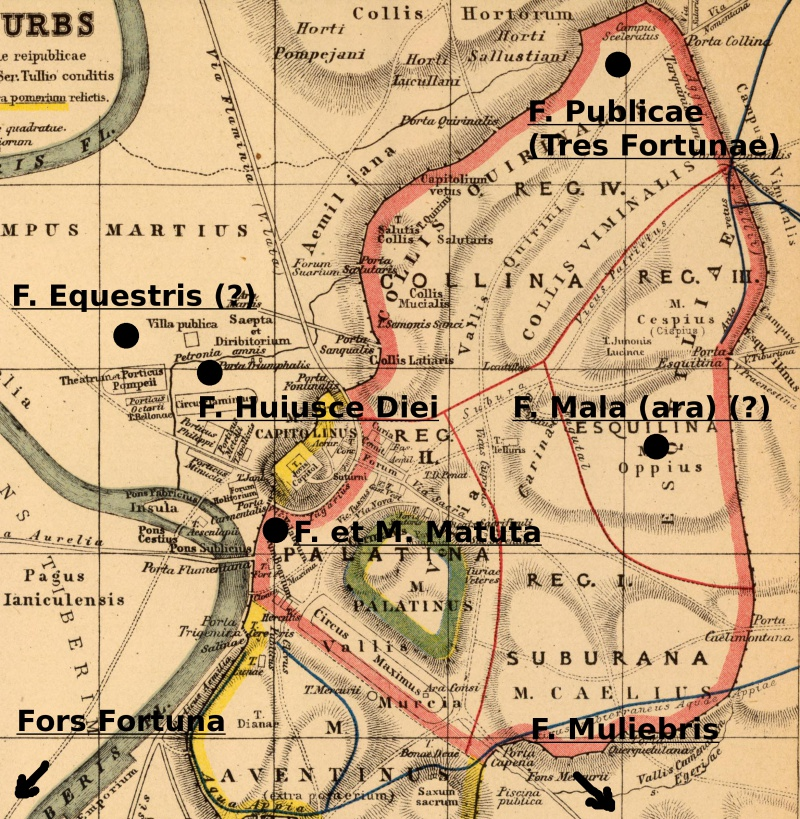
\includegraphics[scale=0.55]{images/roma_map1.jpg}}
\caption{Схема местоположения известных храмов Фортуны в Риме. \footnotesize{Источник оригинальной карты: \cite[Bl. XXII]{Kiepert1894}. }}
\label{pic:Charta}
\end{figure}


\chapter{Археологические свидетельства}

\section{Храм Фортуны на Бычьем форуме}\label{appendix:InForoBoario}

\begin{figure}[ht!]
\center{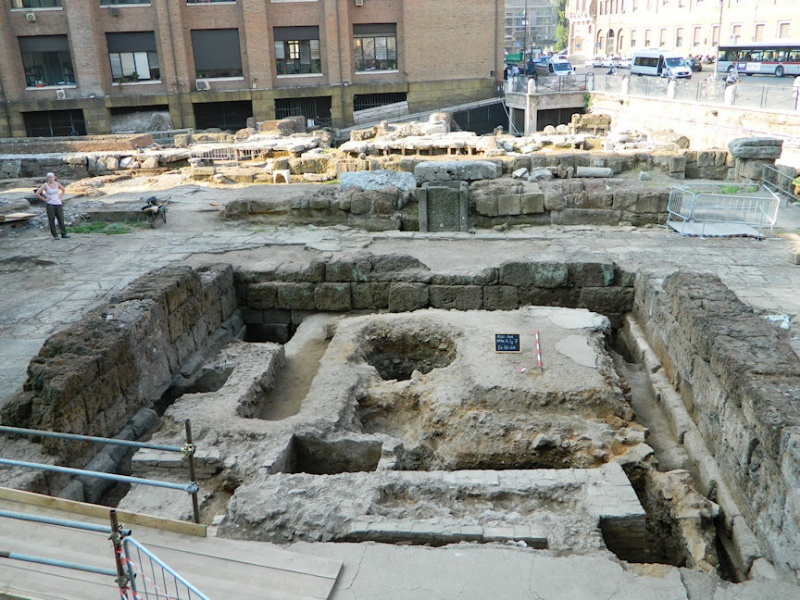
\includegraphics[scale=0.5]{images/figure1m.jpg}}
\caption{Общий вид раскопок в районе Сан-Омобоно. Современное состояние. \footnotesize{Источник: \cite[URL: \href{http://intarch.ac.uk/journal/issue31/1/images/figure1.html}{http://intarch.ac.uk/journal/issue31/1/images/figure1.html}]{Terrenato2012}}
}\label{pic:SOmobono1}
\end{figure}

\begin{figure}[ht!]
\center{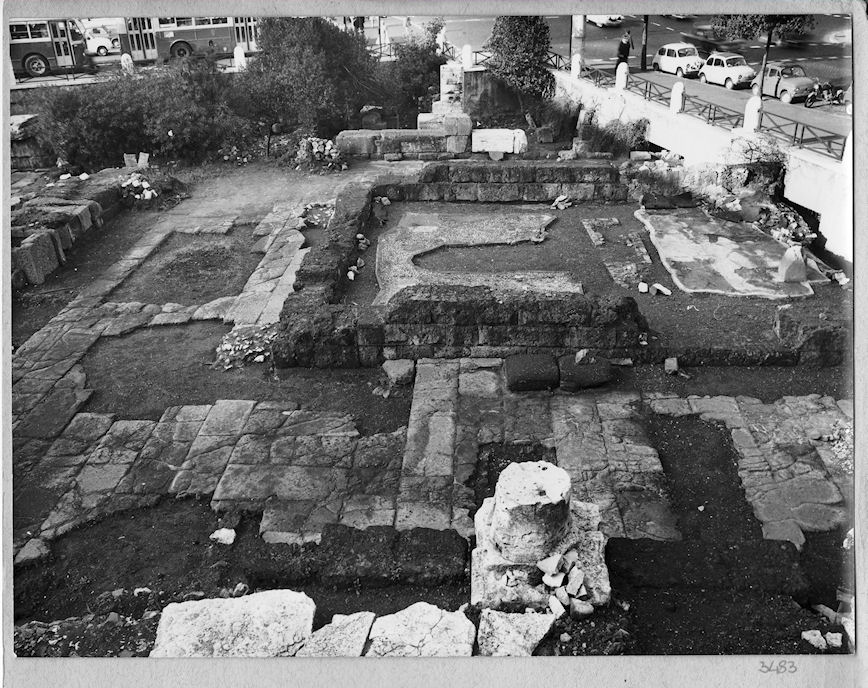
\includegraphics[scale=0.5]{images/figure62m.jpg}}
\caption{Вид на западный храм с запада (AFSRCM, S. Omobono, b. 29, 7, c. 3483).  \footnotesize{Источник: \cite[URL: \href{http://intarch.ac.uk/journal/issue31/1/images/figure62.html}{http://intarch.ac.uk/journal/issue31/1/images/figure62.html}]{Terrenato2012}}. }\label{pic:SOmobono2}
\end{figure}

%\pagebreak

\begin{figure}[ht!]
\center{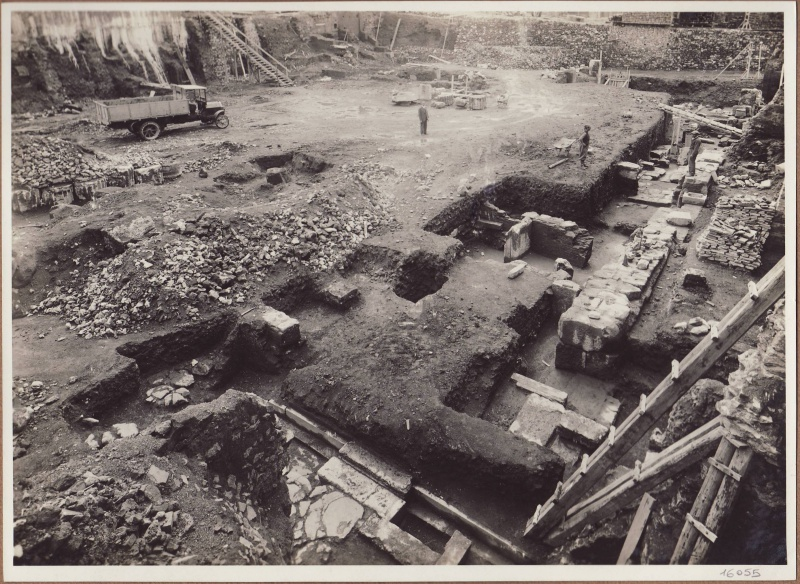
\includegraphics[scale=0.55]{images/figure32.jpg}}
\caption{Раскопки района церкви Сан-Омобоно в 1937 г.  \footnotesize{Источник: \cite[URL: \href{http://intarch.ac.uk/journal/issue31/1/images/figure32.html}{http://intarch.ac.uk/journal/issue31/1/images/figure32.html}]{Terrenato2012}}. }\label{pic:Excavatio1937}
\end{figure}

\begin{figure}[ht!]
\center{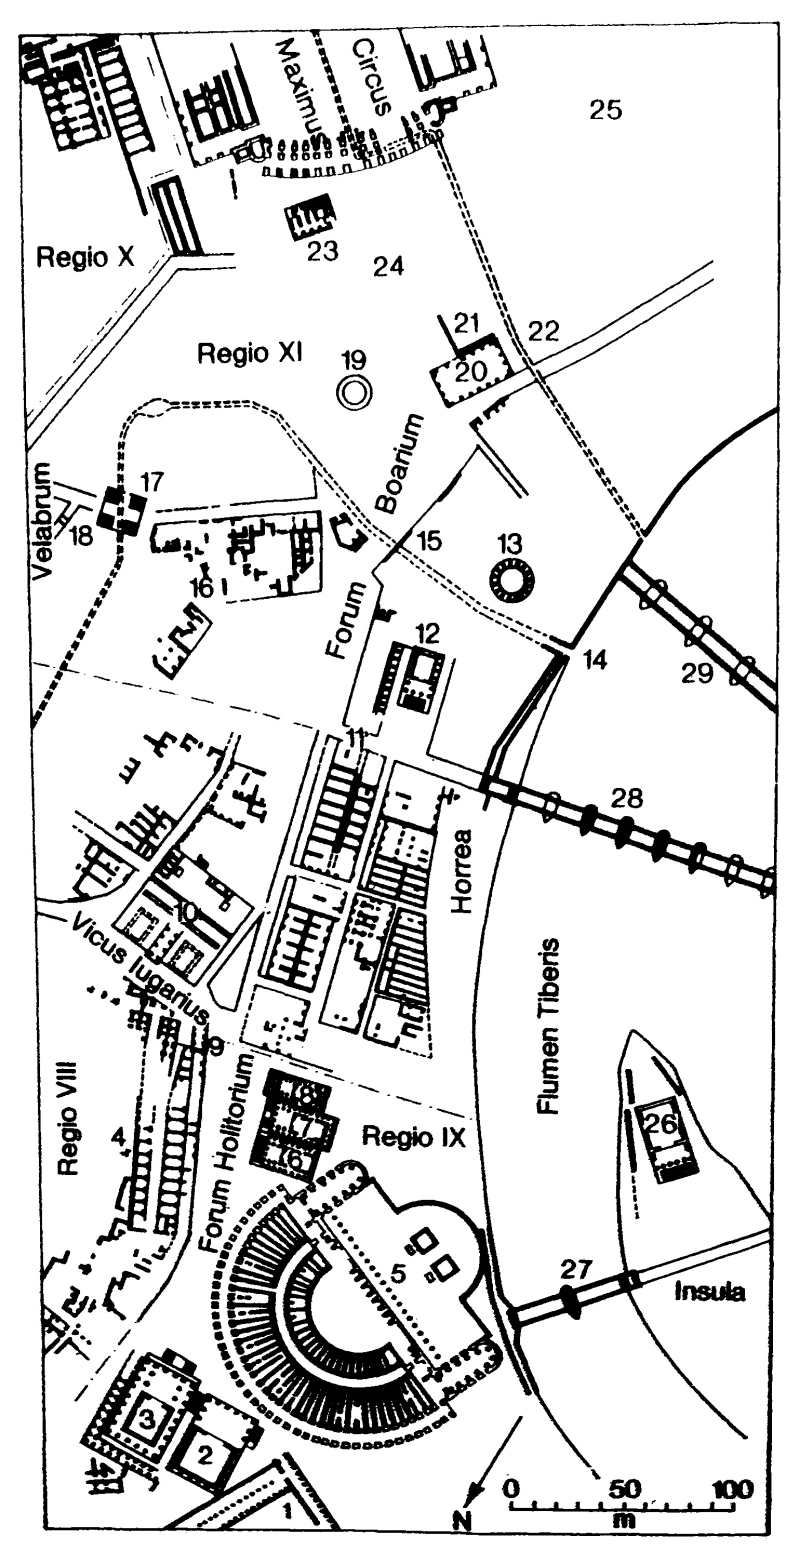
\includegraphics[scale=0.4]{images/fig02.jpg}}
\caption{Схема района Бычьего форума. Двойное святилище Фортуны и Матери Матуты обозначено под №~10. \footnotesize{Источник: \cite[P. 163]{Richardson1992}}. }
\label{pic:ForiBoariSchema}
\end{figure}

\begin{figure}[ht!]
\center{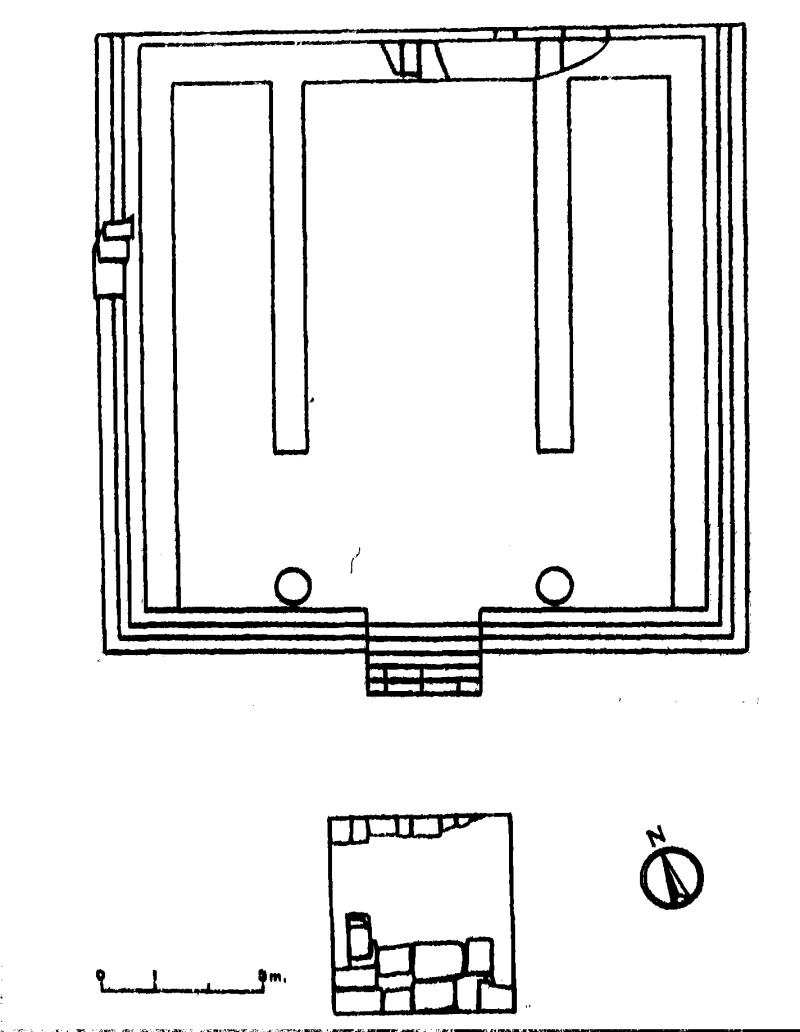
\includegraphics[scale=0.25]{images/fig04.jpg}}
\caption{Схема архаического храма в районе Сан-Омобоно (реконструкция). \footnotesize{Источник: \cite[P. 35]{Richardson1992}}. }\label{pic:ArchaicTemple1}
\end{figure}

\begin{figure}[ht!]
\center{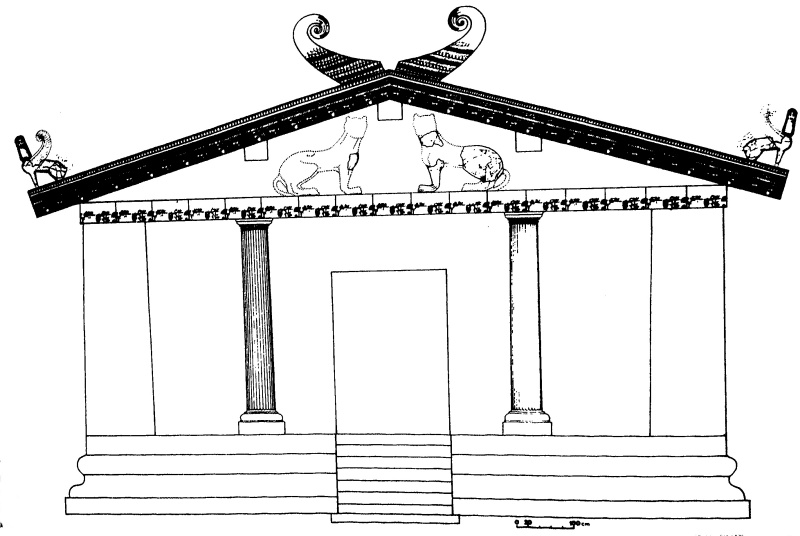
\includegraphics[scale=0.45]{images/fig05.jpg}}
\caption{Внешний вид архаического храма в районе Сан-Омобоно (реконструкция). \footnotesize{Источник: \cite[P. 36]{Richardson1992}}. }\label{pic:ArchaicTemple2}
\end{figure}

\begin{figure}[ht!]
\center{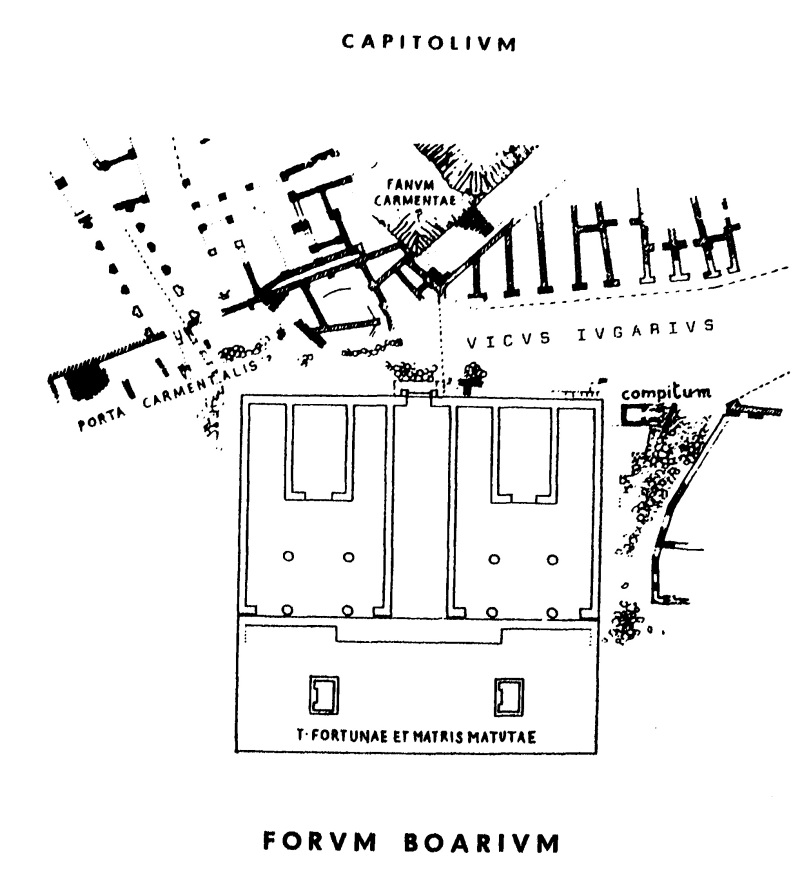
\includegraphics[scale=0.4]{images/fig03.jpg}}
\caption{Схема двойного храма Фортуны и Матери Матуты в районе Сан-Омобоно. Финальная фаза. \footnotesize{Источник: \cite[P. 35]{Richardson1992}}. }\label{pic:TwinTemples}
\end{figure}


\section{Aedes Fortunae Huiusce Diei}\label{appendix:FortunaHD}


\begin{figure}[ht!]
\center{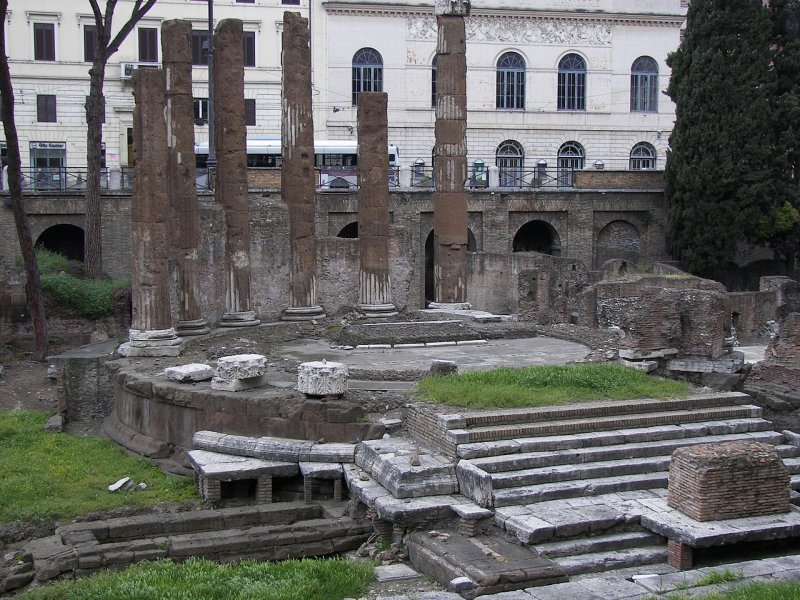
\includegraphics[scale=0.55]{images/forthd.jpg}}
\caption{Aedes Fortunae Huiusce Diei. Современное состояние. \footnotesize{}. }\label{pic:FortunaHD}
\end{figure}

\begin{figure}[ht!]
\center{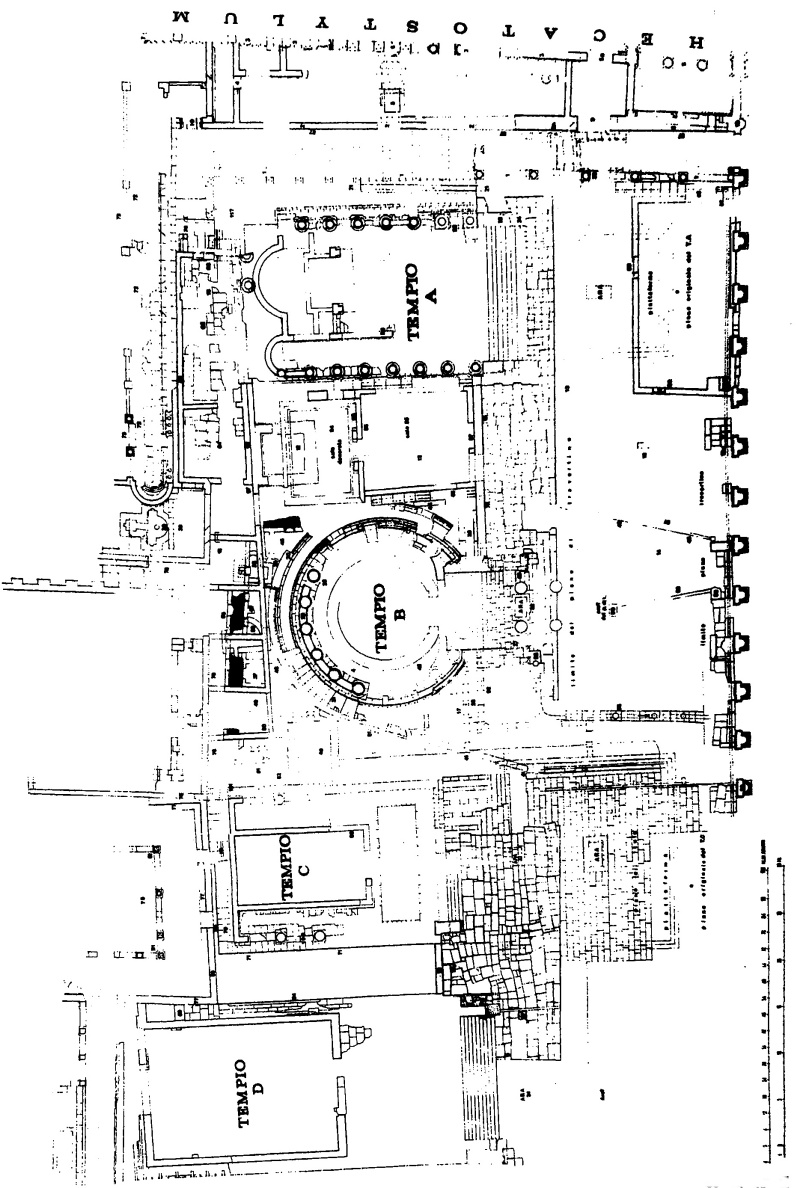
\includegraphics[scale=0.5]{images/forthd1.jpg}}
\caption{Общая схема Area Sacra di Largo Argentina. Храм Fortunae Huiusce Diei обозначен под литерой B. \footnotesize{Источник: \cite[P. 34]{Richardson1992}}. }
\end{figure}

\chapter{Монеты}

\begin{figure}[ht!]
\center{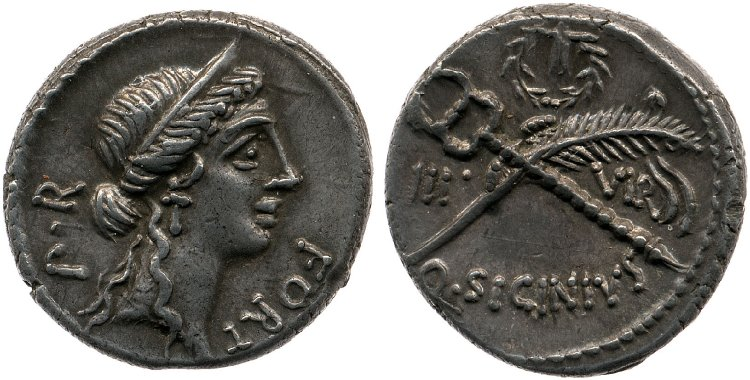
\includegraphics[scale=0.5]{images/RRC_440_1_1.jpg}}
\caption{Денарий с изображением Фортуны Римского Народа. Чеканка Рима, 49 г. до н.э. RRC 440/1. }\label{pic:RRC440}
\end{figure}

\begin{figure}[ht!]
\center{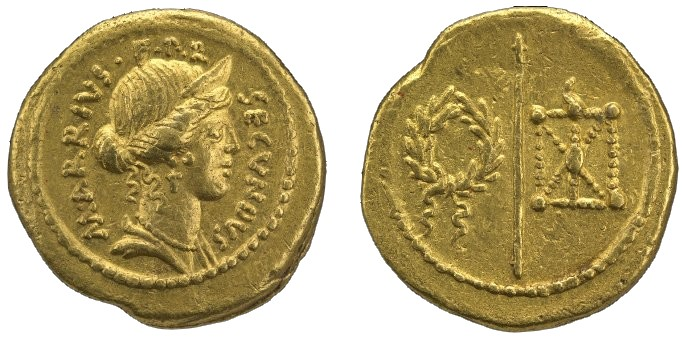
\includegraphics[scale=0.5]{images/RRC_513_1(1).jpg}}
\caption{Ауреус с изображением Фортуны Римского Народа. Чеканка Рима, 41 г. до н.э. RRC 513/1. }\label{pic:RRC513}
\end{figure}

\begin{figure}[ht!]
\center{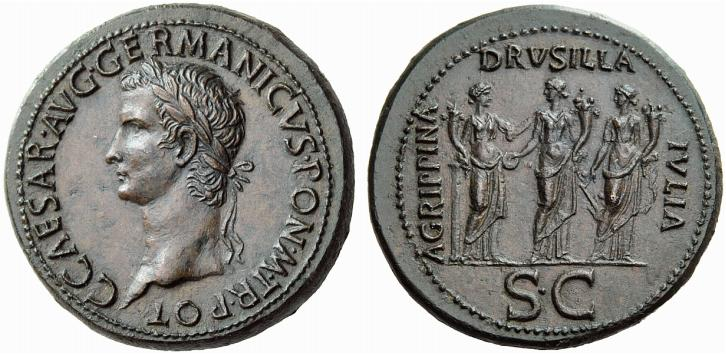
\includegraphics[scale=1.6]{images/ric_I_Caligula_33.jpg}}
\caption{Сестерций Калигулы с изображением трёх его сестёр. Агриппина изображена с атрибутами Секуритас, Друзилла "--- Конкордии, Юлия "--- Фортуны. Чеканка Рима, 37--38 гг. н.э. RIC I, Cal. 33.}\label{pic:CaligulaeSorores}
\end{figure}


\begin{figure}[ht!]
\center{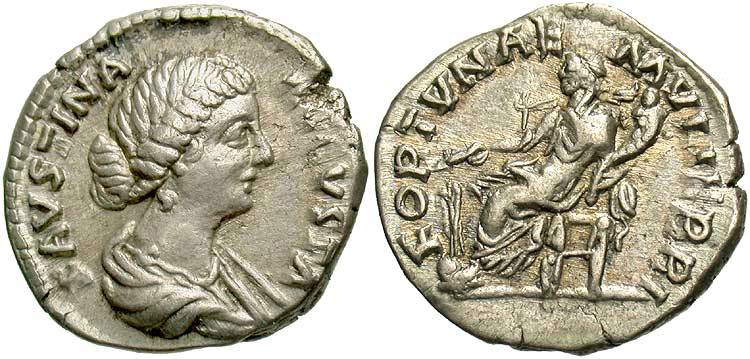
\includegraphics[scale=0.5]{images/RIC_III_Marcus_Aurelius_683.jpg}}
\caption{Денарий Марка Аврелия, посвящённый его жене, Фаустине Младшей, с изображением Женской Фортуны. RIC III, Marc. Aur. 683. }\label{pic:FortunaMuliebris}
\end{figure}

\chapter{Изображения Фортуны}\label{appendix:Pictura}

\begin{figure}[ht!]
\center{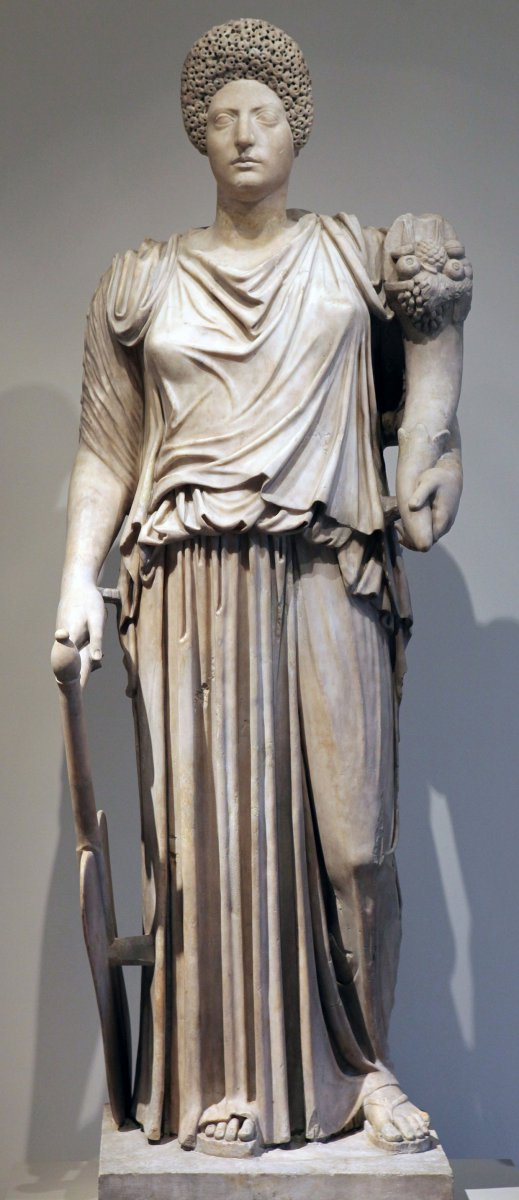
\includegraphics[scale=0.37]{images/sc0030.jpg}}
\caption{Статуя Тихи-Фортуны, мрамор, 2-я пол. I в. н.э. Нью-Йорк, музей Метрополитен. В результате реставрации кон. XVIII в. к статуе была приставлена голова неизвестной женщины (кон. I в. н.э.). \footnotesize{Фото и текст \textit{Роджер Б. Ульрих}. Источник: \href{http://ancientrome.ru/art/artwork/img.htm?id=4038}{http://ancientrome.ru/art/artwork/img.htm?id=4038}}}
\label{pic:FortunaFlav}
\end{figure}


\begin{figure}[ht!]
\center{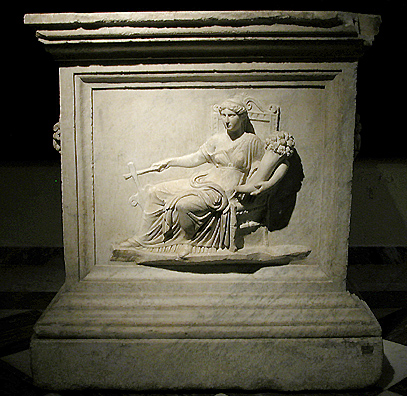
\includegraphics[scale=1.0]{images/ara_fortunae_1.jpg}}
\caption{Алтарь Фортуны, мрамор, датировка неизвестна. Рим, Капитолийский музей. \footnotesize{Фото \textit{Ann Raia}, 2007 г.}}
\label{pic:Ara1}
\end{figure}


\begin{figure}[ht!]
\center{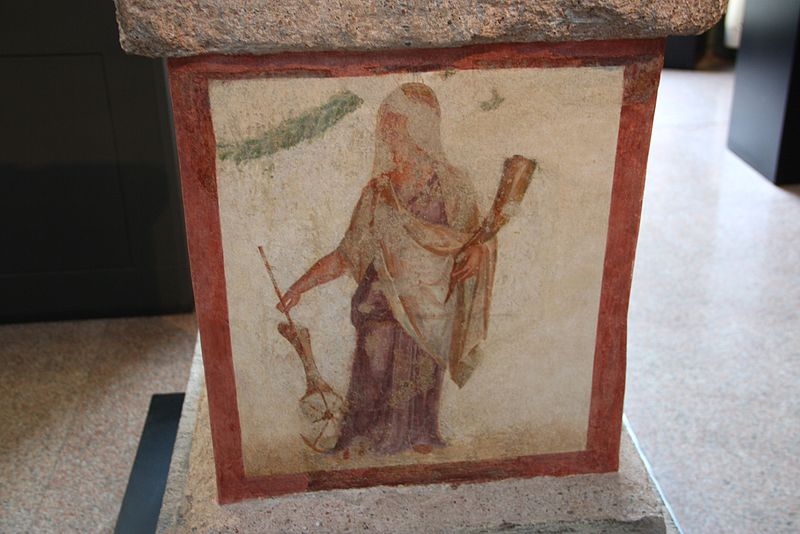
\includegraphics[scale=0.5]{images/ara_fortunae_2.jpg}}
\caption{Алтарь Фортуны, I--II вв. н.э. Миланский музей. \footnotesize{Фото \textit{Ann Raia}, 2007 г.}}
\label{pic:Ara2}
\end{figure}

\begin{figure}[ht!]
\center{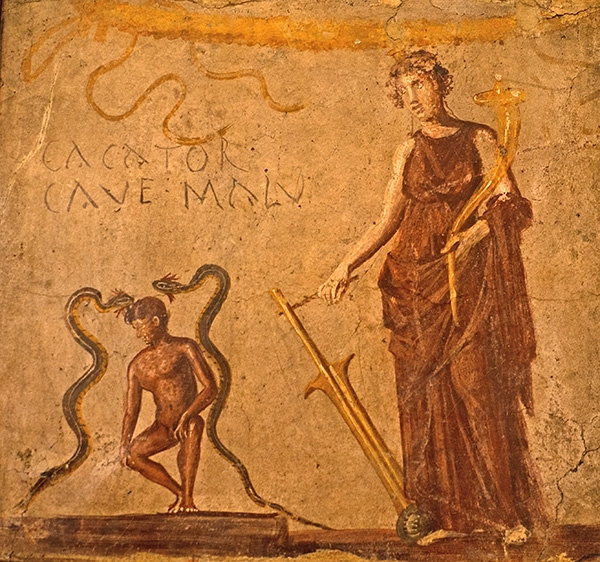
\includegraphics[scale=0.7]{images/cavemalum_fresco.jpg}}
\caption{Фреска с изображением Фортуны, Помпеи, I в. н.э. Неаполитанский музей. \footnotesize{Фото \textit{Barbara McManus}, 2012 г.}}
\label{pic:Cavemalum}
\end{figure}

\begin{figure}[ht!]
\center{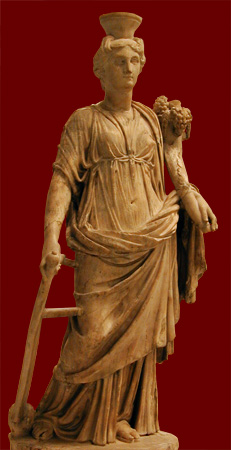
\includegraphics[scale=1.0]{images/fortuna_statue.jpg}}
\caption{Мраморная статуэтка Фортуны, 2-я пол. II в. н.э. Лондон, Британский музей. \footnotesize{Фото \textit{Barbara McManus}, 2001 г.}}
\label{pic:Fortuna2cent}
\end{figure}


\end{appendices}
 % Приложения

\end{document}

